



Topology is the study of spaces up to continuous deformation, and that is a slippery
thing to get a handle on. Given two spaces, how could we possibly hope to show that
there is \emph{no} homeomorphism between them? There are infinitely many candidate maps,
and no amount of failing to find one counts as a proof.

Algebraic topology answers this by translating the problem into algebra. We will build
machines that eat a topological space and spit out a group, in such a way that
homeomorphic (indeed, homotopy equivalent) spaces give isomorphic groups. Then two
spaces with non-isomorphic groups are certainly not homeomorphic, and a question with
infinitely many cases has become a finite computation. We will build two such machines:
the \emph{fundamental group}, which measures the failure of loops in a space to be
contracted to a point, and \emph{homology}, which detects holes of every dimension at
once. Along the way we will get some genuinely striking theorems almost for free --
that $\R^n \cong \R^m$ forces $n = m$, that every continuous map of a disc to itself has
a fixed point, and that every non-constant complex polynomial has a root.

This article constitutes my notes for the `Algebraic Topology' course, held in Michaelmas
2022 at Cambridge. These notes are \emph{not a transcription of the lectures}, and differ
significantly in quite a few areas. Still, all lectured material should be covered.



\section{The Fundamental Group}

Throughout these notes, a \vocab{space} means a topological space, and a \vocab{map}
means a continuous function -- we will say `function' when we do not want to assume
continuity. We write $X \cong Y$ to mean that $X$ and $Y$ are homeomorphic, and $G \cong H$
to mean that groups $G$ and $H$ are isomorphic. A few spaces will appear often enough to
deserve names:
\begin{itemize}
	\item the one-point space $*$;
	\item the unit interval $I = [0,1] \subseteq \R$, and the cube $I^n$;
	\item the disc $D^n = \{ v \in \R^n \mid \norm{v} \leq 1\}$, which is homeomorphic to $I^n$;
	\item the sphere $S^{n-1} = \{v \in \R^n \mid \norm{v} = 1\}$.
\end{itemize}
We write $\id_X$ for the identity map on $X$, and $c_p$ for a constant map with value $p$
(the domain being clear from context).

The two results we are aiming at in the first instance are that $\R^n \cong \R^m$ implies
$n = m$, and that every map $D^n \to D^n$ has a fixed point. For $n = 1$ both are easy:
removing a point from $\R$ disconnects it, which distinguishes $\R$ from $\R^m$ for
$m \geq 2$, and the fixed point statement is the intermediate value theorem. What we need
is a way of running these arguments in higher dimensions, and that requires something
finer than connectedness.

\subsection{Homotopy}

The right notion of `sameness' in this subject turns out not to be homeomorphism but
something coarser. We want to regard two maps as the same if one can be continuously
deformed into the other.

\begin{definition}[Homotopy]
	Let $f, g: X \rightarrow Y$ be maps. A \vocab{homotopy} from $f$ to $g$ is a map
	$$
	H: X \times I \rightarrow Y
	$$
	such that $H(x, 0)=f(x)$ and $H(x, 1)=g(x)$ for all $x \in X$.

	If such an $H$ exists, we say $f$ is \vocab{homotopic} to $g$, and write $f \simeq g$ or $f \simeq_H g$.
\end{definition}

We should think of the second coordinate as time: at each time $t \in I$ we have a map
$f_t = H(-, t): X \to Y$, and as $t$ runs from $0$ to $1$ these interpolate between $f$
and $g$. The content of continuity of $H$ is that the family $(f_t)$ varies continuously
in $t$, so there is no jumping.

\begin{center}
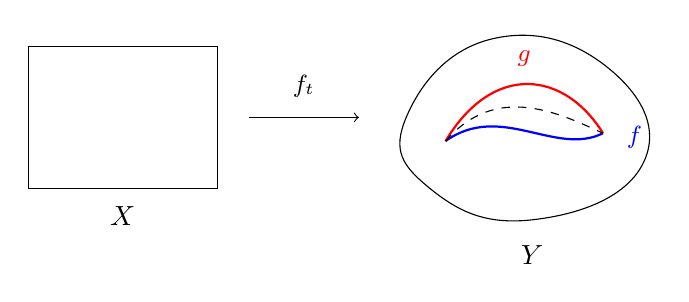
\begin{tikzpicture}[scale=1]
	% domain
	\draw[thin] (-0.2,-0.2) rectangle (2.2,1.6);
	\node at (1,-0.55) {$X$};
	% target blob
	\begin{scope}[xshift=4.6cm]
	\draw[thin] plot[smooth cycle, tension=0.8] coordinates {(0,0.7) (1.1,1.7) (2.6,1.3) (3.0,0.1) (1.6,-0.6) (0.3,-0.2)};
	\node at (1.6,-1.05) {$Y$};
	% images
	\draw[thick, color=blue] (0.5,0.4) .. controls (1.2,0.9) and (1.9,0.2) .. (2.5,0.5);
	\node[color=blue] at (2.9,0.45) {\small $f$};
	\draw[thick, color=red] (0.5,0.4) .. controls (1.1,1.4) and (2.0,1.3) .. (2.5,0.5);
	\node[color=red] at (1.5,1.45) {\small $g$};
	\draw[thin, dashed] (0.5,0.4) .. controls (1.15,1.15) and (1.95,0.75) .. (2.5,0.5);
	\end{scope}
	% arrow
	\draw[->] (2.6,0.7) -- (4.0,0.7);
	\node at (3.3,1.1) {\small $f_t$};
\end{tikzpicture}
\end{center}

Often we want to deform $f$ into $g$ without moving certain points at all.

\begin{definition}[Homotopy Relative to a Subspace]
	Let $A \subseteq X$. We say $f$ is homotopic to $g$ \vocab{relative to $A$}, written $f \simeq g \rel A$, if there is a homotopy $H$ from $f$ to $g$ with $H(a, t) = f(a) = g(a)$ for all $a \in A$ and all $t \in I$.
\end{definition}

Taking $A = \emptyset$ recovers ordinary homotopy, so it costs nothing to prove things in
this generality.

\begin{proposition}
	For spaces $X, Y$ and $A \subseteq X$, `homotopic $\rel A$' is an equivalence relation on maps $X \to Y$. In particular, when $A = \emptyset$, homotopy is an equivalence relation.
\end{proposition}
\begin{proof}
	We check the three properties.
	\begin{enumerate}
		\item \emph{Reflexivity}: $f \simeq f$ since $H(x, t)=f(x)$ is a homotopy.
		\item \emph{Symmetry}: if $H(x, t)$ is a homotopy from $f$ to $g$, then $H(x, 1-t)$ is a homotopy from $g$ to $f$.
		\item \emph{Transitivity}: Suppose $f, g, h: X \rightarrow Y$ and $f \simeq_H g \rel A$, $g \simeq_{H^{\prime}} h \rel A$. We want to show that $f \simeq h \rel A$. The idea is to `glue' the two homotopies together: we know how to continuously deform $f$ to $g$, and $g$ to $h$, so we just do these one after another, at double speed. We define $H^{\prime \prime}: X \times I \rightarrow Y$ by
		$$
		H^{\prime \prime}(x, t)= \begin{cases}H(x, 2 t) & 0 \leq t \leq \frac{1}{2} \\ H^{\prime}(x, 2 t-1) & \frac{1}{2} \leq t \leq 1.\end{cases}
		$$
		This is well-defined since $H(x, 1)=g(x)=H^{\prime}(x, 0)$, and continuous by the gluing lemma. It is easy to check that $H''$ is a homotopy $\rel A$. \qedhere
	\end{enumerate}
\end{proof}

We used the gluing lemma there, and we will use it constantly, so let us record it.

\begin{lemma}[Gluing Lemma]
	Let $X = C_1 \cup C_2$ with $C_1, C_2$ closed in $X$, and let $f: X \to Y$ be a function such that $f|_{C_1}$ and $f|_{C_2}$ are both continuous. Then $f$ is continuous.
\end{lemma}
\begin{proof}
	It is enough to show that preimages of closed sets are closed. Let $K \subseteq Y$ be closed. Then $f^{-1}(K) \cap C_i = (f|_{C_i})^{-1}(K)$ is closed in $C_i$, and hence closed in $X$ as $C_i$ is closed in $X$. So $f^{-1}(K) = (f^{-1}(K) \cap C_1) \cup (f^{-1}(K) \cap C_2)$ is a union of two closed sets, and is closed.
\end{proof}

Homotopy behaves well under composition, which is what makes the whole theory work.

\begin{lemma} \label{lem:homotopy-composition}
	Consider the spaces and maps
	% https://q.uiver.app/#q=WzAsMyxbMCwwLCJYIl0sWzEsMCwiWSJdLFsyLDAsIloiXV0=
	\[\begin{tikzcd}
		X & Y & Z
		\arrow["{f_0}", curve={height=-12pt}, from=1-1, to=1-2]
		\arrow["{g_0}", curve={height=-12pt}, from=1-2, to=1-3]
		\arrow["{f_1}"', curve={height=12pt}, from=1-1, to=1-2]
		\arrow["{g_1}"', curve={height=12pt}, from=1-2, to=1-3]
	\end{tikzcd}\]
	If $f_0 \simeq_H f_1$ and $g_0 \simeq_{H'} g_1$, then $g_0 \circ f_0 \simeq g_1 \circ f_1$.
\end{lemma}
\begin{proof}
	We will show that $g_0 \circ f_0 \simeq g_0 \circ f_1 \simeq g_1 \circ f_1$, and will then be done since homotopy is an equivalence relation. We write down two homotopies.
	\begin{enumerate}
		\item The composition
		\[\begin{tikzcd}
			{X\times I} & Y & Z
			\arrow["H", from=1-1, to=1-2]
			\arrow["{g_0}", from=1-2, to=1-3]
		\end{tikzcd}\]
		is the first homotopy we need, showing $g_0 \circ f_0 \simeq g_0 \circ f_1$.
		\item The following composition is a homotopy from $g_0 \circ f_1$ to $g_1 \circ f_1$:
		\[\begin{tikzcd}
			{X\times I} & {Y\times I} & Z
			\arrow["{f_1 \times \id_I}", from=1-1, to=1-2]
			\arrow["{H'}", from=1-2, to=1-3]
		\end{tikzcd}\]
		Indeed at $t=0$ this is $H'(f_1(x), 0) = g_0(f_1(x))$ and at $t = 1$ it is $g_1(f_1(x))$. \qedhere
	\end{enumerate}
\end{proof}

Now that we have a notion of two maps being `the same', we get a notion of two spaces
being the same: we ask for maps in both directions whose composites are homotopic to,
rather than equal to, the identity.

\begin{definition}[Homotopy Equivalence]
	A map $f: X \rightarrow Y$ is a \vocab{homotopy equivalence} if there exists a map $g:Y \rightarrow X$ such that $f \circ g \simeq \id_Y$ and $g \circ f \simeq \id_X$. We call $g$ a \vocab{homotopy inverse} for $f$.

	If a homotopy equivalence $f: X \rightarrow Y$ exists, we say $X$ and $Y$ are \vocab{homotopy equivalent}, and write $X \simeq Y$.
\end{definition}

Note the deliberate abuse: $\simeq$ means homotopy for maps and homotopy equivalence for
spaces. Any homeomorphism is in particular a homotopy equivalence, so $X \cong Y$ implies
$X \simeq Y$, but the converse fails badly -- as we will see, $\R^2$ is homotopy
equivalent to a point.

\begin{proposition}
	Homotopy equivalence of spaces is an equivalence relation.
\end{proposition}
\begin{proof}
	Symmetry and reflexivity are immediate from the definition. To show transitivity, let $f:X \rightarrow Y$ and $h: Y \rightarrow Z$ be homotopy equivalences, and $g: Y \rightarrow X$ and $k: Z \rightarrow Y$ be their homotopy inverses. We will show that $h \circ f : X \rightarrow Z$ is a homotopy equivalence with homotopy inverse $g \circ k$. Using Lemma \ref{lem:homotopy-composition} freely, we have
	\begin{align*}
		(h \circ f) \circ (g \circ k) = h \circ (f \circ g) \circ k \simeq h \circ \id_Y \circ\, k = h \circ k \simeq \id_Z.
	\end{align*}
	Similarly,
	\begin{align*}
		(g \circ k) \circ(h \circ f)=g \circ(k \circ h) \circ f \simeq g \circ \id_Y \circ\, f=g \circ f \simeq \id_X,
	\end{align*}
	as required.
\end{proof}

\begin{definition}[Contractible]
	If $X \simeq *$, the one point space, then $X$ is \vocab{contractible}.
\end{definition}

Unwinding this, $X$ is contractible exactly when $\id_X \simeq c_p$ for some $p \in X$;
the homotopy is a way of continuously shrinking the whole space down to a point inside
itself.

\begin{example}
	Any non-empty convex $Y \subseteq \R^n$ is contractible. Indeed, fix $p \in Y$ and define $H(y, t) = (1-t)y + tp$, which lies in $Y$ by convexity and is a homotopy from $\id_Y$ to $c_p$. In particular $\R^n$ and $D^n$ and $I^n$ are all contractible.
\end{example}

\begin{proposition} \label{prop:contractible-maps}
	Let $Y$ be contractible. Then any two maps $f_0, f_1: X \to Y$ are homotopic.
\end{proposition}
\begin{proof}
	Say $\id_Y \simeq c_p$. Then $f_0 = \id_Y \circ f_0 \simeq c_p \circ f_0 = c_p$, and likewise $f_1 \simeq c_p$, so $f_0 \simeq f_1$ by transitivity.
\end{proof}

\begin{corollary}
	A contractible space is path connected.
\end{corollary}
\begin{proof}
	Let $p, q \in Y$. Applying Proposition \ref{prop:contractible-maps} with $X = *$, the constant maps $* \to Y$ at $p$ and at $q$ are homotopic via some $H: * \times I \to Y$. Then $t \mapsto H(*, t)$ is a path from $p$ to $q$.
\end{proof}

A very common way of exhibiting a homotopy equivalence is to squash a space down onto a
subspace sitting inside it.

\begin{definition}[Retraction]
	Let $A \subseteq X$ be a subspace. A \vocab{retraction} $r:X \rightarrow A$ is a map such that $r \circ \iota = \id_A$, where $\iota: A \hookrightarrow X$ is the inclusion. If such an $r$ exists, we call $A$ a \vocab{retract} of $X$.

	The retraction $r$ is a \vocab{deformation retraction} if $\iota \circ r \simeq \id_X$. A deformation retraction is \vocab{strong} if we require this homotopy to be a homotopy $\rel A$.
\end{definition}

If $r: X \to A$ is a deformation retraction then $r$ is by definition a homotopy
equivalence, with homotopy inverse $\iota$. So $A \simeq X$.

\begin{example} \label{ex:sdr-sphere}
	The map $r: \R^{n+1} \setminus \{0\} \to S^n$ given by $r(v) = v/\norm{v}$ is a strong deformation retraction. Indeed $r \circ \iota = \id_{S^n}$, and
	$$
	H(v, t) = \frac{v}{(1-t) + t\norm{v}}
	$$
	is a homotopy from $\id$ to $\iota \circ r$ fixing $S^n$ pointwise. So $\R^{n+1} \setminus \{0\} \simeq S^n$: the punctured space is homotopy equivalent to the sphere, even though the two are very far from homeomorphic.
\end{example}

\begin{center}
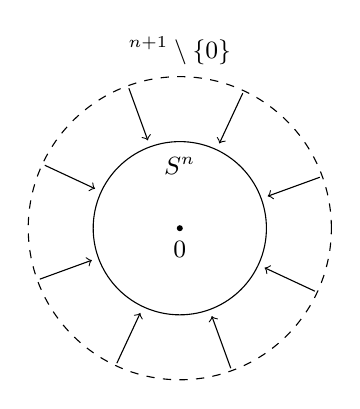
\begin{tikzpicture}[scale=1.1]
	\draw[thin] (0,0) circle (1);
	\draw[thin, dashed] (0,0) circle (1.75);
	\foreach \a in {20,65,110,155,200,245,290,335} {
		\draw[->, thin] (\a:1.72) -- (\a:1.08);
	}
	\fill (0,0) circle (0.035);
	\node at (0,-0.25) {\small $0$};
	\node at (0,0.72) {\small $S^n$};
	\node at (0,2.05) {\small $\R^{n+1}\setminus\{0\}$};
\end{tikzpicture}
\end{center}

\subsection{Paths}

We now specialise to the maps that will give us our invariant. The idea is very simple:
we probe a space $X$ by mapping intervals into it, and see which of the resulting loops
can be contracted.

\begin{definition}[Path]
	A \vocab{path} in a space $X$ is a map $\gamma: I \rightarrow X$.
	If $\gamma(0) = x_0$ and $\gamma(1) = x_1$, we say $\gamma$ is a path from $x_0$ to $x_1$, and write $\gamma: x_0 \leadsto x_1$.

	If $\gamma(0) = \gamma(1) = x_0$, we say $\gamma$ is a \vocab{loop} (based at $x_0$).
\end{definition}

We write $\Omega(X, x_0, x_1)$ for the set of paths $x_0 \leadsto x_1$ in $X$, and
$\Omega(X, x_0) = \Omega(X, x_0, x_0)$ for the set of loops based at $x_0$.

\begin{definition}[Concatenation and Inverses]
	If we have two paths $\gamma_1$ from $x_0$ to $x_1$ and $\gamma_2$ from $x_1$ to $x_2$, we define the \vocab{concatenation} to be
	$$
	(\gamma_1 \cdot \gamma_2)(t) = \begin{cases}
		\gamma_1(2t) & 0 \leq t \leq \frac{1}{2}\\
		\gamma_2(2t - 1) & \frac{1}{2} \leq t \leq 1.
	\end{cases}
	$$
	This is continuous by the gluing lemma.

	The \vocab{inverse} of a path $\gamma: I \rightarrow X$ is defined by
	$$
	\gamma^{-1}(t) = \gamma(1 -t).
	$$

	The \vocab{constant path} at a point $x \in X$ is given by $c_x(t) = x$.
\end{definition}

So $\gamma_1 \cdot \gamma_2$ traverses $\gamma_1$ at double speed, then $\gamma_2$ at
double speed, and $\gamma^{-1}$ runs $\gamma$ backwards.

\begin{center}
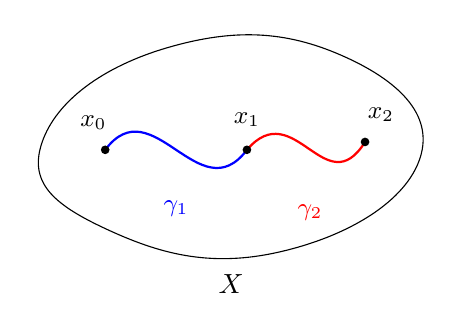
\begin{tikzpicture}[scale=1]
	\draw[thin] plot[smooth cycle, tension=0.8] coordinates {(-0.4,0.4) (1.2,1.6) (3.4,1.5) (4.4,0.2) (2.6,-1.0) (0.4,-0.7)};
	\node at (2.0,-1.4) {$X$};
	\draw[thick, color=blue] (0.4,0.3) .. controls (1.0,1.1) and (1.6,-0.5) .. (2.2,0.3);
	\draw[thick, color=red] (2.2,0.3) .. controls (2.8,1.0) and (3.2,-0.4) .. (3.7,0.4);
	\fill (0.4,0.3) circle (0.055); \node at (0.25,0.65) {\small $x_0$};
	\fill (2.2,0.3) circle (0.055); \node at (2.2,0.68) {\small $x_1$};
	\fill (3.7,0.4) circle (0.055); \node at (3.9,0.75) {\small $x_2$};
	\node[color=blue] at (1.3,-0.45) {\small $\gamma_1$};
	\node[color=red] at (3.0,-0.5) {\small $\gamma_2$};
\end{tikzpicture}
\end{center}

We would like to make $\Omega(X, x_0)$ into a group under concatenation, and the reader
will immediately object that this cannot work: concatenation is not associative on the
nose, since $(\gamma_0 \cdot \gamma_1) \cdot \gamma_2$ and
$\gamma_0 \cdot (\gamma_1 \cdot \gamma_2)$ traverse the three paths at different speeds.
The fix is to pass to homotopy classes, and here we must be careful to only allow
homotopies which fix the endpoints -- otherwise every loop could be slid off to a
constant and nothing would be left.

\begin{definition}[Homotopy of Paths]
	Paths $\gamma, \gamma': I \rightarrow X$ are \vocab{homotopic as paths} if they are homotopic $\rel \{0, 1\} \subseteq I$, that is, if the endpoints stay fixed throughout. We write $\gamma \simeq \gamma'$.
\end{definition}

Concretely, $\gamma \simeq \gamma'$ means there is a map $H: I \times I \to X$ with
$H(s, 0) = \gamma(s)$, $H(s,1) = \gamma'(s)$, and $H(0,t) = x_0$, $H(1,t) = x_1$ for all
$t$. It is worth drawing the square: the bottom edge is $\gamma$, the top edge is
$\gamma'$, and the two vertical edges are constant.

\begin{center}
\begin{tikzpicture}[scale=1.5]
	\draw[thin] (0,0) rectangle (2,1.4);
	\draw[thick, color=blue] (0,0) -- (2,0);
	\draw[thick, color=red] (0,1.4) -- (2,1.4);
	\node[color=blue, below] at (1,-0.03) {\small $\gamma$};
	\node[color=red, above] at (1,1.43) {\small $\gamma'$};
	\node[left] at (-0.05,0.7) {\small $c_{x_0}$};
	\node[right] at (2.05,0.7) {\small $c_{x_1}$};
	\node at (1,0.7) {\small $H$};
	\fill (0,0) circle (0.03); \fill (2,0) circle (0.03);
	\fill (0,1.4) circle (0.03); \fill (2,1.4) circle (0.03);
	\draw[->] (2.65,0.7) -- (3.25,0.7);
	\begin{scope}[xshift=3.6cm, yshift=-0.1cm]
		\draw[thin] plot[smooth cycle, tension=0.85] coordinates {(0,0.7) (1.0,1.7) (2.4,1.4) (2.7,0.2) (1.4,-0.6) (0.2,-0.1)};
		\draw[thick, color=blue] (0.45,0.4) .. controls (1.0,-0.15) and (1.7,0.1) .. (2.2,0.55);
		\draw[thick, color=red] (0.45,0.4) .. controls (1.0,1.3) and (1.7,1.1) .. (2.2,0.55);
		\draw[thin, dashed] (0.45,0.4) .. controls (1.0,0.55) and (1.7,0.6) .. (2.2,0.55);
		\fill (0.45,0.4) circle (0.045); \fill (2.2,0.55) circle (0.045);
		\node at (1.35,-1.0) {$X$};
	\end{scope}
\end{tikzpicture}
\end{center}

\begin{lemma}[The Group Operation is Well-Defined] \label{lem:concat-well-defined}
	Let $\gamma_1, \gamma_2: I \rightarrow X$ be paths with $\gamma_1(1) = \gamma_2(0)$. Then if $\gamma_1 \simeq \gamma_1'$ and $\gamma_2 \simeq \gamma_2'$, we have $\gamma_1 \cdot \gamma_2 \simeq \gamma_1' \cdot \gamma_2'$.
\end{lemma}
\begin{proof}
	Suppose that $\gamma_1 \simeq_{H_1} \gamma_1'$ and $\gamma_2 \simeq_{H_2} \gamma_2'$. Then we can construct the homotopy
	$$
	H(s, t)= \begin{cases}H_1(2 s, t) & 0 \leq s \leq \frac{1}{2} \\ H_2(2 s-1, t) & \frac{1}{2} \leq s \leq 1,\end{cases}
	$$
	which is well-defined since $H_1(1,t) = \gamma_1(1) = \gamma_2(0) = H_2(0,t)$, and continuous by the gluing lemma. It visibly fixes the endpoints.
\end{proof}

\begin{lemma}[Indeed a Group Operation] \label{lem:group-op}
	Let $\gamma_0: x_0 \leadsto x_1$, $\gamma_1: x_1 \leadsto x_2$, $\gamma_2: x_2 \leadsto x_3$ be paths.
	Then
	\begin{enumerate}
		\item $(\gamma_0 \cdot \gamma_1) \cdot \gamma_2 \simeq \gamma_0 \cdot (\gamma_1 \cdot \gamma_2)$.
		\item $\gamma_0 \cdot c_{x_1} \simeq \gamma_0 \simeq c_{x_0} \cdot \gamma_0$.
		\item $\gamma_0 \cdot \gamma_0^{-1} \simeq c_{x_0}$ and $\gamma_0^{-1} \cdot \gamma_0 \simeq c_{x_1}$.
	\end{enumerate}
\end{lemma}
\begin{proof}
	We first note that the composition of any path $\gamma$ with an order-preserving surjection $\phi: I \rightarrow I$ is homotopic as paths to the original path, via $H(s, t) = \gamma(t\phi(s) + (1 - t)s)$. Such a $\phi$ is called a \vocab{reparameterisation}, and the homotopy fixes endpoints because $\phi(0) = 0$ and $\phi(1) = 1$.
	\begin{enumerate}
		\item Take $\phi$ to be the function
		$$
		\phi(t)=\begin{cases}
			\frac{t}{2} & 0 \leq t \leq \frac{1}{2} \\
			t - \frac{1}{4} & \frac{1}{2} \leq t \leq \frac{3}{4} \\
			2t - 1 & \frac{3}{4} \leq t \leq 1.
		\end{cases}
		$$
		Then we have $(\gamma_0 \cdot \gamma_1) \cdot \gamma_2 \simeq ((\gamma_0 \cdot \gamma_1) \cdot \gamma_2) \circ \phi = \gamma_0 \cdot (\gamma_1 \cdot \gamma_2)$.
		\item To see $\gamma_0 \cdot c_{x_1} \simeq \gamma_0$, reparameterise $\gamma_0$ with
		$$
		t \mapsto \begin{cases}
			2t & 0 \leq t \leq \frac{1}{2} \\
			1 & \frac{1}{2} \leq t \leq 1,
		\end{cases}
		$$
		and the other side is analogous.
		\item We have that $c_{x_0} \simeq \gamma_0 \cdot \gamma_0^{-1}$ via
		$$
		H(s, t) = \begin{cases}
			\gamma_0(2s) & 0 \leq s \leq \frac{t}{2} \\
			\gamma_0(t) & \frac{t}{2} \leq s \leq 1 - \frac{t}{2} \\
			\gamma_0^{-1}(2s - 1) & 1 - \frac{t}{2} \leq s \leq 1.
		\end{cases}
		$$
		At time $t$ this path runs along $\gamma_0$ as far as $\gamma_0(t)$, waits there, and comes back; at $t = 0$ it is constant and at $t=1$ it is $\gamma_0 \cdot \gamma_0^{-1}$. Applying this to $\gamma_0^{-1}$ gives the other identity. \qedhere
	\end{enumerate}
\end{proof}

\subsection{The Fundamental Group}

We can now define one of our central objects of study.

\begin{definition}[Fundamental Group]
	Let $X$ be a space and $x_0 \in X$. The \vocab{fundamental group} of $X$ (based at $x_0$), denoted $\pi_1(X, x_0)$, is the set of homotopy classes of loops in $X$ based at $x_0$, that is, $\pi_1(X, x_0) = \Omega(X, x_0)/\simeq$.

	The group operation is defined by $[\gamma_0][\gamma_1] = [\gamma_0 \cdot \gamma_1]$, with $[\gamma]^{-1} = [\gamma^{-1}]$ and identity the class $e = [c_{x_0}]$ of the constant path.
\end{definition}

\begin{theorem}
	The fundamental group is a group.
\end{theorem}
\begin{proof}
	The operation is well-defined by Lemma \ref{lem:concat-well-defined}, and the group axioms hold by Lemma \ref{lem:group-op}.
\end{proof}

The definition depends on a choice of basepoint, and we will deal with that dependence
shortly. First, let us see that $\pi_1$ is not just an invariant of spaces, but of maps
as well -- this is what makes it useful.

\begin{definition}[Based Space]
	A \vocab{based space} is a pair $(X, x_0)$ of a space $X$ and a point $x_0 \in X$, the \vocab{basepoint}. A \vocab{map of based spaces} $f: (X, x_0) \rightarrow (Y, y_0)$ is a map $f: X \rightarrow Y$ such that $f(x_0) = y_0$. A \vocab{based homotopy} is a homotopy $\rel \{x_0\}$.
\end{definition}

\begin{proposition}[$\pi_1$ is a Functor] \label{prop:functor}
	To a based map $f: (X, x_0) \rightarrow (Y, y_0)$, there is an associated function
	$f_* = \pi_1(f): \pi_1(X, x_0) \rightarrow \pi_1(Y, y_0)$, defined by $[\gamma] \mapsto [f \circ \gamma]$. Moreover it satisfies
	\begin{enumerate}
		\item $\pi_1(f)$ is a homomorphism of groups.
		\item If $f \simeq f' \rel \{x_0\}$, then $\pi_1(f) = \pi_1(f')$.
		\item For any based maps $(A, a) \stackrel{h}{\longrightarrow}(B, b) \stackrel{k}{\longrightarrow}(C, c)$, we have $\pi_1(k \circ h)= \pi_1(k) \circ \pi_1(h)$.
		\item $\pi_1(\id_X) = \id_{\pi_1(X, x_0)}$.
	\end{enumerate}
\end{proposition}
\begin{proof}
	First, $f_*$ is well-defined: if $\gamma \simeq_H \gamma'$ as paths, then $f \circ H$ is a homotopy of paths from $f \circ \gamma$ to $f \circ \gamma'$.

	For (i), observe that composing with $f$ commutes with concatenation,
	$$
	(f \circ (\gamma \cdot \gamma'))(t) = \begin{cases} f(\gamma(2t)) & t \leq \tfrac12 \\ f(\gamma'(2t-1)) & t \geq \tfrac12\end{cases} = ((f\circ\gamma)\cdot(f\circ\gamma'))(t),
	$$
	so $f_*([\gamma][\gamma']) = [f \circ (\gamma\cdot\gamma')] = [f\circ\gamma][f\circ\gamma'] = f_*[\gamma] f_*[\gamma']$.

	For (ii), if $H$ is a based homotopy from $f$ to $f'$ and $\gamma$ is a loop at $x_0$, then $(s,t) \mapsto H(\gamma(s), t)$ is a homotopy of paths from $f \circ \gamma$ to $f' \circ \gamma$: it fixes the endpoints since $\gamma(0) = \gamma(1) = x_0$ and $H(x_0, t) = y_0$ for all $t$.

	Parts (iii) and (iv) are immediate: $(k \circ h)_*[\gamma] = [k \circ h \circ \gamma] = k_*[h \circ \gamma] = k_*h_*[\gamma]$, and $(\id_X)_*[\gamma] = [\gamma]$.
\end{proof}

In the language of categories, $\pi_1$ is a functor from based spaces to groups. The
following diagram, expressing part (iii), commutes.
\[\begin{tikzcd}
	{\pi_1(X,x_0)} \arrow[rr, "{(g \circ f)_*}"] \arrow[rd, "f_*"'] & & {\pi_1(Z,z_0)} \\
	& {\pi_1(Y,y_0)} \arrow[ru, "g_*"'] &
\end{tikzcd}\]

This gives us our first real payoff, essentially for free.

\begin{corollary} \label{cor:homeo-iso}
	If $f: X \to Y$ is a homeomorphism with $f(x_0) = y_0$, then $f_*: \pi_1(X,x_0) \to \pi_1(Y,y_0)$ is an isomorphism.
\end{corollary}
\begin{proof}
	Apply the functor to $f \circ f^{-1} = \id_Y$ and $f^{-1} \circ f = \id_X$ to get $f_* \circ (f^{-1})_* = \id$ and $(f^{-1})_* \circ f_* = \id$.
\end{proof}

\subsection{Change of Basepoint}

We want to remove the basepoint dependence of the fundamental group. Of course we cannot
hope to compare $\pi_1(X, x_0)$ and $\pi_1(X, x_1)$ when $x_0$ and $x_1$ lie in different
path components, since a loop at $x_0$ knows nothing about the rest of $X$. But if there
is a path between them we can drag loops along it.

\begin{proposition} \label{prop:change-basepoint}
	A path $u: x_0 \leadsto x_1$ induces a group isomorphism $u_\#: \pi_1(X, x_0) \rightarrow \pi_1(X, x_1)$ by $[\gamma] \mapsto [u^{-1} \cdot \gamma \cdot u]$. This satisfies
	\begin{enumerate}
		\item If $u \simeq u'$, then $u_\# = u'_\#$.
		\item $(c_{x_0})_\# = \id_{\pi_1(X, x_0)}$.
		\item If $v: x_1 \leadsto x_2$, then $(u \cdot v)_\# = v_\# \circ u_\#$.
		\item If $f: X \rightarrow Y$ with $f(x_0) = y_0$ and $f(x_1) = y_1$, then
		$$
		(f\circ u)_\# \circ f_* = f_* \circ u_\#: \pi_1(X, x_0) \rightarrow \pi_1(Y, y_1).
		$$
		\item If $x_1 = x_0$, then $u_\#$ is the automorphism of $\pi_1(X, x_0)$ given by conjugation by $[u]$.
	\end{enumerate}
\end{proposition}
\begin{proof}
	That $u_\#$ is well-defined follows from Lemma \ref{lem:concat-well-defined}, and it is a homomorphism because
	$$
	u_\#[\gamma] \, u_\#[\gamma'] = [u^{-1}\cdot\gamma\cdot u \cdot u^{-1} \cdot \gamma' \cdot u] = [u^{-1} \cdot \gamma \cdot \gamma' \cdot u] = u_\#([\gamma][\gamma']),
	$$
	using $u \cdot u^{-1} \simeq c_{x_1}$. Properties (i), (ii) and (v) are immediate from the definitions, and (iii) follows from associativity together with $(u\cdot v)^{-1} \simeq v^{-1} \cdot u^{-1}$. For (iv) we compute both sides on $[\gamma]$: the left hand side gives $[(f\circ u)^{-1} \cdot (f \circ \gamma) \cdot (f \circ u)]$, and the right hand side gives $[f \circ (u^{-1}\cdot\gamma\cdot u)]$, and these agree since $f$ commutes with concatenation and inversion of paths.

	Finally, (ii) and (iii) give $(u^{-1})_\# \circ u_\# = (u \cdot u^{-1})_\# = (c_{x_0})_\# = \id$ and similarly the other way, so $u_\#$ is an isomorphism with inverse $(u^{-1})_\#$.
\end{proof}

\begin{center}
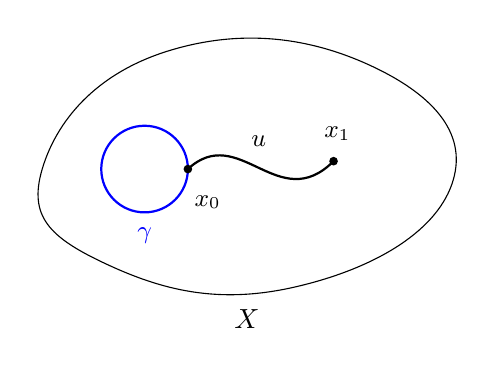
\begin{tikzpicture}[scale=1]
	\draw[thin] plot[smooth cycle, tension=0.8] coordinates {(-0.6,0.3) (1.0,1.8) (3.6,1.6) (4.6,0.1) (2.6,-1.2) (0.2,-0.9)};
	\node at (2.0,-1.6) {$X$};
	\draw[thick, color=blue] (0.7,0.3) circle (0.55);
	\node[color=blue] at (0.7,-0.55) {\small $\gamma$};
	\draw[thick] (1.25,0.3) .. controls (1.9,0.9) and (2.4,-0.3) .. (3.1,0.4);
	\node at (2.15,0.65) {\small $u$};
	\fill (1.25,0.3) circle (0.055); \node at (1.5,-0.12) {\small $x_0$};
	\fill (3.1,0.4) circle (0.055); \node at (3.15,0.75) {\small $x_1$};
\end{tikzpicture}
\end{center}

So if $x_0$ and $x_1$ are in the same path connected component, then
$\pi_1(X, x_0) \cong \pi_1(X, x_1)$. For a path connected space we will often write
$\pi_1(X)$, keeping in mind that the isomorphism depends on the choice of path, so this
is only well-defined up to (not necessarily inner) automorphism.

The next lemma is the technical heart of the section: it says that a homotopy between
maps which does \emph{not} respect basepoints still induces the same map on $\pi_1$,
provided we correct by the change of basepoint isomorphism along the track of the
basepoint.

\begin{lemma} \label{lem:homotopy-basepoint}
	Let $f, g: X \to Y$ be maps with $f \simeq_H g$, let $x_0 \in X$, and let $u(t) = H(x_0, t)$, a path $f(x_0) \leadsto g(x_0)$. Then the following diagram commutes.
	\[\begin{tikzcd}
		& {\pi_1(Y, f(x_0))} \\
		{\pi_1(X, x_0)} \\
		& {\pi_1(Y, g(x_0))}
		\arrow["{f_*}", from=2-1, to=1-2]
		\arrow["{u_\#}", from=1-2, to=3-2]
		\arrow["{g_*}"', from=2-1, to=3-2]
	\end{tikzcd}\]
	That is, $g_* = u_\# \circ f_*$.
\end{lemma}
\begin{proof}
	Suppose we have a loop $\gamma: I \rightarrow X$ based at $x_0$. We need to check that
	$$
	g_*([\gamma])=u_{\#} \circ f_*([\gamma]),
	$$
	in other words that
	$$
	g \circ \gamma \simeq u^{-1} \cdot(f \circ \gamma) \cdot u.
	$$
	To prove this we want to build a homotopy. Consider the composition
	$$
	F: I \times I \stackrel{\gamma \times \id_I}{\longrightarrow} X \times I \stackrel{H}{\longrightarrow} Y.
	$$
	Our plan is to exhibit two homotopic paths $\ell^{+}$ and $\ell^{-}$ in $I \times I$ such that
	$$
	F \circ \ell^{+}=g \circ \gamma, \qquad F \circ \ell^{-}=u^{-1} \cdot(f \circ \gamma) \cdot u.
	$$
	This is in general a good strategy: $X$ is a complicated and horrible space we do not understand, so to construct a homotopy we make ourselves work in the much nicer space $I \times I$.

	Our $\ell^{+}$ and $\ell^{-}$ are defined in a rather simple way. Precisely, $\ell^{+}$ is the path $s \mapsto(s, 1)$ along the top of the square, and $\ell^{-}$ is the concatenation of the paths $s \mapsto(0,1-s)$, $s \mapsto(s, 0)$ and $s \mapsto(1, s)$, going down the left edge, along the bottom, and up the right edge.
	\begin{center}
	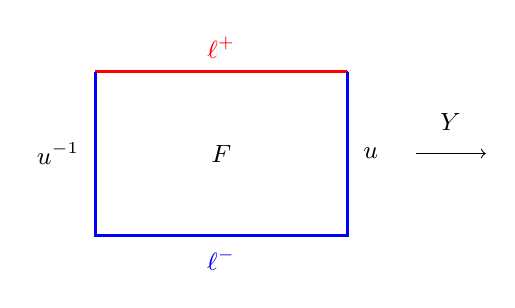
\begin{tikzpicture}[scale=1.6]
		\draw[thin] (0,0) rectangle (2,1.3);
		\draw[very thick, color=red] (0,1.3) -- (2,1.3);
		\draw[very thick, color=blue] (0,1.3) -- (0,0) -- (2,0) -- (2,1.3);
		\node[color=red, above] at (1,1.33) {\small $\ell^+$};
		\node[color=blue, below] at (1,-0.03) {\small $\ell^-$};
		\node[left] at (-0.05,0.65) {\small $u^{-1}$};
		\node[right] at (2.05,0.65) {\small $u$};
		\node at (1,0.65) {\small $F$};
		\draw[->] (2.55,0.65) -- (3.1,0.65);
		\node at (2.82,0.9) {\small $Y$};
	\end{tikzpicture}
	\end{center}
	Note that $\ell^{+}$ and $\ell^{-}$ are homotopic as paths. If this is not obvious, we can manually check the homotopy
	$$
	L(s, t)=t \ell^{+}(s)+(1-t) \ell^{-}(s),
	$$
	which works because $I \times I$ is convex, and fixes the endpoints $(0,1)$ and $(1,1)$. Hence $F \circ \ell^{+} \simeq F \circ \ell^{-}$ as paths, via $F \circ L$.

	Now we check that the compositions $F \circ \ell^{\pm}$ are indeed what we want. We have
	$$
	F \circ \ell^{+}(s)=H(\gamma(s), 1)=g \circ \gamma(s),
	$$
	and along the three pieces of $\ell^-$ we get $H(x_0, 1-s) = u^{-1}(s)$, then $H(\gamma(s), 0) = f(\gamma(s))$, then $H(x_0, s) = u(s)$, so that
	$$
	F \circ \ell^{-}=u^{-1} \cdot(f \circ \gamma) \cdot u
	$$
	as required.
\end{proof}

\begin{theorem} \label{thm:he-iso}
	If $f: X \rightarrow Y$ is a homotopy equivalence, and $x_0 \in X$, then the induced map
	$f_*: \pi_1(X, x_0) \rightarrow \pi_1(Y, f(x_0))$ is an isomorphism.
\end{theorem}
\begin{proof}
	Let $g: Y \rightarrow X$ be a homotopy inverse, so $f \circ g \simeq_H \id_Y$ and $g \circ f \simeq_{H^{\prime}} \id_X$.

	We have no guarantee that $g \circ f(x_0)=x_0$, but our homotopy $H'$ gives us a path $u^{\prime}=H^{\prime}(x_0, \cdot): x_0 \leadsto g \circ f(x_0)$.

	Applying Lemma \ref{lem:homotopy-basepoint} with $\id_X$ playing the role of `$f$' and $g \circ f$ playing the role of `$g$', we get
	$$
	u_{\#}^{\prime} \circ(\id_X)_*=(g \circ f)_*.
	$$
	Using functoriality, this says
	$$
	g_* \circ f_*=u_{\#}^{\prime}.
	$$
	However, we know that $u_{\#}^{\prime}$ is an isomorphism. So $f_*$ is injective and $g_*$ is surjective.

	Doing the same thing the other way round with $f \circ g$ instead of $g \circ f$, we learn that $g_*$ is injective and $f_*$ is surjective. So both are isomorphisms.
\end{proof}

This is a substantial improvement on Corollary \ref{cor:homeo-iso}: the fundamental group
cannot distinguish homotopy equivalent spaces, but that is exactly what makes it
computable, since we may replace a space by any convenient space homotopy equivalent to
it.

\begin{corollary}
	If $X$ is contractible, then $\pi_1(X, x_0)$ is trivial for every $x_0$.
\end{corollary}
\begin{proof}
	$\pi_1(*, *)$ is trivial, since there is only one loop, and $X \simeq *$.
\end{proof}

\subsection{Simply Connected Spaces}

\begin{definition}[Simply Connected Space]
	A space $X$ is \vocab{simply connected} if it is path connected and $\pi_1(X, x_0)$ is trivial for some (equivalently, by Proposition \ref{prop:change-basepoint}, any) choice of $x_0 \in X$.
\end{definition}

\begin{lemma} \label{lem:sc-unique-path}
	A path connected space $X$ is simply connected if and only if for any $x_0, x_1 \in X$, there is a unique homotopy class of paths $x_0 \leadsto x_1$.
\end{lemma}
\begin{proof}
	Suppose $X$ is simply connected, and let $u, v: x_0 \leadsto x_1$ be paths. Now $u \cdot v^{-1}$ is a loop based at $x_0$, so it is homotopic to the constant path. So we have
	$$
	u \simeq u \cdot v^{-1} \cdot v \simeq c_{x_0} \cdot v \simeq v.
	$$
	On the other hand, suppose there is a unique homotopy class of paths $x_0 \leadsto x_1$ for all $x_0, x_1 \in X$. Then in particular there is a unique homotopy class of loops based at $x_0$, namely that of $c_{x_0}$. So $\pi_1(X, x_0)$ is trivial.
\end{proof}

There is a useful reformulation of triviality in $\pi_1$ in terms of extending maps over
the disc. Recall that a loop $\gamma \in \Omega(X, x_0)$ has $\gamma(0) = \gamma(1)$, so
it descends to a map $\bar\gamma: S^1 \to X$ with $\bar{\gamma}(e^{2\pi i t}) = \gamma(t)$,
using $I/\{0,1\} \cong S^1$.

\begin{definition}
	A map $f: X \to Y$ is \vocab{null-homotopic} if $f \simeq c_p$ for some $p \in Y$.
\end{definition}

\begin{lemma} \label{lem:extend-disc}
	A map $f: S^1 \to Y$ extends to a map $F: D^2 \to Y$ if and only if $f$ is null-homotopic.
\end{lemma}
\begin{proof}
	If $F$ is such an extension, define $H(v, t) = F(tv)$ for $v \in S^1$. Then $H(v,1) = F(v) = f(v)$ and $H(v, 0) = F(0)$, so $f \simeq c_{F(0)}$.

	Conversely, suppose $f \simeq_H c_p$ with $H(v, 0) = p$ and $H(v,1) = f(v)$. Define
	$$
	F(v) = \begin{cases} H\!\left(\frac{v}{\norm{v}}, \norm{v}\right) & v \neq 0 \\ p & v = 0.\end{cases}
	$$
	This is continuous away from $0$, and continuous at $0$ because $H(w, t) \to p$ uniformly in $w$ as $t \to 0$ (using compactness of $S^1$). It restricts to $f$ on $S^1$.
\end{proof}

\begin{proposition} \label{prop:sc-equiv}
	For a path connected space $X$, the following are equivalent.
	\begin{enumerate}
		\item $X$ is simply connected.
		\item Every map $f: S^1 \to X$ is null-homotopic.
		\item Every map $f: S^1 \to X$ extends to a map $D^2 \to X$.
	\end{enumerate}
\end{proposition}
\begin{proof}
	Parts (ii) and (iii) are equivalent by Lemma \ref{lem:extend-disc}.

	Suppose $X$ is simply connected and let $f: S^1 \to X$, and set $x_0 = f(1)$ and $\gamma(t) = f(e^{2\pi i t})$, a loop at $x_0$ with $\bar\gamma = f$. Since $[\gamma] = 1$ we have $\gamma \simeq c_{x_0}$ via some $H$ fixing endpoints; then $\bar H(e^{2\pi i s}, t) = H(s,t)$ is well-defined (as $H(0,t) = H(1,t) = x_0$) and continuous, and gives $f \simeq c_{x_0}$.

	Conversely, suppose every map $S^1 \to X$ is null-homotopic and let $\gamma$ be a loop at $x_0$. Then $\bar\gamma$ extends to $F: D^2 \to X$, and $H(s,t) = F((1-t)e^{2\pi i s} + t)$ is a homotopy of paths from $\gamma$ to $c_{x_0}$: it takes the circle and shrinks it towards the basepoint $1 \in D^2$, staying inside $D^2$ by convexity, and it fixes $s = 0, 1$.
\end{proof}

\begin{example}
	Every convex subset of $\R^n$ is simply connected, being contractible. We will see in the next section that $S^1$ is \emph{not} simply connected, which is the first genuinely non-trivial computation of the course, and that $S^n$ for $n \geq 2$ \emph{is} simply connected.
\end{example}

\begin{example} \label{ex:pi1-product}
	If $X$ and $Y$ are spaces with basepoints $x_0, y_0$, then
	$$
	\pi_1(X \times Y, (x_0,y_0)) \cong \pi_1(X,x_0) \times \pi_1(Y,y_0).
	$$
	Indeed a map $I \to X \times Y$ is exactly a pair of maps $I \to X$ and $I \to Y$, by the universal property of the product topology, and likewise for homotopies $I \times I \to X\times Y$. So the two projections induce a bijection, which is clearly a homomorphism.
\end{example}

\section{Covering Spaces}

We now start to develop some machinery which will allow us to compute fundamental
groups. So far we have no example of a space with a non-trivial fundamental group, for
the good reason that showing a loop is \emph{not} null-homotopic means ruling out all
possible homotopies at once. The trick is to unroll the space: if we can find a
simply connected space sitting above $X$ in a suitably uniform way, then loops in $X$
become paths upstairs, and paths are much easier to tell apart than loops.

\subsection{Definitions and Examples}

\begin{definition}[Evenly Covered Set]
	Suppose $p: \hat{X} \rightarrow X$ is a map. We say that an open set $U \subseteq X$ is \vocab{evenly covered} by $p$ if
	$$
	p^{-1}(U)=\bigsqcup_{\alpha \in A} V_\alpha,
	$$
	a disjoint union of open sets, where $p|_{V_\alpha}: V_\alpha \rightarrow U$ is a homeomorphism for each $\alpha \in A$.
\end{definition}

The $V_\alpha$ are called the \vocab{sheets} over $U$. Note that the inverse
$p_\alpha^{-1} = (p|_{V_\alpha})^{-1}: U \to \hat X$ is continuous, being the inverse of
a homeomorphism followed by an inclusion; we will use this constantly.

\begin{definition}[Covering Map]
	A map $p: \hat{X} \rightarrow X$ is a \vocab{covering map} if for all $x \in X$ there exists an open neighbourhood $U_x$ of $x$ which is evenly covered by $p$. In this case, we call $\hat{X}$ a \vocab{covering space} for $X$.
\end{definition}

\begin{center}
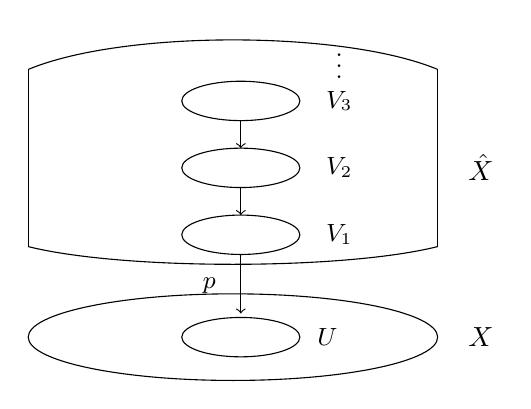
\begin{tikzpicture}[scale=1]
	% base
	\draw[thin] (0,0) ellipse (2.6 and 0.55);
	\node at (3.15,0) {$X$};
	\draw[thin] (0.1,0) ellipse (0.75 and 0.25);
	\node at (1.2,0) {\small $U$};
	% sheets
	\foreach \y in {1.3, 2.15, 3.0} {
		\draw[thin] (0.1,\y) ellipse (0.75 and 0.25);
	}
	\node at (1.35,1.3) {\small $V_1$};
	\node at (1.35,2.15) {\small $V_2$};
	\node at (1.35,3.0) {\small $V_3$};
	\node at (1.35,3.55) {\small $\vdots$};
	\node at (3.15,2.15) {$\hat X$};
	\draw[thin] (-2.6,1.15) -- (-2.6,3.4);
	\draw[thin] (2.6,1.15) -- (2.6,3.4);
	\draw[thin] (-2.6,3.4) .. controls (-1.4,3.9) and (1.4,3.9) .. (2.6,3.4);
	\draw[thin] (-2.6,1.15) .. controls (-1.4,0.85) and (1.4,0.85) .. (2.6,1.15);
	% projection arrows
	\draw[->, thin] (0.1,1.05) -- (0.1,0.3);
	\draw[->, thin] (0.1,1.9) -- (0.1,1.55);
	\draw[->, thin] (0.1,2.75) -- (0.1,2.4);
	\node at (-0.3,0.65) {\small $p$};
\end{tikzpicture}
\end{center}

\begin{example}
	Let $A$ be a set with the discrete topology. Then the projection $p: A \times X \to X$ is a covering map, since $X$ itself is evenly covered: $p^{-1}(X) = \bigsqcup_{\alpha \in A} \{\alpha\} \times X$. This is the \vocab{trivial cover}, and the point of the definition is that a general covering map looks like this \emph{locally} but need not do so globally.
\end{example}

\begin{example} \label{ex:helix}
	The map $p: \R \to S^1$ given by $p(t) = e^{2\pi i t}$ is a covering map. Indeed, if $V \subseteq \R$ is an open interval of length less than $1$ and $U = p(V)$, then
	$$
	p^{-1}(U) = \bigsqcup_{n \in \Z} (V + n),
	$$
	and $p$ restricted to each translate $V + n$ is a homeomorphism onto $U$. Every point of $S^1$ has such a neighbourhood.
\end{example}

The picture to have in mind is the helix: $\R$ winds around and around above the circle,
and $p$ is vertical projection.

\begin{center}
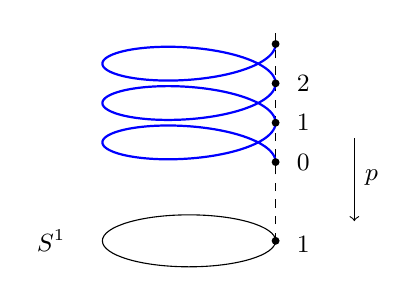
\begin{tikzpicture}[scale=1]
	% fibre
	\draw[thin, dashed] (1.1,-1.0) -- (1.1,1.7);
	% helix
	\draw[thick, color=blue, samples=300, domain=0:1080, smooth, variable=\t]
		plot ({1.1*cos(\t)}, {0.33*sin(\t) + \t/720});
	\node[color=blue] at (-1.75,1.15) {\small $\R$};
	% circle
	\draw[thin] (0,-1.0) ellipse (1.1 and 0.33);
	\node at (-1.75,-1.0) {\small $S^1$};
	% marked fibre points
	\foreach \y in {0, 0.5, 1.0, 1.5} { \fill (1.1,\y) circle (0.05); }
	\node at (1.45,0) {\small $0$};
	\node at (1.45,0.5) {\small $1$};
	\node at (1.45,1.0) {\small $2$};
	\fill (1.1,-1.0) circle (0.05);
	\node at (1.45,-1.05) {\small $1$};
	% projection
	\draw[->, thin] (2.1,0.3) -- (2.1,-0.75);
	\node at (2.32,-0.2) {\small $p$};
\end{tikzpicture}
\end{center}

\begin{example} \label{ex:zn-cover}
	For $n \geq 1$, the map $p_n: S^1 \to S^1$, $z \mapsto z^n$, is a covering map. If $U \subseteq S^1$ is an open arc of length less than $2\pi/n$ then
	$$
	p_n^{-1}(U) = \bigsqcup_{i \in \Z/n\Z} \omega^i V, \qquad \omega = e^{2\pi i /n},
	$$
	where $V$ is one of the $n$ arcs mapping homeomorphically onto $U$. So this is an $n$-sheeted cover.
\end{example}

\begin{definition}
	The \vocab{$n$-dimensional real projective space} is $\RP^n = S^n/\!\sim$, where $\sim$ is generated by $x \sim -x$, with the quotient topology.
\end{definition}

\begin{example} \label{ex:rpn-cover}
	The quotient map $p: S^n \to \RP^n$ is a covering map. Given $x \in S^n$, let $V_x$ be the open hemisphere centred at $x$ and $U_x = p(V_x)$. Since $V_x$ contains no pair of antipodal points, $p^{-1}(U_x) = V_x \sqcup (-V_x)$ and $p$ restricted to each is a homeomorphism onto $U_x$. This is a two-sheeted cover.
\end{example}

\begin{example} \label{ex:torus-cover}
	The map $p \times p: \R^2 \to S^1 \times S^1 = T^2$ is a covering map of the torus, being a product of covering maps.
\end{example}

\subsection{Lifting}

The whole theory rests on the following idea: given a map into $X$, we try to push it up
into $\hat X$.

\begin{definition}[Lift]
	Suppose $p: \hat{X} \rightarrow X$ is a covering map and $f: Z \rightarrow X$ is a map. Then we say that $\hat{f}: Z \rightarrow \hat{X}$ is a \vocab{lift} of $f$ if $p \circ \hat{f}=f$, that is, if
	\[\begin{tikzcd}
		& {\hat X} \arrow[d, "p"] \\
		Z \arrow[ru, "{\hat f}", dashed] \arrow[r, "f"'] & X
	\end{tikzcd}\]
	commutes.
\end{definition}

\begin{notation}
	We say a map $f: Z \to X$ has the \vocab{lifting property} at $z_0 \in Z$ if for every $\hat{x}_0 \in p^{-1}(f(z_0))$ there is a lift $\hat f$ of $f$ with $\hat{f}(z_0) = \hat{x}_0$, and the \vocab{unique lifting property} (ULP) at $z_0$ if this lift is moreover unique. For a path $\gamma: [a,b] \to X$ we say `$\gamma$ has the ULP' to mean that it has the ULP at $a$.
\end{notation}

The strategy for lifting a path is to chop it into small pieces, each of which lands in a
single evenly covered set, and lift those one at a time. To chop it up we need the
following, which the reader may have seen in a metric spaces course.

\begin{lemma}[Lebesgue Covering Lemma] \label{lem:lebesgue}
	Suppose $X$ is a compact metric space and $\left\{U_\alpha\right\}_\alpha$ is an open cover of $X$. Then there exists $\delta>0$ such that for all $x \in X$ we have $B_\delta(x) \subseteq U_\alpha$ for some $\alpha$.
\end{lemma}
\begin{proof}
	Given $x \in X$, let $\alpha(x)$ and $\delta(x)>0$ be such that $B_{2 \delta(x)}(x) \subseteq U_{\alpha(x)}$. Then $\{B_{\delta(x)}(x)\}_{x \in X}$ is an open cover of $X$, so by compactness there is a finite subcover $\{B_{\delta(x_i)}(x_i)\}_{i=1}^n$. Let $\delta=\min \{\delta(x_1), \ldots, \delta(x_n)\}>0$. Then given $y \in X$ we have $y \in B_{\delta(x_i)}(x_i)$ for some $i$, and so
	$$
	B_\delta(y) \subseteq B_{\delta(x_i) + \delta}(x_i) \subseteq B_{2 \delta(x_i)}(x_i) \subseteq U_{\alpha(x_i)}
	$$
	as required.
\end{proof}

\begin{lemma} \label{lem:lift-small}
	Let $f: Z \to X$ with $Z$ connected, and suppose $\operatorname{im}(f) \subseteq U$ where $U$ is evenly covered. Then $f$ has the unique lifting property at every $z_0 \in Z$.
\end{lemma}
\begin{proof}
	Since $U$ is evenly covered, $p^{-1}(U)=\bigsqcup_\alpha V_\alpha$. Given $\hat x_0 \in p^{-1}(f(z_0))$ we have $\hat{x}_0 \in V_{\alpha_0}$ for some $\alpha_0$. Then $p_{\alpha_0}^{-1} = (p|_{V_{\alpha_0}})^{-1}: U \rightarrow \hat{X}$ is continuous with $p_{\alpha_0}^{-1}(f(z_0))=\hat{x}_0$, so $\hat{f}=p_{\alpha_0}^{-1} \circ f$ is a lift of $f$ with the right value at $z_0$.

	For uniqueness, notice that $p^{-1}(U)=V_{\alpha_0} \sqcup(\bigsqcup_{\alpha \neq \alpha_0} V_\alpha)$ is a disconnection of $p^{-1}(U)$. Any lift $\hat f$ has connected image (as $Z$ is connected) meeting $V_{\alpha_0}$, so $\operatorname{im}(\hat{f}) \subseteq V_{\alpha_0}$. But $p|_{V_{\alpha_0}}$ is a homeomorphism, so $\hat f = p_{\alpha_0}^{-1} \circ f$ is forced.
\end{proof}

\begin{lemma} \label{lem:lift-glue}
	Suppose $\gamma:[a, b] \rightarrow X$ and $a^{\prime} \in[a, b]$. If $\gamma|_{[a, a^{\prime}]}$ has the ULP at $a$ and $\gamma|_{[a^{\prime}, b]}$ has the ULP at $a^{\prime}$, then $\gamma$ has the ULP at $a$.
\end{lemma}
\begin{proof}
	Given $\hat x \in p^{-1}(\gamma(a))$, we have a lift $\hat{\gamma}_1:[a, a^{\prime}] \rightarrow \hat{X}$ of $\gamma|_{[a, a^{\prime}]}$ with $\hat\gamma_1(a) = \hat x$, and then a lift $\hat{\gamma}_2:[a^{\prime}, b] \rightarrow \hat{X}$ of $\gamma|_{[a^{\prime}, b]}$ with $\hat{\gamma}_2(a^{\prime})=\hat{\gamma}_1(a^{\prime})$. So the concatenation $\hat{\gamma}_1 \hat{\gamma}_2$, which is continuous by the gluing lemma, is a lift of $\gamma$ at $a$.

	For uniqueness, suppose $\hat{\eta}$ is any lift with $\hat\eta(a) = \hat x$. Then $\hat{\eta}|_{[a, a^{\prime}]}$ is a lift of $\gamma|_{[a, a^{\prime}]}$ starting at $\hat x$, so $\hat{\eta}|_{[a, a^{\prime}]}=\hat{\gamma}_1$ by uniqueness. In particular $\hat\eta(a') = \hat\gamma_1(a')$, so $\hat\eta|_{[a',b]} = \hat\gamma_2$ by uniqueness again. Hence $\hat\eta = \hat\gamma_1\hat\gamma_2$.
\end{proof}

\begin{theorem}[Path Lifting] \label{thm:path-lifting}
	Let $p: \hat X \to X$ be a covering map. Then any path $\gamma: I \rightarrow X$ has the unique lifting property.
\end{theorem}
\begin{proof}
	Since $p$ is a covering map, every $x \in X$ has an evenly covered neighbourhood $U_x$. Then $\{U_x \mid x \in X\}$ is an open cover of $X$, so $\{\gamma^{-1}(U_x) \mid x \in X\}$ is an open cover of $I$. Thus by the Lebesgue covering lemma there exists $\delta>0$ such that for each $t$ we have $B_\delta(t) \subseteq \gamma^{-1}(U_{x(t)})$ for some $x(t)$.

	Choose $n$ with $1/n<\delta$ and set $a_i=i/n$. Then $[a_i, a_{i+1}] \subseteq B_\delta(a_i)$, so $\gamma([a_i, a_{i+1}]) \subseteq U_{x(a_i)}$, which is evenly covered. As $[a_i,a_{i+1}]$ is connected, Lemma \ref{lem:lift-small} says $\gamma|_{[a_i, a_{i+1}]}$ has the ULP at $a_i$. By induction on $i$ using Lemma \ref{lem:lift-glue}, $\gamma|_{[0,a_i]}$ has the ULP at $0$ for every $i$, and in particular so does $\gamma$.
\end{proof}

The same argument, run over a grid of small squares instead of a partition of the
interval, lifts homotopies.

\begin{theorem}[Homotopy Lifting] \label{thm:homotopy-lifting}
	Suppose $p: \hat{X} \rightarrow X$ is a covering map and $H: I \times I \rightarrow X$ is a homotopy. Then $H$ has the lifting property at $(0,0)$.
\end{theorem}
\begin{proof}
	Let $\{U_x \mid x \in X\}$ be an open cover of $X$ by evenly covered neighbourhoods. Since $I^2$ is compact, by the Lebesgue covering lemma there exists $\delta>0$ such that $B_\delta(v) \subseteq H^{-1}(U_{x(v)})$ for each $v \in I^2$.

	Choose $n$ with $\sqrt{2}/n<\delta$ and divide $I^2$ into squares of side length $1/n$. Enumerate them $A_1, A_2, \ldots, A_{n^2}$, starting from the bottom left and going right along each row and then up. Label the bottom left corner of $A_i$ as $v_i$, so that $v_1 = (0,0)$. Since $A_i \subseteq B_\delta(v_i)$ we have $H(A_i) \subseteq U_{x(v_i)}$, which is evenly covered, and $A_i$ is connected, so $H|_{A_i}$ has the ULP at $v_i$ by Lemma \ref{lem:lift-small}. Let $B_k=\bigcup_{i=1}^k A_i$.

	\begin{center}
	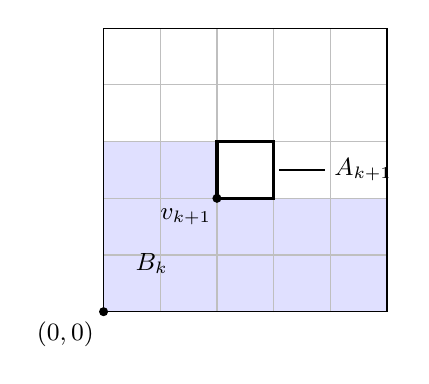
\begin{tikzpicture}[scale=0.72]
		\fill[color=blue!12] (0,0) rectangle (5,2);
		\fill[color=blue!12] (0,2) rectangle (2,3);
		\draw[color=lightgray, thin] (0,0) grid (5,5);
		\draw[thin] (0,0) rectangle (5,5);
		\draw[very thick] (2,2) rectangle (3,3);
		\draw[thin] (3.1,2.5) -- (3.9,2.5);
		\node[right] at (3.9,2.5) {\small $A_{k+1}$};
		\fill (2,2) circle (0.08);
		\node at (1.45,1.68) {\small $v_{k+1}$};
		\node at (0.85,0.85) {\small $B_k$};
		\fill (0,0) circle (0.08);
		\node[below left] at (0,0) {\small $(0,0)$};
	\end{tikzpicture}
	\end{center}

	We prove by induction that $H|_{B_k}$ has the lifting property at $(0,0)$. For $k=1$ we have $B_1=A_1$ and $v_1 = (0,0)$, so this is what we already know. Now suppose $H|_{B_k}$ has a lift $\hat{H}_k: B_k \rightarrow \hat X$ with $\hat{H}_k(0,0)=\hat{x}$. As $H|_{A_{k+1}}$ has the lifting property at $v_{k+1}$, we may choose a lift $\hat{h}_k: A_{k+1} \rightarrow \hat{X}$ with $\hat{h}_k(v_{k+1})=\hat{H}_k(v_{k+1})$.

	Now $B_k \cap A_{k+1}$ is either one or two edges of $A_{k+1}$, in either case a set homeomorphic to $I$ containing $v_{k+1}$. By uniqueness of path lifting, $\hat{H}_k$ and $\hat h_k$ agree on $A_{k+1} \cap B_k$, since both are lifts of $H|_{A_{k+1}\cap B_k}$ agreeing at $v_{k+1}$. So by the gluing lemma we obtain a well-defined lift $\hat{H}_{k+1}$ of $H|_{B_{k+1}}$. Taking $k = n^2$ finishes the proof.
\end{proof}

The point of all this is the following, which says that homotopic loops downstairs lift to
paths with the same endpoint upstairs. This is the mechanism that will let us distinguish
loops.

\begin{proposition} \label{prop:lift-homotopic}
	Let $p: \hat X \to X$ be a covering map and suppose $\gamma_0, \gamma_1 \in \Omega\left(X, x_0, x_1\right)$ with $\gamma_0 \simeq \gamma_1$. Let $\hat{\gamma}_i$ be the lift of $\gamma_i$ with $\hat{\gamma}_i(0)=\hat{x}_0$. Then $\hat{\gamma}_0 \simeq \hat{\gamma}_1$. In particular, $\hat{\gamma}_0(1)=\hat{\gamma}_1(1)$.
\end{proposition}
\begin{proof}
	Suppose $H: I^2 \rightarrow X$ is a homotopy of paths between $\gamma_0$ and $\gamma_1$. By homotopy lifting we have a lift $\hat{H}: I^2 \rightarrow \hat{X}$ with $\hat{H}(0,0)=\hat{x}_0$. Let $\alpha_i(t)=\hat{H}(t, i)$ and $\beta_i(t)=\hat{H}(i, t)$ for $i = 0,1$, the images of the four edges of the square.
	\begin{center}
	\begin{tikzpicture}[scale=1.5]
		\draw[thin] (0,0) rectangle (2,1.3);
		\node[below] at (1,-0.03) {\small $\alpha_0$};
		\node[above] at (1,1.33) {\small $\alpha_1$};
		\node[left] at (-0.05,0.65) {\small $\beta_0$};
		\node[right] at (2.05,0.65) {\small $\beta_1$};
		\node at (1,0.65) {\small $\hat H$};
		\fill (0,0) circle (0.03); \node at (-0.25,-0.05) {\small $\hat x_0$};
	\end{tikzpicture}
	\end{center}
	Applying uniqueness of path lifting to each edge in turn:
	\begin{enumerate}
		\item $\beta_0$ is a lift of the constant path $c_{x_0}$ starting at $\hat x_0$, so $\beta_0 = c_{\hat x_0}$;
		\item $\alpha_0$ is a lift of $\gamma_0$ with $\alpha_0(0) = \hat x_0$, so $\alpha_0 = \hat\gamma_0$;
		\item $\alpha_1$ is a lift of $\gamma_1$ with $\alpha_1(0) = \beta_0(1) = \hat x_0$, so $\alpha_1 = \hat\gamma_1$;
		\item writing $\hat x_1 = \hat\gamma_0(1)$, $\beta_1$ is a lift of $c_{x_1}$ starting at $\hat x_1$, so $\beta_1 = c_{\hat x_1}$.
	\end{enumerate}
	So $\hat H$ is a homotopy of paths from $\hat\gamma_0$ to $\hat\gamma_1$, and in particular the two have the same endpoint $\hat x_1$.
\end{proof}

\begin{corollary} \label{cor:p-injective}
	If $p: (\hat X, \hat x_0) \to (X, x_0)$ is a covering map, then $p_*: \pi_1(\hat{X}, \hat{x}_0) \rightarrow \pi_1(X, x_0)$ is injective.
\end{corollary}
\begin{proof}
	Suppose $p_*[\gamma_0] = p_*[\gamma_1]$ for loops $\gamma_0, \gamma_1$ at $\hat x_0$. Then $p \circ \gamma_0 \simeq p \circ \gamma_1$ as paths, so by Proposition \ref{prop:lift-homotopic} their lifts starting at $\hat x_0$ are homotopic as paths. But these lifts are $\gamma_0$ and $\gamma_1$, by uniqueness of lifting. So $[\gamma_0] = [\gamma_1]$.
\end{proof}

\subsection{The Fundamental Group of the Circle}

Fix a covering map $p: (\hat X, \hat x_0) \to (X, x_0)$. Given a loop $\gamma$ at $x_0$,
let $\hat\gamma$ be its unique lift starting at $\hat x_0$. Then
$p(\hat\gamma(1)) = \gamma(1) = x_0$, so $\hat\gamma(1)$ lies in the \vocab{fibre}
$p^{-1}(x_0)$, and by Proposition \ref{prop:lift-homotopic} it depends only on the
homotopy class of $\gamma$. We therefore get a well-defined function
$$
\varepsilon_p: \pi_1(X, x_0) \longrightarrow p^{-1}(x_0), \qquad [\gamma] \mapsto \hat\gamma(1).
$$
This is the key construction: it turns a homotopy-theoretic object into a set of points.

\begin{definition}[Universal Cover]
	A covering map $p: \hat{X} \to X$ is a \vocab{universal cover} if $\hat X$ is simply connected.
\end{definition}

\begin{example}
	$p: \R \to S^1$, $t \mapsto e^{2\pi i t}$, is a universal cover, since $\R$ is contractible. Likewise $\R^2 \to T^2$ is a universal cover of the torus.
\end{example}

\begin{proposition} \label{prop:eps-bijection}
	If $p: (\hat X, \hat x_0) \to (X, x_0)$ is a universal cover, then $\varepsilon_p: \pi_1(X, x_0) \to p^{-1}(x_0)$ is a bijection.
\end{proposition}
\begin{proof}
	\emph{Injectivity.} Suppose $\varepsilon_p[\gamma_0] = \varepsilon_p[\gamma_1] = \hat x_1$. Then $\hat\gamma_0$ and $\hat\gamma_1$ are both paths from $\hat x_0$ to $\hat x_1$ in $\hat X$, which is simply connected, so $\hat\gamma_0 \simeq \hat\gamma_1$ as paths by Lemma \ref{lem:sc-unique-path}. Composing the homotopy with $p$ gives $\gamma_0 \simeq \gamma_1$, so $[\gamma_0] = [\gamma_1]$.

	\emph{Surjectivity.} Given $\hat x \in p^{-1}(x_0)$, use path connectedness of $\hat X$ to find a path $\eta: \hat x_0 \leadsto \hat x$. Then $\gamma = p \circ \eta$ is a loop at $x_0$, and $\eta$ is its lift starting at $\hat x_0$, so $\varepsilon_p[\gamma] = \eta(1) = \hat x$.
\end{proof}

This is already enough to compute the fundamental group of the circle as a \emph{set}: we
have $p^{-1}(1) = \Z$ for the helix covering, so $\pi_1(S^1, 1)$ is countably infinite. To
get the group structure we have to work slightly harder, and the mechanism is that we
can slide the covering space $\R$ along itself.

\begin{theorem} \label{thm:pi1-circle}
	$\varepsilon_p: \pi_1(S^1, 1) \to \Z$ is a group isomorphism. In particular $\pi_1(S^1) \cong \Z$.
\end{theorem}
\begin{proof}
	It is a bijection by Proposition \ref{prop:eps-bijection}, using $p^{-1}(1) = \Z \subseteq \R$, so it suffices to check that it is a homomorphism.

	For $n \in \Z$ define $\varphi_n: \R \to \R$ by $\varphi_n(x) = x + n$. Then $p \circ \varphi_n = p$, since $e^{2\pi i (x+n)} = e^{2\pi i x}$. So if $\hat\gamma$ is any lift of a path $\gamma$, then $\varphi_n \circ \hat\gamma$ is another lift, now starting at $\hat\gamma(0) + n$.

	Suppose $\varepsilon_p[\gamma] = n$ and $\varepsilon_p[\gamma'] = n'$, so the lifts based at $0$ satisfy $\hat\gamma(1) = n$ and $\hat{\gamma'}(1) = n'$. Then $\varphi_n \circ \hat{\gamma'}$ is a lift of $\gamma'$ starting at $n = \hat\gamma(1)$, so the concatenation
	$$
	\widehat{\gamma \cdot \gamma'} = \hat\gamma \cdot (\varphi_n \circ \hat{\gamma'})
	$$
	is the lift of $\gamma \cdot \gamma'$ starting at $0$. Evaluating at $1$,
	$$
	\varepsilon_p[\gamma\cdot\gamma'] = \varphi_n(\hat{\gamma'}(1)) = n + n' = \varepsilon_p[\gamma] + \varepsilon_p[\gamma'].
	$$
	So $\varepsilon_p$ is a homomorphism, and hence an isomorphism.
\end{proof}

Concretely, the class corresponding to $n \in \Z$ is that of the loop
$\gamma_n(t) = e^{2\pi i n t}$, which winds $n$ times around the circle: its lift starting
at $0$ is $\hat\gamma_n(t) = nt$, ending at $n$. So the fundamental group of the circle
counts winding number, exactly as intuition demands.

\begin{corollary}
	$S^1$ is not contractible, and $S^1$ is not a retract of $D^2$.
\end{corollary}
\begin{proof}
	If $S^1$ were contractible then $\pi_1(S^1)$ would be trivial, but it is $\Z$.

	Suppose $r: D^2 \to S^1$ were a retraction, with $\iota: S^1 \hookrightarrow D^2$ the inclusion. Then $r \circ \iota = \id_{S^1}$, so $r_* \circ \iota_* = \id$ on $\pi_1(S^1, 1) = \Z$. But $\iota_*$ factors through $\pi_1(D^2, 1)$, which is trivial as $D^2$ is convex. So the identity on $\Z$ factors through the trivial group, which is absurd.
\end{proof}

\begin{corollary}[Brouwer Fixed Point Theorem, $n=2$]
	Every map $f: D^2 \to D^2$ has a fixed point.
\end{corollary}
\begin{proof}
	Suppose $f(x) \neq x$ for all $x$. Define $r(x) \in S^1$ to be the point where the ray from $f(x)$ through $x$ meets $S^1$. This is continuous (we will verify a formula for it in Theorem \ref{thm:brouwer}), and if $x \in S^1$ then $r(x) = x$. So $r$ is a retraction $D^2 \to S^1$, contradicting the previous corollary.
\end{proof}

\begin{example} \label{ex:pi1-torus}
	Since $\pi_1(X \times Y) \cong \pi_1(X) \times \pi_1(Y)$ (Example \ref{ex:pi1-product}), the torus has
	$$
	\pi_1(T^2) = \pi_1(S^1 \times S^1) \cong \Z^2 .
	$$
	This already tells us that $T^2 \not\simeq S^2$ once we know that $S^2$ is simply connected, and that $T^2 \not\simeq S^1 \vee S^1$ once we know the latter has non-abelian fundamental group.
\end{example}

\subsection{Degree and the Fundamental Theorem of Algebra}

The isomorphism $\pi_1(S^1) \cong \Z$ lets us attach an integer to any self-map of the
circle. There is one small nuisance: a map $f: S^1 \to S^1$ need not preserve the
basepoint, so $f_*$ lands in $\pi_1(S^1, f(1))$ rather than $\pi_1(S^1, 1)$. We fix this
by transporting back along a path, and the following lemma says that the choice of path
does not matter.

\begin{lemma} \label{lem:degree-welldefined}
	Let $z \in S^1$ and let $u, v: z \leadsto 1$ be paths. Then $u_\# = v_\#: \pi_1(S^1, z) \to \pi_1(S^1, 1)$.
\end{lemma}
\begin{proof}
	By Proposition \ref{prop:change-basepoint}, $(v^{-1})_\# \circ u_\#$ is the map $[\gamma] \mapsto [\eta][\gamma][\eta]^{-1}$ where $\eta = v \cdot u^{-1}$ is a loop at $1$. But $\pi_1(S^1, 1) \cong \Z$ is abelian, so conjugation is trivial and $(v^{-1})_\# \circ u_\# = \id$. Hence $u_\# = v_\#$.
\end{proof}

\begin{definition}[Degree]
	Let $f: S^1 \to S^1$ be a map, and set $z = f(1)$. Choose any path $u: z \leadsto 1$. Then
	$$
	u_\# \circ f_*: \pi_1(S^1,1) \to \pi_1(S^1,1)
	$$
	is a homomorphism $\Z \to \Z$, so is multiplication by some integer. We define the \vocab{degree} $\deg f$ to be that integer, namely $(u_\# \circ f_*)(1)$.
\end{definition}

By Lemma \ref{lem:degree-welldefined} this is independent of the choice of $u$.
Intuitively, $\deg f$ counts how many times $f$ wraps the circle around itself, with sign.

\begin{center}
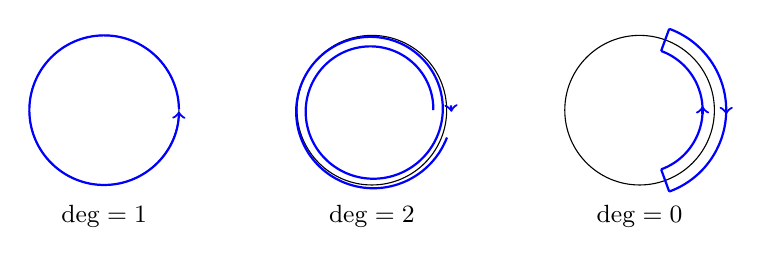
\begin{tikzpicture}[scale=1]
	\draw[thin] (0,0) circle (0.95);
	\draw[->, thick, color=blue] (0.8:0.95) arc (0.8:359:0.95);
	\node at (0,-1.35) {\small $\deg = 1$};
	\begin{scope}[xshift=3.4cm]
		\draw[thin] (0,0) circle (0.95);
		\draw[thick, color=blue, samples=250, domain=0:700, smooth, variable=\t]
			plot ({(0.78 + 0.00033*\t)*cos(\t)}, {(0.78+0.00033*\t)*sin(\t)});
		\draw[->, thick, color=blue] (1.005,0.06) -- (1.01,-0.02);
		\node at (0,-1.35) {\small $\deg = 2$};
	\end{scope}
	\begin{scope}[xshift=6.8cm]
		\draw[thin] (0,0) circle (0.95);
		\draw[thick, color=blue] (-70:0.8) arc (-70:70:0.8);
		\draw[thick, color=blue] (-70:1.1) arc (-70:70:1.1);
		\draw[thick, color=blue] (70:0.8) -- (70:1.1);
		\draw[thick, color=blue] (-70:0.8) -- (-70:1.1);
		\draw[->, thick, color=blue] (0.8,-0.05) -- (0.8,0.05);
		\draw[->, thick, color=blue] (1.1,0.05) -- (1.1,-0.05);
		\node at (0,-1.35) {\small $\deg = 0$};
	\end{scope}
\end{tikzpicture}
\end{center}

\begin{proposition} \label{prop:degree}
	Let $f_n: S^1 \to S^1$ be given by $z \mapsto z^n$. Then
	\begin{enumerate}
		\item $\deg f_n = n$;
		\item maps $g_0, g_1: S^1 \to S^1$ are homotopic if and only if $\deg g_0 = \deg g_1$;
		\item $g: S^1 \to S^1$ extends to a map $D^2 \to S^1$ if and only if $\deg g = 0$.
	\end{enumerate}
\end{proposition}
\begin{proof}
	(i) Since $f_n(1) = 1$ we may take $u$ constant. Now $f_n \circ \gamma_1 = \gamma_n$, where $\gamma_n(t) = e^{2\pi int}$, so $f_{n*}[\gamma_1] = [\gamma_n]$, which corresponds to $n \in \Z$.

	(ii) Suppose $g_0 \simeq_H g_1$, and let $u(t) = H(1,t)$, a path $g_0(1) \leadsto g_1(1)$. By Lemma \ref{lem:homotopy-basepoint}, $g_{1*} = u_\# \circ g_{0*}$. Choose $v: g_1(1) \leadsto 1$; then $u \cdot v : g_0(1) \leadsto 1$ and
	$$
	\deg g_1 = (v_\# \circ g_{1*})(1) = (v_\# \circ u_\# \circ g_{0*})(1) = ((u\cdot v)_\# \circ g_{0*})(1) = \deg g_0,
	$$
	using $(u \cdot v)_\# = v_\# \circ u_\#$.

	Conversely, it is enough to show $g \simeq f_{\deg g}$. First suppose $g(1) = 1$, and let $\gamma = g \circ \gamma_1$, so that $g = \bar\gamma$ and $\deg g = g_*(1) = [\gamma]$. If $\deg g = n$ then $\gamma \simeq \gamma_n$ as paths, whence $\bar\gamma \simeq \bar\gamma_n = f_n$ as maps $S^1 \to S^1$. In general, if $g(1) = e^{2\pi i x}$, then $g \simeq g_0$ where $g_0(z) = e^{-2\pi i x}g(z)$, via the homotopy $g_t(z) = e^{-2\pi i tx}g(z)$; and $g_0(1) = 1$, so we may apply the previous case.

	(iii) By Lemma \ref{lem:extend-disc}, $g$ extends to $D^2$ if and only if $g$ is null-homotopic, that is, if and only if $g \simeq c_{1} = f_0$, which by (ii) happens if and only if $\deg g = 0$.
\end{proof}

As an application, we can now prove the fundamental theorem of algebra --- a statement
with no topology in it whatsoever --- by a winding number argument.

Let $P(w) = w^n + a_{n-1}w^{n-1} + \dots + a_0 = w^n + q(w)$ be a monic complex polynomial
of degree $n \geq 1$.

\begin{lemma} \label{lem:fta-bound}
	Let $R_0 = \max\{1, \sum_{i=0}^{n-1}|a_i|\}$. Then $|w| > R_0$ implies $|w^n| > |q(w)|$.
\end{lemma}
\begin{proof}
	If $|w| > R_0 \geq 1$ then $|w|^{i - n + 1} \leq 1$ for $0 \leq i \leq n-1$, so
	$$
	\frac{|q(w)|}{|w|^{n-1}} \leq \sum_{i=0}^{n-1} |a_i| |w|^{i-n+1} \leq \sum_{i=0}^{n-1}|a_i| \leq R_0.
	$$
	Dividing by $|w|$ gives $|q(w)|/|w|^n \leq R_0/|w| < 1$.
\end{proof}

\begin{theorem}[Fundamental Theorem of Algebra]
	Every complex polynomial of degree $n \geq 1$ has a root in $\C$.
\end{theorem}
\begin{proof}
	We may assume $P$ is monic, as above. Fix $R > R_0$ and consider the two maps $g_0, g_1: S^1 \to \C \setminus \{0\}$ given by
	$$
	g_0(z) = (Rz)^n, \qquad g_1(z) = P(Rz).
	$$
	These are homotopic via $g_t(z) = P_t(Rz)$ where $P_t(w) = w^n + t q(w)$: this really does avoid $0$, since $|w| = R > R_0$ gives $|w^n| > |q(w)| \geq |tq(w)|$ by Lemma \ref{lem:fta-bound}. Let $\pi: \C \setminus \{0\} \to S^1$ be the radial projection $w \mapsto w/|w|$. Then $\pi \circ g_0 \simeq \pi \circ g_1$ as maps $S^1 \to S^1$, and $\pi \circ g_0 = f_n$ up to the constant $R^n/|R^n|=1$, so
	$$
	\deg(\pi \circ g_1) = \deg (\pi \circ g_0) = n.
	$$
	Now suppose for contradiction that $P$ has no root. Then $P: \C \to \C\setminus\{0\}$, so $g_1$ extends to $G_1: D^2 \to \C \setminus \{0\}$ by $G_1(z) = P(Rz)$, and hence $\pi \circ g_1$ extends to $\pi \circ G_1: D^2 \to S^1$. By Proposition \ref{prop:degree}(iii) this forces $\deg (\pi\circ g_1) = 0$, so $n = 0$, contradicting $n \geq 1$.
\end{proof}

\subsection{The Lifting Criterion}

We can lift paths and homotopies. When can we lift a map from a general space $Z$? There
are two obstructions, one of which we have already met.

\begin{definition}
	A space $X$ is \vocab{locally path connected} if for every open $U \subseteq X$ and every $x \in U$ there is a path connected open $V$ with $x \in V \subseteq U$.
\end{definition}

\begin{example}
	Every open subset of $\R^n$ and every polyhedron is locally path connected. A standard example of a space which is not is the `comb'
	$$
	X = (\R \times \{0\}) \cup \left(\bigcup_{n \geq 1}\{1/n\} \times \R\right) \cup (\{0\}\times \R) \subseteq \R^2:
	$$
	a small open neighbourhood of a point $(0,y)$ with $y \neq 0$ contains bits of infinitely many teeth, and cannot be shrunk to a path connected one.
\end{example}

\begin{proposition}[Simply Connected Lifting] \label{prop:sc-lifting}
	Let $p: (\hat X, \hat x_0) \to (X, x_0)$ be a covering map, and let $Z$ be simply connected and locally path connected. Then every map $f: (Z, z_0) \to (X, x_0)$ has a unique lift $\hat f: (Z, z_0) \to (\hat X, \hat x_0)$.
\end{proposition}
\begin{proof}
	\emph{Uniqueness, and the formula.} Suppose $\hat f$ is such a lift, and let $z \in Z$. Choose a path $\gamma: z_0 \leadsto z$, which exists as $Z$ is path connected. Then $\hat f \circ \gamma$ is a lift of $f \circ \gamma$ starting at $\hat x_0$, so by uniqueness of path lifting it must be $\widehat{f \circ \gamma}$. Hence
	$$
	\hat f(z) = (\hat f \circ \gamma)(1) = \widehat{f\circ\gamma}(1),
	$$
	which determines $\hat f$ completely.

	\emph{Existence.} We take the displayed formula as a \emph{definition} of $\hat f$. This is independent of the choice of $\gamma$: if $\gamma_0, \gamma_1: z_0 \leadsto z$ then $\gamma_0 \simeq \gamma_1$ as $Z$ is simply connected (Lemma \ref{lem:sc-unique-path}), so $f \circ \gamma_0 \simeq f\circ\gamma_1$, so their lifts have the same endpoint by Proposition \ref{prop:lift-homotopic}. Also $p(\hat f(z)) = p(\widehat{f\circ\gamma}(1)) = f(\gamma(1)) = f(z)$, so $\hat f$ is a lift as a function, and taking $\gamma = c_{z_0}$ gives $\hat f(z_0) = \hat x_0$.

	\emph{Continuity.} This is where local path connectedness enters. Let $z \in Z$ and let $U \subseteq \hat X$ be an open neighbourhood of $\hat f(z)$; we must find a neighbourhood $V$ of $z$ with $\hat f(V) \subseteq U$. Choose an evenly covered open $W \ni f(z)$, so $p^{-1}(W) = \bigsqcup_\alpha W_\alpha$, and say $\hat f(z) \in W_{\alpha_0}$. Replacing $U$ by $U \cap W_{\alpha_0}$, we may assume $U \subseteq W_{\alpha_0}$, and then $p(U)$ is open (as $p|_{W_{\alpha_0}}$ is a homeomorphism onto $W$) and contains $f(z)$.

	By continuity of $f$ there is an open $V' \ni z$ with $f(V') \subseteq p(U)$, and by local path connectedness there is a path connected open $V$ with $z \in V \subseteq V'$. We claim $\hat f(V) \subseteq U$. Given $z' \in V$, choose a path $\gamma': z \leadsto z'$ inside $V$. Then $f \circ \gamma'$ has image in $p(U) \subseteq W$, so $\tilde\gamma' = p_{\alpha_0}^{-1} \circ f \circ \gamma'$ is a lift of $f \circ \gamma'$ starting at $p_{\alpha_0}^{-1}(f(z)) = \hat f(z)$. Concatenating, $\widehat{f\circ(\gamma\cdot\gamma')} = \widehat{f\circ\gamma}\cdot\tilde\gamma'$, and so
	$$
	\hat f(z') = \widehat{f\circ(\gamma\cdot\gamma')}(1) = \tilde\gamma'(1) = p_{\alpha_0}^{-1}(f(z')) \in U
	$$
	as required.
\end{proof}

Simple connectedness is genuinely needed here, not just a convenience.

\begin{example}
	The identity map $\id: S^1 \to S^1$ does not lift along $p: \R \to S^1$. If it did, we would have a map $s: S^1 \to \R$ with $p \circ s = \id$, and applying $\pi_1$ would factor $\id_\Z$ through $\pi_1(\R) = 1$.
\end{example}

That computation suggests the general criterion: the obstruction is exactly the image of
$\pi_1$.

\begin{theorem}[Lifting Criterion] \label{thm:lifting-criterion}
	Let $p: (\hat X, \hat x_0) \to (X, x_0)$ be a covering map and let $Z$ be path connected and locally path connected. A map $f: (Z, z_0) \to (X, x_0)$ lifts to $\hat f: (Z, z_0) \to (\hat X, \hat x_0)$ if and only if
	$$
	f_*(\pi_1(Z, z_0)) \subseteq p_*(\pi_1(\hat X, \hat x_0)),
	$$
	and in that case the lift is unique.
\end{theorem}
\begin{proof}
	If $\hat f$ exists then $f_* = p_* \circ \hat f_*$, so the containment holds.

	Conversely, suppose the containment holds. Uniqueness, and the formula $\hat f(z) = \widehat{f\circ\gamma}(1)$, are exactly as in Proposition \ref{prop:sc-lifting}; and continuity is proved verbatim. The only point needing a new argument is well-definedness. Suppose $\gamma_0, \gamma_1: z_0 \leadsto z$. Then $\gamma_0\cdot\gamma_1^{-1}$ is a loop at $z_0$, so
	$$
	f_*[\gamma_0\cdot\gamma_1^{-1}] = p_*[\delta]
	$$
	for some loop $\delta$ in $\hat X$ at $\hat x_0$. Thus $(f\circ\gamma_0)\cdot(f\circ\gamma_1)^{-1} \simeq p \circ \delta$, and lifting this homotopy at $\hat x_0$, the lift of $p \circ \delta$ is the loop $\delta$, which ends at $\hat x_0$. Hence the lift of $(f\circ\gamma_0)\cdot(f\circ\gamma_1)^{-1}$ at $\hat x_0$ is a loop, which says precisely that $\widehat{f\circ\gamma_0}(1) = \widehat{f\circ\gamma_1}(1)$.
\end{proof}

\subsection{Deck Transformations}

Covering spaces of a fixed space $X$ form a category, and it will pay to think of them
that way.

\begin{definition}[Covering Transformation]
	Let $p_i: \hat X_i \to X$ be covering maps for $i = 1,2$. A \vocab{covering transformation} (or morphism of covers) $\phi: (p_1, \hat X_1) \to (p_2, \hat X_2)$ is a map $\phi: \hat X_1 \to \hat X_2$ with $p_2 \circ \phi = p_1$, so that
	\[\begin{tikzcd}
		{\hat X_1} \arrow[rr, "\phi", dashed] \arrow[rd, "{p_1}"'] & & {\hat X_2} \arrow[ld, "{p_2}"] \\
		& X &
	\end{tikzcd}\]
	commutes. It is a \vocab{covering isomorphism} if it is a bijection.
\end{definition}

Equivalently, $\phi$ is a lift of $p_1$ along $p_2$. So all the lifting theory applies at
once.

\begin{example}
	Let $p_1(z) = z^6$ and $p_2(z) = z^2$ be covering maps $S^1 \to S^1$. Then $\phi(z) = z^3$ is a covering transformation from $(p_1, S^1)$ to $(p_2, S^1)$, since $(z^3)^2 = z^6$.
\end{example}

\begin{lemma} \label{lem:bijective-cover}
	A bijective covering map is a homeomorphism.
\end{lemma}
\begin{proof}
	Let $p: \hat Y \to Y$ be a bijective covering map. Then $p^{-1}$ exists as a function, and we must check it is continuous. Cover $Y$ by evenly covered open sets $U$. As $p$ is a bijection, $p^{-1}(U)$ consists of a single sheet, and $p^{-1}|_U$ is the inverse of a homeomorphism, hence continuous. Continuity is local, so $p^{-1}$ is continuous.
\end{proof}

\begin{lemma} \label{lem:ct-is-cover}
	Let $X$ be locally path connected, and let $\phi: (p_1, \hat X_1) \to (p_2, \hat X_2)$ be a surjective covering transformation. Then $\phi: \hat X_1 \to \hat X_2$ is itself a covering map.
\end{lemma}
\begin{proof}
	Let $\hat x_2 \in \hat X_2$ and put $x = p_2(\hat x_2)$. Choose neighbourhoods $U_1, U_2$ of $x$ evenly covered by $p_1, p_2$ respectively; then $U = U_1 \cap U_2$ is evenly covered by both, and by local path connectedness we may choose a path connected open $V$ with $x \in V \subseteq U$. Write
	$$
	p_1^{-1}(V) = \bigsqcup_{\alpha} V_\alpha, \qquad p_2^{-1}(V) = \bigsqcup_\beta V_\beta',
	$$
	where each $V_\alpha, V_\beta'$ is homeomorphic to $V$ and hence path connected. Since $p_2 \circ \phi = p_1$ we have $\phi(V_\alpha) \subseteq p_2^{-1}(V)$, and $V_\alpha$ is path connected, so $\phi(V_\alpha) \subseteq V_{\beta(\alpha)}'$ for a unique $\beta(\alpha)$. On $V_\alpha$ the relation $p_2 \circ \phi = p_1$ reads $\phi|_{V_\alpha} = (p_2|_{V'_{\beta(\alpha)}})^{-1} \circ p_1|_{V_\alpha}$, a composite of homeomorphisms. Hence
	$$
	\phi^{-1}(V_\beta') = \bigsqcup_{\alpha : \beta(\alpha) = \beta} V_\alpha
	$$
	with each piece mapped homeomorphically onto $V'_\beta$, so $V'_\beta$ is evenly covered by $\phi$. As $\phi$ is surjective, these $V'_\beta$ cover $\hat X_2$.
\end{proof}

\begin{proposition}[Universal Property of the Universal Cover] \label{prop:universal}
	Let $X$ be locally path connected and let $q: (\widetilde X, \tilde x_0) \to (X, x_0)$ be a universal cover. Then for any covering map $p: (\hat X, \hat x_0) \to (X, x_0)$ there is a unique covering transformation $\hat q: (q, \widetilde X) \to (p, \hat X)$ with $\hat q (\tilde x_0) = \hat x_0$.
	\[\begin{tikzcd}
		& {(\hat X, \hat x_0)} \arrow[d, "p"] \\
		{(\widetilde X, \tilde x_0)} \arrow[r, "q"'] \arrow[ru, "{\hat q}", dashed] & {(X, x_0)}
	\end{tikzcd}\]
\end{proposition}
\begin{proof}
	$\widetilde X$ is simply connected, and it is locally path connected because $X$ is and $q$ is a local homeomorphism. So this is exactly Proposition \ref{prop:sc-lifting} applied to the map $q$.
\end{proof}

\begin{corollary}[Uniqueness of Universal Covers]
	Let $X$ be locally path connected. If $q: (\widetilde X, \tilde x_0) \to (X,x_0)$ and $q': (\widetilde X', \tilde x_0') \to (X, x_0)$ are universal covers, then there is a unique covering isomorphism between them taking $\tilde x_0$ to $\tilde x_0'$. In particular $\widetilde X \cong \widetilde X'$.
\end{corollary}
\begin{proof}
	Proposition \ref{prop:universal} gives covering transformations $\hat q: \widetilde X \to \widetilde X'$ and $\hat q': \widetilde X' \to \widetilde X$ preserving basepoints. Their composites are covering transformations $\widetilde X \to \widetilde X$ fixing $\tilde x_0$, and the identity is another such, so by the uniqueness in Proposition \ref{prop:universal} they are the identity. Hence $\hat q$ is a bijection, and a homeomorphism by Lemmas \ref{lem:ct-is-cover} and \ref{lem:bijective-cover}.
\end{proof}

So we may speak of \emph{the} universal cover of a (nice) space. We will not prove
existence; suffice it to say that every path connected, locally path connected and
\emph{semi-locally simply connected} space has one, and all the spaces we care about
(manifolds, polyhedra) qualify.

\begin{definition}[Deck Group]
	Let $p: \hat X \to X$ be a covering map. The \vocab{deck group} $G_D(p)$ is the group of covering isomorphisms $(p, \hat X) \to (p, \hat X)$, under composition. Its elements are called \vocab{deck transformations}, and they act on $\hat X$ on the left.
\end{definition}

A deck transformation is a symmetry of the covering: a homeomorphism of $\hat X$ which
permutes each fibre $p^{-1}(x)$ among itself.

\begin{center}
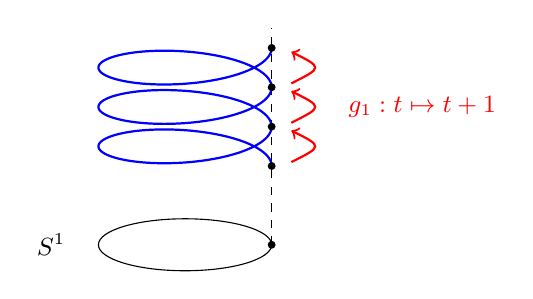
\begin{tikzpicture}[scale=1]
	\draw[thin, dashed] (1.1,-1.0) -- (1.1,1.75);
	\draw[thick, color=blue, samples=300, domain=0:1080, smooth, variable=\t]
		plot ({1.1*cos(\t)}, {0.33*sin(\t) + \t/720});
	\draw[thin] (0,-1.0) ellipse (1.1 and 0.33);
	\foreach \y in {0, 0.5, 1.0, 1.5} { \fill (1.1,\y) circle (0.05); }
	\fill (1.1,-1.0) circle (0.05);
	\draw[->, thick, color=red] (1.35,0.05) .. controls (1.75,0.25) .. (1.35,0.45);
	\draw[->, thick, color=red] (1.35,0.55) .. controls (1.75,0.75) .. (1.35,0.95);
	\draw[->, thick, color=red] (1.35,1.05) .. controls (1.75,1.25) .. (1.35,1.45);
	\node[color=red, right] at (1.95,0.75) {\small $g_1: t \mapsto t+1$};
	\node at (-1.7,-1.0) {\small $S^1$};
\end{tikzpicture}
\end{center}

\begin{example}
	For $p: \R \to S^1$, the deck group is $\{g_n : t \mapsto t + n \mid n \in \Z\} \cong \Z$. Indeed each $g_n$ satisfies $p \circ g_n = p$; conversely a deck transformation $g$ is a lift of $p$, determined by $g(0) \in p^{-1}(1) = \Z$, so $g = g_{g(0)}$. Note $G_D(p) \cong \Z \cong \pi_1(S^1)$.
\end{example}

\begin{example}
	For $p: S^n \to \RP^n$, the deck group is $\{\id, x \mapsto -x\} \cong \Z/2\Z$.
\end{example}

That the deck group of the helix covering agrees with $\pi_1(S^1)$ is no accident.

\begin{theorem} \label{thm:deck-pi1}
	Let $X$ be locally path connected and let $q: (\widetilde X, \tilde x_0) \to (X, x_0)$ be a universal cover. Then $G_D(q) \cong \pi_1(X, x_0)$.
\end{theorem}
\begin{proof}
	First, the evaluation map $G_D(q) \to q^{-1}(x_0)$, $g \mapsto g(\tilde x_0)$, is a bijection: given $\tilde x \in q^{-1}(x_0)$, Proposition \ref{prop:universal} (applied with $\hat X = \widetilde X$ and basepoint $\tilde x$) provides a unique covering transformation taking $\tilde x_0 \mapsto \tilde x$, and it is an isomorphism by the uniqueness corollary.

	Composing with the bijection $\varepsilon_q^{-1}: q^{-1}(x_0) \to \pi_1(X,x_0)$ of Proposition \ref{prop:eps-bijection}, we get a bijection $\Theta: \pi_1(X, x_0) \to G_D(q)$, characterised by $\Theta([\gamma])(\tilde x_0) = \tilde\gamma(1)$, where $\tilde\gamma$ is the lift of $\gamma$ at $\tilde x_0$.

	It remains to check that $\Theta$ is a homomorphism. Write $g = \Theta[\gamma]$ and $g' = \Theta[\gamma']$. Since $g$ is a deck transformation, $g \circ \tilde{\gamma'}$ is a lift of $\gamma'$ starting at $g(\tilde x_0) = \tilde\gamma(1)$, so
	$$
	\widetilde{\gamma\cdot\gamma'} = \tilde\gamma \cdot (g \circ \tilde{\gamma'}),
	$$
	whence
	$$
	\Theta[\gamma\cdot\gamma'](\tilde x_0) = \widetilde{\gamma\cdot\gamma'}(1) = g(\tilde{\gamma'}(1)) = g(g'(\tilde x_0)) = (g \circ g')(\tilde x_0).
	$$
	Both $\Theta[\gamma\cdot\gamma']$ and $g \circ g'$ are deck transformations sending $\tilde x_0$ to the same point, so they are equal.
\end{proof}

\subsection{The Galois Correspondence}

We can now describe \emph{all} the connected covers of a space in terms of the subgroup
structure of its fundamental group. Throughout, let $X$ be path connected and locally
path connected with universal cover $q: (\widetilde X, \tilde x_0) \to (X, x_0)$, and
identify $G = \pi_1(X, x_0)$ with the deck group $G_D(q)$ via Theorem \ref{thm:deck-pi1}.

Given a subgroup $H \leq G$, the group $H$ acts on $\widetilde X$ by deck transformations,
and we may form the quotient
$$
X_H = H \backslash \widetilde X,
$$
whose points are the orbits $H \cdot \tilde x$. Since deck transformations satisfy
$q \circ h = q$, the map $q$ descends to $p_H: X_H \to X$, $H\cdot\tilde x \mapsto q(\tilde x)$,
and we have a tower
\[\begin{tikzcd}
	{\widetilde X} \arrow[d, "{\pi_H}"'] & & 1 \arrow[d, no head] \\
	{X_H} \arrow[d, "{p_H}"'] & & H \arrow[d, no head] \\
	X & & G
\end{tikzcd}\]

\begin{proposition} \label{prop:quotient-cover}
	$\pi_H$ and $p_H$ are covering maps. If $H = G$ then $p_G$ is a covering isomorphism, so $X \cong G\backslash\widetilde X$.
\end{proposition}
\begin{proof}
	Let $x \in X$ and choose a path connected evenly covered neighbourhood $U$ of $x$, so $q^{-1}(U) = \bigsqcup_\alpha U_\alpha$. The deck group acts simply transitively on $q^{-1}(x)$, so the sheets are permuted simply transitively too, and we may index them as $q^{-1}(U) = \bigsqcup_{g \in G} g \cdot U_0$ for a fixed sheet $U_0$. Then the $H$-orbits of sheets are indexed by the cosets $gH$, giving
	$$
	p_H^{-1}(U) = \bigsqcup_{gH \in G/H} \pi_H\!\left(\textstyle\bigcup_{h\in H} gh\cdot U_0\right),
	$$
	and each piece maps homeomorphically onto $U$; similarly $\pi_H^{-1}$ of each piece is $\bigsqcup_{h \in H} gh \cdot U_0$. So $U$ is evenly covered by $p_H$ and each piece is evenly covered by $\pi_H$.

	If $H = G$ then $p_G$ is injective on fibres, hence bijective, hence a homeomorphism by Lemma \ref{lem:bijective-cover}.
\end{proof}

In particular a universal covering map is exactly the quotient by the action of
$\pi_1(X, x_0)$.

\begin{definition}
	A covering map $p: \hat X \to X$ is a \vocab{normal} (or regular) cover if $G_D(p)$ acts transitively on the fibre $p^{-1}(x_0)$.
\end{definition}

Now consider the two sets
\begin{align*}
	S(X, x_0) &= \{H \mid H \leq \pi_1(X,x_0)\}, \\
	C(X, x_0) &= \{(p, \hat X, \hat x_0) \mid p: (\hat X, \hat x_0) \to (X,x_0) \text{ a covering map, } \hat X \text{ path connected}\}/\!\sim,
\end{align*}
where $(p, \hat X, \hat x_0) \sim (p', \hat X', \hat x_0')$ if there is a covering
isomorphism between them matching the basepoints. Define
$$
\alpha: S(X,x_0) \to C(X,x_0), \quad \alpha(H) = (p_H, X_H, \pi_H(\tilde x_0)),
$$
$$
\beta: C(X,x_0) \to S(X,x_0), \quad \beta(p, \hat X, \hat x_0) = p_*(\pi_1(\hat X, \hat x_0)),
$$
noting that $\beta$ lands in subgroups by Corollary \ref{cor:p-injective}.

\begin{theorem}[Galois Correspondence] \label{thm:galois}
	$\alpha$ and $\beta$ are mutually inverse bijections.
\end{theorem}
\begin{proof}
	\emph{$\beta \circ \alpha = \id$.} Write $x_{0,H} = \pi_H(\tilde x_0)$. Given $[\gamma] \in H$ with lift $\tilde\gamma$ at $\tilde x_0$, the path $\pi_H \circ \tilde\gamma$ is a loop in $X_H$ at $x_{0,H}$, since $\tilde\gamma(1) = [\gamma]\cdot\tilde x_0$ lies in the same $H$-orbit as $\tilde x_0$. Moreover
	$$
	p_{H*}[\pi_H \circ \tilde\gamma] = [p_H \circ \pi_H \circ \tilde\gamma] = [q \circ \tilde\gamma] = [\gamma],
	$$
	so $H \subseteq \beta(\alpha(H))$. Conversely, if $[\gamma] = p_{H*}[\delta]$ for a loop $\delta$ in $X_H$, then the lift of $\gamma$ at $\tilde x_0$ ends at a point of $\pi_H^{-1}(x_{0,H}) = H\cdot\tilde x_0$, which says exactly that $[\gamma] \in H$.

	\emph{$\alpha \circ \beta = \id$.} Let $p: (\hat X, \hat x_0) \to (X, x_0)$ be a path connected cover and $H = p_*(\pi_1(\hat X, \hat x_0))$. By Proposition \ref{prop:universal} there is a covering transformation $\hat q: \widetilde X \to \hat X$ with $\hat q(\tilde x_0) = \hat x_0$, and it is surjective since $\hat X$ is path connected. We claim $\hat q$ is constant on $H$-orbits. Indeed let $h = [p\circ\delta] \in H$ for a loop $\delta$ in $\hat X$ at $\hat x_0$, and let $\tilde x \in \widetilde X$ with a path $\eta: \tilde x_0 \leadsto \tilde x$. Recall from the proof of Proposition \ref{prop:sc-lifting} that $\hat q(\tilde x) = \widehat{q\circ\eta}(1)$, the lift being taken at $\hat x_0$. Now $h \cdot \eta$ is a path from $h\cdot\tilde x_0$ to $h \cdot \tilde x$, so a path from $\tilde x_0$ to $h\cdot\tilde x$ is $\eta_h \cdot (h\circ\eta)$ where $\eta_h: \tilde x_0 \leadsto h \cdot \tilde x_0$ satisfies $q \circ \eta_h = p \circ \delta$. Hence
	$$
	\widehat{q \circ (\eta_h \cdot (h\circ \eta))} = \delta \cdot \widehat{q \circ \eta},
	$$
	and evaluating at $1$ gives $\hat q(h\cdot\tilde x) = \widehat{q\circ\eta}(1) = \hat q(\tilde x)$, as claimed.

	So $\hat q$ factors as $\hat q = p' \circ \pi_H$ for a map $p': X_H \to \hat X$, which is a covering transformation over $X$ taking $x_{0,H}$ to $\hat x_0$. It is surjective as $\hat q$ is, and injective because both $X_H$ and $\hat X$ have fibres over $x_0$ in bijection with $H\backslash G$ --- for $X_H$ by construction, for $\hat X$ by the first half of the proof. So $p'$ is a covering isomorphism, giving $\alpha(\beta(p,\hat X, \hat x_0)) = (p, \hat X, \hat x_0)$ in $C(X, x_0)$.
\end{proof}

The dictionary this sets up is worth spelling out.

\begin{remark} \label{rmk:galois-dictionary}
	Under the correspondence of Theorem \ref{thm:galois}:
	\begin{enumerate}
		\item the whole group $G$ corresponds to the trivial cover $(\id, X, x_0)$, and the trivial subgroup $1$ corresponds to the universal cover;
		\item the index $[G:H]$ equals the number of sheets $|p_H^{-1}(x_0)|$;
		\item changing the basepoint of a cover replaces $H$ by a conjugate: if $g = [\gamma]$ and $\hat\gamma$ is the lift of $\gamma$ to $X_H$ at $x_{0,H}$, then $(p_H, X_H, \hat\gamma(1))$ corresponds to $g^{-1}Hg$. So unbased covers correspond to conjugacy classes of subgroups;
		\item $p_H$ is a normal cover if and only if $H \normal G$, and in that case $G_D(p_H) \cong G/H$.
	\end{enumerate}
\end{remark}

\begin{example}
	Take $X = S^1$, so $G = \Z$. The subgroups are $n\Z$ for $n \geq 0$. The subgroup $0$ gives the universal cover $\R \to S^1$, and $n\Z$ for $n \geq 1$ gives the $n$-sheeted cover $S^1 \to S^1$, $z \mapsto z^n$: indeed $p_{n*}(\pi_1(S^1)) = n\Z$, since $p_n$ takes a generating loop to a loop of winding number $n$. As $\Z$ is abelian, every cover of $S^1$ is normal, with deck group $\Z/n\Z$. This is the complete list of connected covers of the circle.
\end{example}

\begin{example}
	The two-sheeted cover $S^n \to \RP^n$ is universal for $n \geq 2$, since we will show in the next section that $S^n$ is simply connected for $n \geq 2$. Hence
	$$
	\pi_1(\RP^n) \cong G_D(p) \cong \Z/2\Z \qquad (n \geq 2).
	$$
\end{example}

\section{The Seifert--van Kampen Theorem}

Covering space theory computed $\pi_1(S^1)$, and with it $\pi_1$ of anything built out of
circles by taking products or quotients by nice group actions. That is a rather short
list. The Seifert--van Kampen theorem is the general computational tool: it tells us how
to assemble $\pi_1(X)$ from $\pi_1$ of the pieces of an open cover of $X$ by two sets.
Before we can state it we need the group theory it takes values in.

\subsection{Wedges and Free Groups}

\begin{definition}[Wedge]
	Let $(X_i, x_i)$ for $1 \leq i \leq n$ be based spaces. Their \vocab{wedge} is
	$$
	\bigvee_{i=1}^n (X_i, x_i) = \left(\coprod_{i=1}^n X_i\right)\Big/\!\sim,
	$$
	where $\sim$ is generated by $x_i \sim x_j$ for all $i, j$. That is, we glue the spaces together at their basepoints.
\end{definition}

The example we care about is the \vocab{figure-eight} $S^1 \vee S^1$, and more generally
the wedge of $n$ circles.

\begin{center}
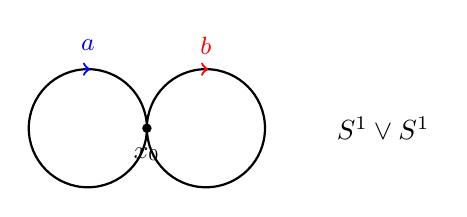
\begin{tikzpicture}[scale=1]
	\draw[thick] (-0.75,0) circle (0.75);
	\draw[thick] (0.75,0) circle (0.75);
	\fill (0,0) circle (0.06);
	\node[below] at (0,-0.12) {\small $x_0$};
	\draw[->, thick, color=blue] (-0.78,0.75) -- (-0.72,0.75);
	\node[color=blue] at (-0.75,1.05) {\small $a$};
	\draw[->, thick, color=red] (0.72,0.75) -- (0.78,0.75);
	\node[color=red] at (0.75,1.05) {\small $b$};
	\node at (3.0,0) {$S^1 \vee S^1$};
\end{tikzpicture}
\end{center}

Write $\iota_1, \iota_2: (S^1, 1) \to (S^1 \vee S^1, x_0)$ for the two inclusions, and set
$a = \iota_{1*}(1)$, $b = \iota_{2*}(1)$ in $\pi_1(S^1 \vee S^1, x_0)$. What group do
$a$ and $b$ generate? We can answer this with covering spaces.

Let $T_\infty(4)$ be the infinite $4$-valent tree: the connected graph in which every
vertex has exactly four neighbours and there are no cycles, topologised as the union of
its finite subtrees $T_n(4)$ (so $U$ is open exactly when each $U \cap T_n(4)$ is).

\begin{center}
\begin{tikzpicture}[scale=1]
	\def\lena{1.15}
	\def\lenb{0.65}
	\def\lenc{0.22}
	% centre
	\fill (0,0) circle (0.055);
	\foreach \a in {0,90,180,270} {
		\draw[thick, color=blue] (0,0) -- (\a:\lena);
	}
	\foreach \a in {0,90,180,270} {
		\fill (\a:\lena) circle (0.045);
		\foreach \b in {-90,0,90} {
			\draw[thick, color=blue] (\a:\lena) -- ++(\a+\b:\lenb);
			\fill ($(\a:\lena)+(\a+\b:\lenb)$) circle (0.035);
			\foreach \c in {-90,0,90} {
				\draw[thin, color=blue] ($(\a:\lena)+(\a+\b:\lenb)$) -- ++(\a+\b+\c:\lenc);
			}
		}
	}
	\node at (0.22,-0.25) {\small $\tilde x_0$};
\end{tikzpicture}
\end{center}

\begin{proposition} \label{prop:tree-cover}
	There is a covering map $q: T_\infty(4) \to S^1 \vee S^1$, and $T_\infty(4)$ is simply connected. So $T_\infty(4)$ is the universal cover of the figure-eight.
\end{proposition}
\begin{proof}
	Colour the four edges at each vertex with the labels $a, a^{-1}, b, b^{-1}$, one each, in such a way that the $a$-edge out of $v$ is the $a^{-1}$-edge out of its other endpoint, and similarly for $b$. Now map each $a$-labelled edge homeomorphically onto the first circle, respecting orientation, and each $b$-labelled edge onto the second, sending all vertices to $x_0$. A point in the interior of an edge has a neighbourhood inside that edge which is evenly covered, and a small star-shaped neighbourhood of $x_0$ (a little arc of each circle either side) is evenly covered by the corresponding small stars around each vertex. So $q$ is a covering map.

	For simple connectedness: $I$ is compact, so the image of any path lies in some finite subtree $T_n(4)$. A finite tree is contractible --- collapse the leaves one at a time --- and hence simply connected, so any loop in $T_\infty(4)$ is null-homotopic within $T_n(4)$, and so within $T_\infty(4)$.
\end{proof}

\begin{corollary} \label{cor:fig8-nonabelian}
	$\pi_1(S^1 \vee S^1, x_0)$ is not abelian.
\end{corollary}
\begin{proof}
	By Proposition \ref{prop:eps-bijection}, $\varepsilon_q: \pi_1(S^1\vee S^1, x_0) \to q^{-1}(x_0)$ is a bijection onto the vertex set of the tree. Lifting the loop $a \cdot b$ at $\tilde x_0$, we travel along the $a$-edge and then a $b$-edge; lifting $b \cdot a$, we travel along the $b$-edge and then an $a$-edge. These end at different vertices, so $ab \neq ba$.
\end{proof}

The bijection in that proof does more: it identifies $\pi_1(S^1 \vee S^1)$ completely. A
vertex $\tilde x$ of the tree is joined to $\tilde x_0$ by a unique shortest path, and
recording the labels of the edges traversed gives an `address' for $\tilde x$, namely a
word $w = \ell_1\ell_2\cdots\ell_r$ in the letters $a^{\pm1}, b^{\pm1}$ containing no
substring $aa^{-1}, a^{-1}a, bb^{-1}, b^{-1}b$ --- a \vocab{reduced word}. Conversely
every reduced word is the address of exactly one vertex. Under $\varepsilon_q$,
multiplication in $\pi_1$ corresponds to concatenating words and then cancelling.
This is precisely the free group.

\begin{definition}[Free Group]
	A \vocab{free group} on a set $S$ is a group $F_S$ together with a function $S \to F_S$ such that for any group $G$ and any function $\varphi: S \to G$ there is a unique homomorphism $\Phi: F_S \to G$ restricting to $\varphi$ on $S$.
	\[\begin{tikzcd}
		& {F_S} \arrow[d, "\Phi", dashed] \\
		S \arrow[ru] \arrow[r, "\varphi"'] & G
	\end{tikzcd}\]
\end{definition}

\begin{lemma}
	If $F_S$ and $F_S'$ are both free on $S$ then $F_S \cong F_S'$; more generally a bijection $S \to T$ induces an isomorphism $F_S \to F_T$. So the isomorphism type of $F_S$ depends only on $|S|$, and we write $F_n$ for the free group on $n$ generators.
\end{lemma}
\begin{proof}
	Let $\varphi: S \to T$ be a bijection with inverse $\psi$, and let $\Phi: F_S \to F_T$ and $\Psi: F_T \to F_S$ be the induced homomorphisms. Then $\Psi \circ \Phi: F_S \to F_S$ restricts to the identity on $S$; but so does $\id_{F_S}$, and the universal property says there is only one such homomorphism. So $\Psi \circ \Phi = \id$, and by symmetry $\Phi \circ \Psi = \id$.
\end{proof}

\begin{theorem} \label{thm:pi1-wedge-circles}
	$\pi_1\!\left(\bigvee_{i=1}^n S^1\right) \cong F_n$, free on the classes $a_1, \dots, a_n$ of the $n$ circles.
\end{theorem}
\begin{proof}
	Exactly as above, the universal cover of $\bigvee_{i=1}^n S^1$ is the infinite $2n$-valent tree $T_\infty(2n)$, and $\varepsilon_q$ identifies $\pi_1$ with the set of reduced words in $a_1^{\pm1},\dots,a_n^{\pm1}$, with multiplication given by concatenate-and-cancel. It remains to check the universal property. Given $\varphi: \{a_1,\dots,a_n\} \to G$, extend it to inverses by $\varphi(a_i^{-1}) = \varphi(a_i)^{-1}$ and define
	$$
	\Phi(\ell_1\cdots\ell_r) = \varphi(\ell_1)\cdots\varphi(\ell_r).
	$$
	This is a homomorphism, since concatenating two reduced words and cancelling a substring $\ell\ell^{-1}$ has no effect on the right hand side. It is the unique homomorphism restricting to $\varphi$, since the $a_i$ generate.
\end{proof}

We will express our answers as presentations, so let us fix notation. For $S \subseteq G$
we write $\genby{S}$ for the smallest subgroup containing $S$ and $\ngenby{S}$ for the
smallest \emph{normal} subgroup containing $S$ (the intersection of all such, which is a
normal subgroup).

\begin{definition}[Presentation]
	Given a set $S$ and $R \subseteq F_S$, we write $\genby{S \mid R} = F_S / \ngenby{R}$. If $G \cong \genby{S\mid R}$ we call $\genby{S\mid R}$ a \vocab{presentation} of $G$, with \vocab{generators} $S$ and \vocab{relations} $R$.
\end{definition}

Every group has a presentation: take $S = G$ and $R = \ker(\Phi_G: F_G \to G)$. Usually we
want much smaller ones.

\begin{example}
	$\genby{a \mid \varnothing} \cong \Z$, $\genby{a \mid a^n} \cong \Z/n\Z$, $\genby{a, b \mid \varnothing} \cong F_2$, and $\genby{a,b \mid aba^{-1}b^{-1}} \cong \Z^2$. Note that $\genby{a,b\mid ab^{-3}} \cong \Z$, since $a$ can be eliminated.
\end{example}

The last example is an instance of a general and very useful move.

\begin{proposition} \label{prop:tietze}
	Let $\genby{S \mid R}$ be a presentation, let $a \notin S$ and let $w \in F_S$. Then
	$$
	\genby{S \mid R} \cong \genby{S \cup \{a\} \mid R \cup \{aw^{-1}\}}.
	$$
\end{proposition}
\begin{proof}
	Define $\varphi$ from left to right by $s \mapsto s$, and $\psi$ from right to left by $s \mapsto s$ and $a \mapsto w$; both are well-defined as they respect the relations. They are mutually inverse.
\end{proof}

We will also freely use that a relation may be replaced by a conjugate of itself, or
multiplied by another relation, without changing the group.

\begin{remark}
	One should not get too optimistic about presentations. It is a theorem of Novikov and Boone that there is no algorithm which, given a finite presentation, decides whether the group it presents is trivial. So `compute $\pi_1$' can only ever mean `write down a presentation'.
\end{remark}

\subsection{Amalgamated Free Products}

\begin{definition}[Amalgamated Free Product]
	Let $\iota_1: H \to G_1$ and $\iota_2: H \to G_2$ be group homomorphisms. A group $G$ is an \vocab{amalgamated free product} of $G_1$ and $G_2$ along $H$ if
	\begin{enumerate}
		\item there are homomorphisms $\varphi_i: G_i \to G$ with $\varphi_1 \circ \iota_1 = \varphi_2 \circ \iota_2$; and
		\item this is universal: for any group $\bar G$ with homomorphisms $j_i: G_i \to \bar G$ satisfying $j_1 \circ\iota_1 = j_2\circ\iota_2$, there is a unique $\psi: G \to \bar G$ with $\psi \circ \varphi_i = j_i$.
	\end{enumerate}
	\[\begin{tikzcd}
		& {G_1} \arrow[rd, "{\varphi_1}"'] \arrow[rrd, "{j_1}", bend left] & & \\
		H \arrow[ru, "{\iota_1}"] \arrow[rd, "{\iota_2}"'] & & G \arrow[r, "\psi", dashed] & {\bar G} \\
		& {G_2} \arrow[ru, "{\varphi_2}"] \arrow[rru, "{j_2}"', bend right] & &
	\end{tikzcd}\]
	We write $G = G_1 *_H G_2$.
\end{definition}

Categorically this is a pushout; concretely it is `$G_1$ and $G_2$ glued along $H$, with
no relations imposed beyond those forced'. As with all universal properties, uniqueness
is automatic.

\begin{proposition}
	If $G$ and $G'$ are both amalgamated free products of $G_1, G_2$ along $H$, then $G \cong G'$.
\end{proposition}
\begin{proof}
	Universality gives $\alpha: G \to G'$ and $\beta: G' \to G$ compatible with the $\varphi_i$. Then $\beta\circ\alpha: G \to G$ is compatible with the $\varphi_i$, as is $\id_G$, so uniqueness forces $\beta\circ\alpha = \id_G$; likewise $\alpha\circ\beta = \id_{G'}$.
\end{proof}

\begin{proposition} \label{prop:afp-exists}
	Amalgamated free products exist. Explicitly, if $G_i = \genby{S_i \mid R_i}$ and $H = \genby{T \mid W}$, then
	$$
	G_1 *_H G_2 = \left\langle S_1 \sqcup S_2 \;\middle|\; R_1 \cup R_2 \cup \{\iota_1(t)\iota_2(t)^{-1} \mid t \in T\}\right\rangle,
	$$
	where $\iota_i(t)$ is read as a word in $S_i$.
\end{proposition}
\begin{proof}
	Call the right hand side $G$, and let $\varphi_i: G_i \to G$ send $s \in S_i$ to $s$; this is well-defined since the relations $R_i$ hold in $G$. The added relations say exactly that $\varphi_1 \circ\iota_1$ and $\varphi_2\circ\iota_2$ agree on the generators $T$ of $H$, hence agree.

	Given $j_1, j_2$ into $\bar G$ as in the definition, define $\psi$ on generators by $\psi(s) = j_i(s)$ for $s \in S_i$. The relations in $R_i$ are satisfied because $j_i$ is a homomorphism, and the relation $\iota_1(t)\iota_2(t)^{-1}$ is satisfied because $j_1\iota_1(t) = j_2\iota_2(t)$. So $\psi$ is a well-defined homomorphism, and it is the unique one with $\psi\circ\varphi_i = j_i$ since the $S_i$ generate $G$.
\end{proof}

\begin{example}
	If $H = 1$ we write $G_1 * G_2$, the \vocab{free product}. For instance $F_m * F_n \cong F_{m+n}$, and $\Z * \Z \cong F_2$.
\end{example}

\subsection{The Theorem}

We first prove the `easy half', which is already useful on its own.

\begin{theorem} \label{thm:vk-generation}
	Let $X = U_1 \cup U_2$ with $U_1, U_2$ open, and suppose $U_1 \cap U_2$ is path connected with $x_0 \in U_1 \cap U_2$. Let $j_i: U_i \hookrightarrow X$ be the inclusions. Then $\pi_1(X, x_0)$ is generated by
	$$
	j_{1*}(\pi_1(U_1,x_0)) \cup j_{2*}(\pi_1(U_2,x_0)).
	$$
\end{theorem}
\begin{proof}
	Let $\gamma$ be a loop at $x_0$. Then $\{\gamma^{-1}(U_1), \gamma^{-1}(U_2)\}$ is an open cover of $I$, so by the Lebesgue covering lemma there is $n$ such that each $[\frac{j}{n},\frac{j+1}{n}]$ maps into $U_1$ or into $U_2$; label each subinterval accordingly, choosing arbitrarily if both work. Amalgamating adjacent subintervals with the same label, we get $0 = t_0 < t_1 < \dots < t_k = 1$ and paths $\gamma_i = \gamma|_{[t_{i-1},t_i]}$, each contained in a single $U_{c(i)}$, with consecutive labels different. In particular each $\gamma(t_i)$ for $0 < i < k$ lies in $U_1 \cap U_2$.

	Since $U_1 \cap U_2$ is path connected, choose paths $\eta_i: \gamma(t_i) \leadsto x_0$ inside $U_1 \cap U_2$ for $1 \leq i \leq k-1$. Inserting $\eta_i \cdot \eta_i^{-1}$ at each break point,
	$$
	\gamma \simeq (\gamma_1\cdot\eta_1)\cdot(\eta_1^{-1}\cdot\gamma_2\cdot\eta_2)\cdots(\eta_{k-1}^{-1}\cdot\gamma_k) = \delta_1 \cdot \delta_2 \cdots \delta_k,
	$$
	where each $\delta_i$ is a loop at $x_0$ lying entirely inside $U_{c(i)}$. Hence $[\gamma] = [\delta_1]\cdots[\delta_k]$ is a product of elements of $j_{1*}(\pi_1(U_1,x_0)) \cup j_{2*}(\pi_1(U_2,x_0))$.
\end{proof}

\begin{center}
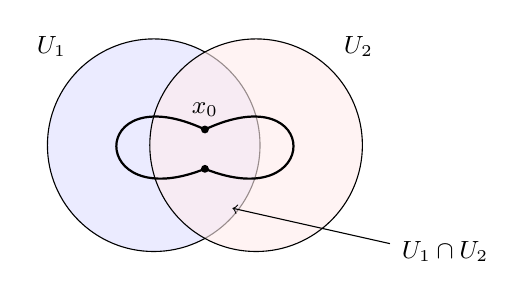
\begin{tikzpicture}[scale=1]
	\draw[thin, fill=blue!8] (-0.65,0) circle (1.35);
	\draw[thin, fill=red!8, fill opacity=0.6] (0.65,0) circle (1.35);
	\node at (-1.95,1.25) {\small $U_1$};
	\node at (1.95,1.25) {\small $U_2$};
	\draw[thin, ->] (2.35,-1.25) -- (0.35,-0.8);
	\node at (3.05,-1.35) {\small $U_1 \cap U_2$};
	\fill (0,0.2) circle (0.05);
	\node at (0.0,0.45) {\small $x_0$};
	% loop crossing
	\draw[thick] (0,0.2) .. controls (-1.5,0.9) and (-1.5,-0.9) .. (0,-0.3);
	\draw[thick] (0,-0.3) .. controls (1.5,-0.9) and (1.5,0.9) .. (0,0.2);
	\fill (0,-0.3) circle (0.05);
\end{tikzpicture}
\end{center}

\begin{corollary} \label{cor:sphere-sc}
	If $X = U_1 \cup U_2$ with $U_1, U_2$ open and simply connected and $U_1 \cap U_2$ path connected and non-empty, then $X$ is simply connected.
\end{corollary}
\begin{proof}
	$\pi_1(X, x_0)$ is generated by the trivial group.
\end{proof}

\begin{example} \label{ex:sn-sc}
	$S^n$ is simply connected for $n \geq 2$. Take $U^{\pm} = S^n \setminus \{\mp e_1\}$, the sphere with one point removed. Both are homeomorphic to $\R^n$ by stereographic projection, hence simply connected, and
	$$
	U^+ \cap U^- \cong \R^n \setminus\{0\} \simeq S^{n-1},
	$$
	which is path connected precisely when $n \geq 2$.
\end{example}

Note how badly this fails for $n = 1$: there $U^+ \cap U^-$ has two components, and
indeed $\pi_1(S^1) = \Z$. The full theorem tells us exactly how the failure of $\pi_1(X)$
to be generated freely is controlled by $\pi_1(U_1 \cap U_2)$.

\begin{theorem}[Seifert--van Kampen] \label{thm:vk}
	Let $X = U_1 \cup U_2$ with $U_1, U_2$ open and $U_1 \cap U_2$ path connected containing $x_0$; suppose also that $U_1, U_2$ are path connected. Write $G_i = \pi_1(U_i, x_0)$ and $H = \pi_1(U_1\cap U_2, x_0)$, with $\iota_{i*}: H \to G_i$ induced by the inclusions. Then
	$$
	\pi_1(X, x_0) \cong G_1 *_H G_2 .
	$$
\end{theorem}
\begin{proof}
	The square of inclusions
	\[\begin{tikzcd}
		& {U_1} \arrow[rd, "{j_1}"] & & & & {G_1} \arrow[rd, "{j_{1*}}"] & \\
		{U_1\cap U_2} \arrow[ru, "{\iota_1}"] \arrow[rd, "{\iota_2}"'] & & X & & H \arrow[ru, "{\iota_{1*}}"] \arrow[rd, "{\iota_{2*}}"'] & & {\pi_1(X,x_0)} \\
		& {U_2} \arrow[ru, "{j_2}"'] & & & & {G_2} \arrow[ru, "{j_{2*}}"'] &
	\end{tikzcd}\]
	commutes, so applying $\pi_1$ gives a commuting square of groups. By the universal property of the amalgamated free product there is a unique homomorphism
	$$
	\psi: G_1 *_H G_2 \to \pi_1(X, x_0)
	$$
	with $\psi \circ \varphi_i = j_{i*}$. It is surjective by Theorem \ref{thm:vk-generation}, since its image contains both $j_{i*}(G_i)$. The work is in showing that it is injective.

	So suppose $g \in G_1 *_H G_2$ has $\psi(g) = 1$. Write $g = \varphi_{c(1)}(g_1)\cdots\varphi_{c(k)}(g_k)$ as a product of images of elements $g_i \in G_{c(i)}$, and represent each $g_i$ by a loop $\delta_i$ in $U_{c(i)}$ based at $x_0$. Then $\gamma = \delta_1 \cdots \delta_k$ is a loop in $X$ with $[\gamma] = 1$, so there is a homotopy $F: I \times I \to X$ with $F(s, 0) = \gamma(s)$, $F(s,1) = x_0$ and $F(0,t) = F(1,t) = x_0$.

	Apply the Lebesgue covering lemma to the open cover $\{F^{-1}(U_1), F^{-1}(U_2)\}$ of $I^2$ to get $n$ such that each small square $A = [\frac{i}{n},\frac{i+1}{n}]\times[\frac{j}{n},\frac{j+1}{n}]$ has $F(A)$ inside some $U_{c(A)}$; refining $n$ further we may assume the break points of $\gamma$ occur at multiples of $1/n$. For each vertex $v$ of the grid choose a path $\eta_v$ from $x_0$ to $F(v)$, lying in $U_1 \cap U_2$ if $F(v) \in U_1\cap U_2$, and in $U_{c}$ if $F(v)$ only lies in $U_{c}$; take $\eta_v$ constant when $F(v) = x_0$. For each edge $e$ of the grid with endpoints $v, w$, we get a loop
	$$
	\lambda_e = \eta_v \cdot (F\circ e)\cdot \eta_w^{-1}
	$$
	based at $x_0$, lying in whichever $U_c$ contains the squares adjacent to $e$; if both indices are available, $\lambda_e$ lies in $U_1 \cap U_2$ and so determines an element of $H$, whose images in $G_1$ and $G_2$ are identified in $G_1 *_H G_2$. In every case, then, $\lambda_e$ determines a well-defined element $[\lambda_e] \in G_1 *_H G_2$.

	Now let $\rho_j \in G_1*_HG_2$ be the product of the $[\lambda_e]$ along the horizontal grid line at height $j/n$, read left to right. Two facts finish the proof.
	\begin{enumerate}
		\item $\rho_0 = g$ and $\rho_n = 1$. The bottom row is $\gamma$, cut at the break points, and since the $\eta_v$ for $v$ on the bottom row are constant we get exactly $\varphi_{c(1)}(g_1)\cdots\varphi_{c(k)}(g_k) = g$. The top row is constant at $x_0$, so all its edge loops are trivial.
		\item $\rho_j = \rho_{j+1}$ for each $j$. Consider a single square $A$ between the two rows, with $F(A) \subseteq U_{c(A)}$. Its four edge loops $\lambda_e$ all lie in $U_{c(A)}$, and $F|_A$ shows that the composite loop around $\partial A$ is null-homotopic \emph{in $U_{c(A)}$}, because $A$ is convex. Hence in $G_{c(A)}$, and therefore in $G_1 *_H G_2$, the product of the bottom and right edge classes equals the product of the left and top edge classes. Multiplying these relations across the row, and cancelling the interior vertical edges in pairs, converts $\rho_j$ into $\rho_{j+1}$.
	\end{enumerate}
	Therefore $g = \rho_0 = \rho_n = 1$, and $\psi$ is injective.
\end{proof}

\begin{center}
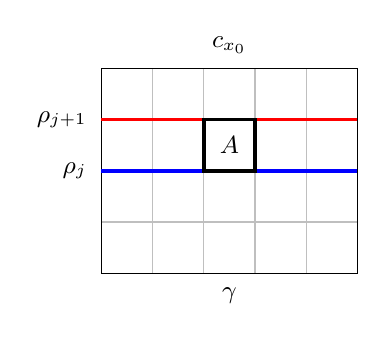
\begin{tikzpicture}[scale=0.65]
	\draw[color=lightgray, thin] (0,0) grid (5,4);
	\draw[thin] (0,0) rectangle (5,4);
	\draw[very thick, color=blue] (0,2) -- (5,2);
	\draw[very thick, color=red] (0,3) -- (5,3);
	\node[left] at (-0.1,2) {\small $\rho_j$};
	\node[left] at (-0.1,3) {\small $\rho_{j+1}$};
	\draw[very thick] (2,2) rectangle (3,3);
	\node at (2.5,2.5) {\small $A$};
	\node[below] at (2.5,-0.1) {\small $\gamma$};
	\node[above] at (2.5,4.1) {\small $c_{x_0}$};
\end{tikzpicture}
\end{center}

\subsection{Applications}

The most common way to apply the theorem is to a space built by gluing a disc onto
another space along its boundary circle.

\begin{definition}
	Let $f: S^1 \to X$ be a map. The space obtained by \vocab{attaching a $2$-cell} along $f$ is
	$$
	X \cup_f D^2 = (X \sqcup D^2)/\!\sim, \qquad z \sim f(z) \text{ for } z \in S^1 .
	$$
\end{definition}

\begin{proposition} \label{prop:attach-cell}
	Let $X$ be path connected with $x_0 = f(1)$, and suppose $\pi_1(X,x_0) = \genby{S \mid R}$. Then
	$$
	\pi_1(X\cup_f D^2, x_0) \cong \pi_1(X, x_0)\big/\ngenby{f_*(1)} = \genby{S \mid R \cup \{w_f\}},
	$$
	where $w_f$ is any word representing the class $f_*(1) \in \pi_1(X,x_0)$ of the attaching loop.
\end{proposition}
\begin{proof}
	Let $\pi: X \sqcup D^2 \to X\cup_f D^2$ be the quotient map and set
	$$
	U_1 = \pi(X \sqcup (D^2\setminus\{0\})), \qquad U_2 = \pi((D^2)^\circ).
	$$
	These are open, $U_1 \cup U_2 = X \cup_f D^2$, and $U_1 \cap U_2 = \pi((D^2)^\circ \setminus \{0\})$ is path connected. Now $D^2 \setminus\{0\}$ strong deformation retracts onto $S^1$, so $U_1$ strong deformation retracts onto $X$, giving $\pi_1(U_1) \cong \pi_1(X, x_0)$. Also $\pi_1(U_2) = 1$ as $(D^2)^\circ$ is convex, and $U_1 \cap U_2 \simeq S^1$, so $H = \pi_1(U_1\cap U_2) \cong \Z = \genby{t}$, generated by a small loop around the puncture. Under $\iota_{1*}$ this maps to the class of the attaching loop $f_*(1)$, and under $\iota_{2*}$ to $1$.

	(Strictly, the basepoint must be moved into $U_1 \cap U_2$; we conjugate by a path to $x_0$, which is harmless.) By Theorem \ref{thm:vk} and Proposition \ref{prop:afp-exists},
	$$
	\pi_1(X\cup_f D^2) \cong \genby{S \mid R} *_{\genby{t}} 1 = \genby{S, t \mid R \cup \{t^{-1}w_f, \, t\}} \cong \genby{S \mid R \cup \{w_f\}}. \qedhere
	$$
\end{proof}

In words: attaching a disc kills the class of the loop you attach it along, and nothing
else. We can now compute the fundamental groups of all the closed surfaces, because every
closed surface is a polygon with its edges identified in pairs --- which is to say, a
wedge of circles with a single disc attached.

\begin{example}[The Torus] \label{ex:torus-vk}
	Take the square $I^2$ and identify its edges according to the word $aba^{-1}b^{-1}$, meaning that we glue the left edge to the right edge and the bottom to the top, both without a flip. The result is $T^2$. Its $1$-skeleton --- the image of $\partial I^2$ --- is $S^1 \vee S^1$, since all four corners are identified to a single point, and the interior of the square is a $2$-cell attached along the loop $a\cdot b\cdot a^{-1}\cdot b^{-1}$. So by Theorem \ref{thm:pi1-wedge-circles} and Proposition \ref{prop:attach-cell},
	$$
	\pi_1(T^2) \cong \genby{a, b \mid aba^{-1}b^{-1}} \cong \Z^2,
	$$
	agreeing with the computation in Example \ref{ex:pi1-torus}.
\end{example}

\begin{example}[The Klein Bottle]
	Identify the edges of $I^2$ according to $abab^{-1}$: the left and right edges are glued as before, but the bottom and top are glued with a flip. The result is the Klein bottle $K$, and
	$$
	\pi_1(K) \cong \genby{a,b \mid abab^{-1}}.
	$$
	The relation rearranges to $bab^{-1} = a^{-1}$, so this group is the semidirect product $\Z \rtimes \Z$ in which the second factor acts on the first by inversion. In particular it is not abelian. Its abelianisation is $\Z/2\Z \times \Z$, whereas $\pi_1(T^2)^{\mathrm{ab}} = \Z^2$ is torsion-free, so $K \not\simeq T^2$ and in particular the Klein bottle is not homeomorphic to the torus.
\end{example}

\begin{center}
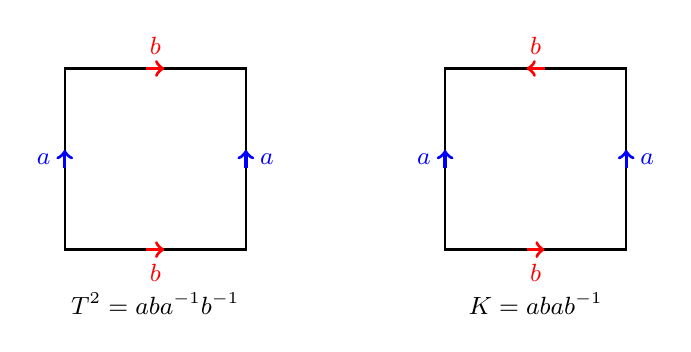
\begin{tikzpicture}[scale=1.15]
	% torus square
	\draw[thick] (0,0) rectangle (2,2);
	\draw[->, very thick, color=blue] (0,0.9) -- (0,1.1);
	\draw[->, very thick, color=blue] (2,0.9) -- (2,1.1);
	\draw[->, very thick, color=red] (0.9,0) -- (1.1,0);
	\draw[->, very thick, color=red] (0.9,2) -- (1.1,2);
	\node[color=blue, left] at (-0.05,1) {\small $a$};
	\node[color=blue, right] at (2.05,1) {\small $a$};
	\node[color=red, below] at (1,-0.05) {\small $b$};
	\node[color=red, above] at (1,2.05) {\small $b$};
	\node at (1,-0.6) {\small $T^2 = aba^{-1}b^{-1}$};
	% klein square
	\begin{scope}[xshift=4.2cm]
	\draw[thick] (0,0) rectangle (2,2);
	\draw[->, very thick, color=blue] (0,0.9) -- (0,1.1);
	\draw[->, very thick, color=blue] (2,0.9) -- (2,1.1);
	\draw[->, very thick, color=red] (0.9,0) -- (1.1,0);
	\draw[->, very thick, color=red] (1.1,2) -- (0.9,2);
	\node[color=blue, left] at (-0.05,1) {\small $a$};
	\node[color=blue, right] at (2.05,1) {\small $a$};
	\node[color=red, below] at (1,-0.05) {\small $b$};
	\node[color=red, above] at (1,2.05) {\small $b$};
	\node at (1,-0.6) {\small $K = abab^{-1}$};
	\end{scope}
\end{tikzpicture}
\end{center}

\begin{example}[The Projective Plane]
	Identifying the edges of $I^2$ by $abab$, equivalently identifying antipodal points on the boundary of a disc, gives $\RP^2$. The $1$-skeleton is a single circle $\genby{a}$ and the disc is attached along $a^2$, so
	$$
	\pi_1(\RP^2) \cong \genby{a \mid a^2} \cong \Z/2\Z,
	$$
	as we already knew from the covering $S^2 \to \RP^2$.
\end{example}

\begin{example}[Surfaces of Genus $g$] \label{ex:genus-g}
	Let $\Sigma_g$ be the closed orientable surface of genus $g$, obtained from a $4g$-gon by identifying its edges according to the word
	$$
	a_1b_1a_1^{-1}b_1^{-1}a_2b_2a_2^{-1}b_2^{-1}\cdots a_gb_ga_g^{-1}b_g^{-1}.
	$$
	All $4g$ vertices are identified to a point, so the $1$-skeleton is $\bigvee_{i=1}^{2g}S^1$, and hence
	$$
	\pi_1(\Sigma_g) \cong \left\langle a_1,b_1,\dots,a_g,b_g \;\middle|\; \prod_{i=1}^g a_ib_ia_i^{-1}b_i^{-1}\right\rangle.
	$$
	Abelianising gives $\Z^{2g}$, so the $\Sigma_g$ are pairwise non-homotopy-equivalent.
\end{example}

\begin{center}
\begin{tikzpicture}[scale=1.5]
	\draw[thick] (22.5:1) \foreach \i in {1,...,8} { -- (22.5+45*\i:1) };
	\foreach \i/\lab/\dir in {0/{a_1}/1, 1/{b_1}/1, 2/{a_1}/-1, 3/{b_1}/-1, 4/{a_2}/1, 5/{b_2}/1, 6/{a_2}/-1, 7/{b_2}/-1} {
		\node at ({22.5+45*\i+22.5}:1.2) {\small $\lab$};
	}
	\foreach \i in {0,...,7} {
		\coordinate (P) at ({22.5+45*\i}:1);
		\coordinate (Q) at ({22.5+45*(\i+1)}:1);
		\fill (P) circle (0.025);
	}
	\draw[->, very thick, color=blue] ($(22.5:1)!0.45!(67.5:1)$) -- ($(22.5:1)!0.55!(67.5:1)$);
	\draw[->, very thick, color=red] ($(67.5:1)!0.45!(112.5:1)$) -- ($(67.5:1)!0.55!(112.5:1)$);
	\draw[->, very thick, color=blue] ($(157.5:1)!0.45!(112.5:1)$) -- ($(157.5:1)!0.55!(112.5:1)$);
	\draw[->, very thick, color=red] ($(202.5:1)!0.45!(157.5:1)$) -- ($(202.5:1)!0.55!(157.5:1)$);
	\draw[->, very thick, color=blue] ($(202.5:1)!0.45!(247.5:1)$) -- ($(202.5:1)!0.55!(247.5:1)$);
	\draw[->, very thick, color=red] ($(247.5:1)!0.45!(292.5:1)$) -- ($(247.5:1)!0.55!(292.5:1)$);
	\draw[->, very thick, color=blue] ($(337.5:1)!0.45!(292.5:1)$) -- ($(337.5:1)!0.55!(292.5:1)$);
	\draw[->, very thick, color=red] ($(22.5:1)!0.45!(337.5:1)$) -- ($(22.5:1)!0.55!(337.5:1)$);
	\node at (0,-1.75) {\small $\Sigma_2$};
\end{tikzpicture}
\end{center}

Alternatively, we can cut a genus $2$ surface along a circle into two one-holed tori,
which gives $\pi_1(\Sigma_2) \cong \genby{a_1,b_1}*_\Z\genby{a_2,b_2}$, with the
amalgamation identifying the two commutators.

Finally, here is a taste of where these techniques lead. A \vocab{knot} is an embedding
$S^1 \hookrightarrow S^3$, and the basic problem is to tell knots apart. Since all knots
are homeomorphic to $S^1$ as spaces, we must look instead at the complement.

\begin{example}[Knot Complements]
	Let $U \subseteq S^3$ be the \vocab{unknot}, a round circle. Then $S^3 \setminus U$ deformation retracts onto a circle (spin around the axis of the unknot), so
	$$
	\pi_1(S^3\setminus U) \cong \Z.
	$$
	Now let $T$ be the \vocab{trefoil}. Cutting $S^3$ into the two solid tori on either side of the standard torus, on which $T$ can be drawn as a curve of slope $3/2$, and applying Seifert--van Kampen gives
	$$
	\pi_1(S^3 \setminus T) \cong \genby{x, y \mid x^2 = y^3}.
	$$
	This group surjects onto $S_3$: send $x \mapsto (1\,2)$ and $y \mapsto (1\,2\,3)$, and check $x^2 = e = y^3$. So $\pi_1(S^3\setminus T)$ is non-abelian, and in particular not $\Z$. Hence the trefoil is genuinely knotted.
\end{example}

\begin{center}
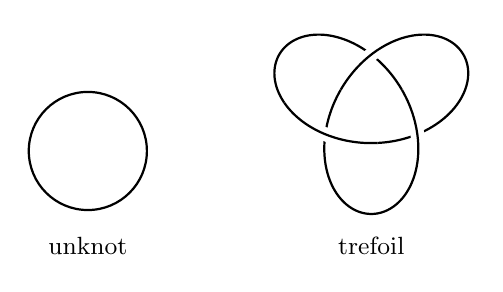
\begin{tikzpicture}[scale=1]
	\draw[thick] (0,0) circle (0.75);
	\node at (0,-1.2) {\small unknot};
	\begin{scope}[xshift=3.6cm, yshift=0.55cm, scale=0.45]
		\foreach \a/\b in {240/360, 0/120, 120/240, 325/362} {
			\draw[white, line width=5pt, samples=90, smooth, variable=\t, domain=\a:\b]
				plot ({sin(\t) + 2*sin(2*\t)}, {cos(\t) - 2*cos(2*\t)});
			\draw[thick, samples=90, smooth, variable=\t, domain=\a:\b]
				plot ({sin(\t) + 2*sin(2*\t)}, {cos(\t) - 2*cos(2*\t)});
		}
		\node at (0,-3.9) {\small trefoil};
	\end{scope}
\end{tikzpicture}
\end{center}

\section{Simplicial Complexes} \label{sec:simplicial}

We have squeezed a great deal out of the fundamental group, but it has a fundamental
limitation: it only sees one-dimensional phenomena. We showed that $S^n$ is simply
connected for all $n \geq 2$, so $\pi_1$ cannot tell $S^2$ from $S^3$. To detect
higher-dimensional holes we need a new invariant, and to build it we will first cut our
spaces into triangles.

\subsection{Simplices}

\begin{definition}[Simplex]
	The \vocab{standard $n$-simplex} is
	$$
	\Delta^n = \left\{(x_0,\dots,x_n) \in \R^{n+1} \;\middle|\; x_i \geq 0, \ \sum_{i=0}^n x_i = 1\right\}
	$$
	with the subspace topology.
\end{definition}

So $\Delta^0$ is a point, $\Delta^1$ is homeomorphic to $I$, $\Delta^2$ is a triangle and
$\Delta^3$ is a tetrahedron. Each $\Delta^n$ is closed and bounded in $\R^{n+1}$, hence
compact, and the standard basis vectors $e_0,\dots,e_n$ are its \vocab{vertices}. By
radial projection from the barycentre, $\Delta^n \cong D^n$.

\begin{center}
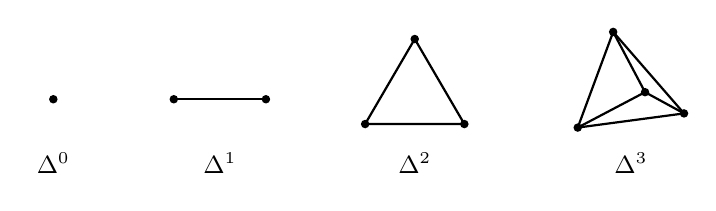
\begin{tikzpicture}[scale=0.9]
	\fill (0,0) circle (0.06);
	\node at (0,-0.9) {\small $\Delta^0$};
	\begin{scope}[xshift=1.7cm]
		\draw[thick] (0,0) -- (1.3,0);
		\fill (0,0) circle (0.06); \fill (1.3,0) circle (0.06);
		\node at (0.65,-0.9) {\small $\Delta^1$};
	\end{scope}
	\begin{scope}[xshift=4.4cm]
		\draw[thick] (0,-0.35) -- (1.4,-0.35) -- (0.7,0.85) -- cycle;
		\fill (0,-0.35) circle (0.06); \fill (1.4,-0.35) circle (0.06); \fill (0.7,0.85) circle (0.06);
		\node at (0.7,-0.9) {\small $\Delta^2$};
	\end{scope}
	\begin{scope}[xshift=7.4cm]
		\draw[thick] (0,-0.4) -- (1.5,-0.2) -- (0.5,0.95) -- cycle;
		\draw[thick] (0,-0.4) -- (0.95,0.1);
		\draw[thick] (1.5,-0.2) -- (0.95,0.1);
		\draw[thick] (0.5,0.95) -- (0.95,0.1);
		\foreach \p in {(0,-0.4), (1.5,-0.2), (0.5,0.95), (0.95,0.1)} { \fill \p circle (0.06); }
		\node at (0.75,-0.9) {\small $\Delta^3$};
	\end{scope}
\end{tikzpicture}
\end{center}

\begin{definition}[Face]
	For $I \subseteq \{0,\dots,n\}$, the \vocab{$I$th face} of $\Delta^n$ is
	$$
	e_I = \{x \in \Delta^n \mid x_i = 0 \text{ for } i \notin I\},
	$$
	and $F(\Delta^n) = \{e_I \mid I \subseteq \{0,\dots,n\}\}$ is the set of faces.
\end{definition}

We abbreviate $I = \{i_0 < \dots < i_k\}$ by the string $i_0i_1\cdots i_k$, so for instance
$e_{02}$ is the edge of $\Delta^2$ joining $e_0$ and $e_2$. Note that
$e_{\{i\}} = e_i$, that $\Delta^n = e_{0\cdots n}$, that $e_\varnothing = \varnothing$,
that $e_I \cong \Delta^{|I|-1}$, and crucially that
$$
e_I \subseteq e_J \iff I \subseteq J, \qquad e_I \cap e_J = e_{I \cap J}.
$$

\begin{definition}
	A map $|f|: \Delta^n \to \R^N$ is \vocab{affine linear} if it is the restriction of a linear map $\R^{n+1}\to\R^N$, equivalently if $|f|(\sum x_ie_i) = \sum x_i |f|(e_i)$. An affine linear map $|f|: \Delta^n \to \Delta^m$ is \vocab{simplicial} if it takes vertices to vertices, so that it is determined by a function $\hat f: \{0,\dots,n\} \to \{0,\dots,m\}$ via $|f|(e_i) = e_{\hat f(i)}$.
\end{definition}

Affine linear maps are continuous and determined by their values on vertices, and a
simplicial map satisfies $|f|(e_I) = e_{\hat f(I)}$.

\begin{definition}[Affine Independence]
	Vectors $v_0,\dots,v_n \in \R^N$ are \vocab{affine linearly independent} if whenever $\sum t_iv_i = 0$ with $\sum t_i = 0$, all $t_i = 0$. Equivalently, $v_1 - v_0, \dots, v_n - v_0$ are linearly independent, or the affine linear map $|f|: \Delta^n \to \R^N$ with $|f|(e_i) = v_i$ is injective.

	In that case we write
	$$
	[v_0,\dots,v_n] = \operatorname{im}|f| = \left\{\sum x_iv_i \;\middle|\; x_i \geq 0, \sum x_i = 1\right\}
	$$
	and call it a \vocab{Euclidean simplex} of dimension $n$.
\end{definition}

Since $\Delta^n$ is compact and $\R^N$ Hausdorff, $|f|: \Delta^n \to [v_0,\dots,v_n]$ is a
homeomorphism. The following lemma says that a Euclidean simplex remembers its vertices,
so `the vertices of $\sigma$' is well-defined; we write $V(\sigma)$ for this set.

\begin{lemma} \label{lem:simplex-vertices}
	For $X \subseteq \R^N$ let $Z(X)$ be the set of $x \in X$ such that whenever $x = \sum t_ix_i$ with $x_i \in X$, $t_i > 0$ and $\sum t_i = 1$, we have $x_i = x$ for some $i$. Then $Z([v_0,\dots,v_n]) = \{v_0,\dots,v_n\}$.
\end{lemma}
\begin{proof}
	If $x$ is not a vertex then $x = \sum x_iv_i$ with at least two $x_i$ positive, and writing $x$ as a convex combination of the $v_i$ involved exhibits $x \notin Z$. Conversely suppose $v_k = \sum_i t_ix_i$ with $t_i > 0$, $\sum t_i = 1$, and write $x_i = \sum_j s_{ij}v_j$ with $s_{ij}\geq 0$ and $\sum_j s_{ij} = 1$. Then
	$$
	v_k = \sum_j \left(\sum_i t_is_{ij}\right)v_j,
	$$
	and $\sum_j\sum_i t_is_{ij} = 1$, so affine independence forces $\sum_i t_is_{ij} = 0$ for $j \neq k$. As $t_i > 0$ and $s_{ij}\geq 0$, we get $s_{ij} = 0$ for all $i$ and $j \neq k$, so every $x_i = v_k$.
\end{proof}

\subsection{Simplicial Complexes}

There are two ways to package a collection of simplices glued along faces --- one
combinatorial, one geometric --- and we shall need both.

\begin{definition}[Abstract Simplicial Complex]
	An \vocab{abstract simplicial complex} in $\Delta^n$ is a subset $K \subseteq F(\Delta^n)$ which is downward closed: if $e_J \in K$ and $I \subseteq J$ then $e_I \in K$.

	Its \vocab{polyhedron} is $|K| = \bigcup_{e_I \in K} e_I \subseteq \Delta^n$, with the subspace topology, and its \vocab{$r$-skeleton} is $K_r = \{e_I \in K \mid |I| \leq r+1\}$.
\end{definition}

Abstract simplicial complexes carry no topology themselves; the topology lives on the
polyhedron, which is compact and Hausdorff. We have a filtration
$\{e_\varnothing\} = K_{-1} \subseteq K_0 \subseteq \dots \subseteq K_n = K$, and
$\dim K$ is the largest $r$ with $K_r \neq K_{r-1}$.

\begin{example} \label{ex:bdelta}
	$\bDelta^n = F(\Delta^n)$ is an abstract simplicial complex with $|\bDelta^n| = \Delta^n \cong D^n$.
\end{example}

\begin{example} \label{ex:ssphere}
	$\sS^{n-1} = \bDelta^n_{n-1} = \{e_I \mid I \subsetneq \{0,\dots,n\}\}$, obtained by throwing away the top face, is an abstract simplicial complex with polyhedron $\partial \Delta^n \cong S^{n-1}$: the boundary of the tetrahedron is a sphere.
\end{example}

\begin{definition}
	A \vocab{simplicial map} $f: K \to L$ between abstract simplicial complexes in $\Delta^n$ and $\Delta^m$ is a map induced by some $\hat f: \{0,\dots,n\}\to\{0,\dots,m\}$ with the property that $e_I \in K$ implies $e_{\hat f(I)} \in L$; then $f(e_I) = e_{\hat f(I)}$. It is a \vocab{simplicial isomorphism} if it is a bijection, in which case $|f|: |K|\to|L|$ is a homeomorphism.
\end{definition}

For the geometric version we work inside $\R^N$. Write $\mathcal{S}(\R^N)$ for the set of
Euclidean simplices in $\R^N$.

\begin{definition}[Euclidean Simplicial Complex]
	A finite set $K \subseteq \mathcal S(\R^N)$ is a \vocab{Euclidean simplicial complex} if
	\begin{enumerate}
		\item $\sigma \in K$ and $\tau$ a face of $\sigma$ implies $\tau \in K$;
		\item $\sigma_1, \sigma_2 \in K$ implies $\sigma_1 \cap \sigma_2$ is a face of each (and so lies in $K$).
	\end{enumerate}
	Its polyhedron is $|K| = \bigcup_{\sigma\in K}\sigma \subseteq \R^N$ and its $r$-skeleton is $K_r = \{\sigma \in K \mid \dim\sigma \leq r\}$.
\end{definition}

Condition (ii) is the one that does the work: it forbids the two configurations on the
right below, in which simplices meet in something which is not a common face.

\begin{center}
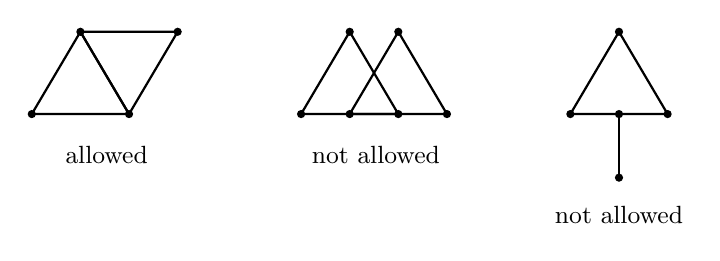
\begin{tikzpicture}[scale=0.95]
	\draw[thick] (0,0) -- (1.3,0) -- (0.65,1.1) -- cycle;
	\draw[thick] (1.3,0) -- (0.65,1.1) -- (1.95,1.1) -- cycle;
	\foreach \p in {(0,0),(1.3,0),(0.65,1.1),(1.95,1.1)} { \fill \p circle (0.055); }
	\node at (1.0,-0.55) {\small allowed};
	\begin{scope}[xshift=3.6cm]
		\draw[thick] (0,0) -- (1.3,0) -- (0.65,1.1) -- cycle;
		\draw[thick] (0.65,0) -- (1.95,0) -- (1.3,1.1) -- cycle;
		\foreach \p in {(0,0),(1.3,0),(0.65,1.1),(0.65,0),(1.95,0),(1.3,1.1)} { \fill \p circle (0.055); }
		\node at (1.0,-0.55) {\small not allowed};
	\end{scope}
	\begin{scope}[xshift=7.2cm]
		\draw[thick] (0,0) -- (1.3,0) -- (0.65,1.1) -- cycle;
		\draw[thick] (0.65,0) -- (0.65,-0.85);
		\foreach \p in {(0,0),(1.3,0),(0.65,1.1),(0.65,0),(0.65,-0.85)} { \fill \p circle (0.055); }
		\node at (0.65,-1.35) {\small not allowed};
	\end{scope}
\end{tikzpicture}
\end{center}

The two notions are equivalent, in the following sense.

\begin{definition}
	Let $K'$ be an abstract simplicial complex in $\Delta^n$ and $|\varphi|: \Delta^n \to \R^N$ affine linear with $|\varphi|$ injective on $|K'|$. Then $\varphi(K') = \{|\varphi|(e_I) \mid e_I \in K'\}$ is called a \vocab{realisation} of $K'$.
\end{definition}

\begin{proposition} \label{prop:realisation}
	A realisation $\varphi(K')$ is a Euclidean simplicial complex, and $|\varphi|: |K'| \to |\varphi(K')|$ is a homeomorphism. Conversely, every Euclidean simplicial complex is a realisation of some abstract simplicial complex, uniquely up to simplicial isomorphism.
\end{proposition}
\begin{proof}
	For the first part, downward closure is inherited from $K'$, and for intersections, injectivity gives
	$$
	|\varphi|(e_{I_1}) \cap |\varphi|(e_{I_2}) = |\varphi|(e_{I_1}\cap e_{I_2}) = |\varphi|(e_{I_1\cap I_2}),
	$$
	which is a common face. That $|\varphi|$ is a homeomorphism follows from compactness of $|K'|$.

	Conversely, let $K$ be a Euclidean simplicial complex, and write its vertex set as $V(K) = \{v_0,\dots,v_n\}$. Define
	$$
	K' = \{e_{i_0\cdots i_k} \in F(\Delta^n) \mid [v_{i_0},\dots,v_{i_k}] \in K\}
	$$
	and let $|\varphi|(e_i) = v_i$. We must check $|\varphi|$ is injective on $|K'|$. It is injective on each $e_I \in K'$, since the corresponding $v_i$ are affine independent. Suppose $|\varphi|(p) = |\varphi|(q) = x$ with $p \in e_I$, $q \in e_J$, both in $K'$. Then $x$ lies in $|\varphi|(e_I)\cap|\varphi|(e_J)$, which is a common face $|\varphi|(e_{I'})$ with $I' \subseteq I \cap J$; by injectivity on $e_I$ and on $e_J$ we get $p, q \in e_{I'}$, and then $p = q$ by injectivity on $e_{I'}$.
\end{proof}

\begin{definition}
	For a Euclidean simplex $\sigma$ of dimension $n$, its \vocab{boundary complex} is $\partial\sigma = F(\sigma)\setminus\{\sigma\}$, with polyhedron $|\partial\sigma| \cong S^{n-1}$. The \vocab{open simplex} is $\sigma^\circ = \sigma \setminus |\partial\sigma|$.
\end{definition}

\begin{lemma} \label{lem:unique-open-simplex}
	Let $K$ be a simplicial complex and $x \in |K|$. Then there is a unique $\sigma \in K$ with $x \in \sigma^\circ$.
\end{lemma}
\begin{proof}
	Work in the abstract picture, where $x \in \Delta^n$. Set $I = \{i \mid x_i \neq 0\}$. Then $x \in e_I^\circ$, and $x \in e_J$ if and only if $I \subseteq J$, which gives both existence and uniqueness; and $e_I \in K$ by downward closure, since $x \in e_J$ for some $e_J \in K$.
\end{proof}

So the open simplices of $K$ partition $|K|$.

\subsection{Barycentric Subdivision}

Simplicial maps are very rigid: there are only finitely many of them between two given
complexes, so most continuous maps $|K|\to|L|$ are not simplicial. The remedy is to chop
$K$ into finer and finer pieces, and the standard way to do this is barycentric
subdivision. We first need cones.

\begin{definition}
	Let $X \subseteq \R^N$ and $p \in \R^N$. We say $p$ is \vocab{independent} of $X$ if for every $x \in X$ the ray from $p$ through $x$ meets $X$ only at $x$. In that case the \vocab{cone} is
	$$
	C_p(X) = \{tp + (1-t)x \mid t \in [0,1],\ x \in X\},
	$$
	and for a Euclidean simplicial complex $K$ with $p$ independent of $|K|$ we set
	$$
	C_p(K) = K \cup \{[v_0,\dots,v_j,p] \mid [v_0,\dots,v_j]\in K\}.
	$$
\end{definition}

\begin{lemma} \label{lem:cone}
	If $p$ is independent of $|K|$ then $C_p(K)$ is a Euclidean simplicial complex with $|C_p(K)| = C_p(|K|)$, and every $\sigma \in C_p(K)$ satisfies $\sigma \cap |K| \in K$.
\end{lemma}

\begin{definition}[Barycentre]
	The \vocab{barycentre} of $\sigma = [v_0,\dots,v_n]$ is $b_\sigma = \frac{1}{n+1}\sum_{i=0}^n v_i$.
\end{definition}

One checks that $b_\sigma$ is independent of $|\partial\sigma|$ and that
$C_{b_\sigma}(|\partial\sigma|) = \sigma$. We may now define barycentric subdivision by a
simultaneous induction on dimension: for a simplex $\sigma$ we set
$$
\beta(\sigma) = C_{b_\sigma}(\bary(\partial\sigma)),
$$
and for a Euclidean simplicial complex $K$ we set
$$
\bary(K) = \bigcup_{\sigma \in K}\beta(\sigma),
$$
starting from $\beta(\varnothing) = \{\varnothing\}$ and $\bary(\{\varnothing\}) = \{\varnothing\}$.
In words: subdivide the boundary, then cone off from the barycentre.

\begin{theorem} \label{thm:subdivision}
	For every $n$ and every $n$-dimensional Euclidean simplex $\sigma$ and $n$-dimensional Euclidean simplicial complex $K$:
	\begin{enumerate}
		\item $\beta(\sigma)$ is an $n$-dimensional Euclidean simplicial complex with $|\beta(\sigma)| = \sigma$, and if $\tau$ is a face of $\sigma$ and $\sigma_1 \in \beta(\sigma)$ then $\sigma_1 \cap \tau \in \beta(\tau)$;
		\item $\bary(K)$ is an $n$-dimensional Euclidean simplicial complex with $|\bary(K)| = |K|$.
	\end{enumerate}
\end{theorem}
\begin{proof}
	Both hold trivially in dimension $-1$. Assume both in dimensions $< n$.

	(i) Now $\partial\sigma$ has dimension $n-1$, so $\bary(\partial\sigma)$ is a Euclidean simplicial complex with polyhedron $|\partial\sigma|$ by the inductive hypothesis (ii). As $b_\sigma$ is independent of $|\partial\sigma|$, Lemma \ref{lem:cone} says $\beta(\sigma) = C_{b_\sigma}(\bary(\partial\sigma))$ is a Euclidean simplicial complex with polyhedron $C_{b_\sigma}(|\partial\sigma|) = \sigma$. The last claim also follows from Lemma \ref{lem:cone}.

	(ii) $\bary(K)$ is finite, and downward closed since each $\beta(\sigma)$ is. For intersections, let $\sigma_i \in \beta(\sigma_i')$ with $\sigma_i' \in K$. Then $\sigma_1 \cap \sigma_2 \subseteq \sigma_1' \cap \sigma_2' = \tau \in K$. By (i), $\sigma_i \cap \tau \in \beta(\tau)$, and $\beta(\tau)$ is a simplicial complex, so
	$$
	\sigma_1\cap\sigma_2 = (\sigma_1\cap\tau)\cap(\sigma_2\cap\tau) \in \beta(\tau) \subseteq \bary(K).
	$$
	Finally $|\bary(K)| = \bigcup_{\sigma\in K}|\beta(\sigma)| = \bigcup_{\sigma\in K}\sigma = |K|$.
\end{proof}

\begin{center}
\begin{tikzpicture}[scale=1.5]
	% original
	\draw[thick] (0,0) -- (1.4,0) -- (0.7,1.21) -- cycle;
	\node at (0.7,-0.4) {\small $\sigma$};
	% first subdivision
	\begin{scope}[xshift=2.3cm]
		\coordinate (A) at (0,0); \coordinate (B) at (1.4,0); \coordinate (C) at (0.7,1.21);
		\coordinate (M) at (0.7,0); \coordinate (N) at (1.05,0.605); \coordinate (P) at (0.35,0.605);
		\coordinate (G) at (0.7,0.4033);
		\draw[thick] (A) -- (B) -- (C) -- cycle;
		\draw[thin, color=blue] (A) -- (G) -- (B); \draw[thin, color=blue] (C) -- (G);
		\draw[thin, color=blue] (M) -- (G) -- (N); \draw[thin, color=blue] (P) -- (G);
		\fill (G) circle (0.035);
		\node at (0.7,-0.4) {\small $\beta(\sigma)$};
	\end{scope}
	% second subdivision
	\begin{scope}[xshift=4.6cm]
		\coordinate (A) at (0,0); \coordinate (B) at (1.4,0); \coordinate (C) at (0.7,1.21);
		\coordinate (G) at (0.7,0.40333);
		\coordinate (Mab) at (0.7,0); \coordinate (Mbc) at (1.05,0.605); \coordinate (Mca) at (0.35,0.605);
		\draw[thick] (A) -- (B) -- (C) -- cycle;
		\draw[thin, color=blue] (A) -- (G); \draw[thin, color=blue] (B) -- (G); \draw[thin, color=blue] (C) -- (G);
		\draw[thin, color=blue] (Mab) -- (G); \draw[thin, color=blue] (Mbc) -- (G); \draw[thin, color=blue] (Mca) -- (G);
		\foreach \X/\Y in {A/Mab, Mab/B, B/Mbc, Mbc/C, C/Mca, Mca/A} {
			\coordinate (mxy) at ($(\X)!0.5!(\Y)$);
			\coordinate (gg) at ($(mxy)!0.33333!(G)$);
			\draw[thin, color=blue] (\X) -- (gg);
			\draw[thin, color=blue] (\Y) -- (gg);
			\draw[thin, color=blue] (G) -- (gg);
			\draw[thin, color=blue] (mxy) -- (gg);
			\draw[thin, color=blue] ($(\Y)!0.5!(G)$) -- (gg);
			\draw[thin, color=blue] ($(G)!0.5!(\X)$) -- (gg);
		}
		\node at (0.7,-0.4) {\small $\bary^2(\sigma)$};
	\end{scope}
\end{tikzpicture}
\end{center}

The reason for subdividing is that the pieces get smaller, and we can quantify this.

\begin{definition}[Mesh]
	The \vocab{mesh} of a Euclidean simplex $\sigma$ is $\mu(\sigma) = \max_{v_i,v_j \in V(\sigma)}\norm{v_i-v_j}$, and $\mu(K) = \max_{\sigma\in K}\mu(\sigma)$.
\end{definition}

\begin{lemma} \label{lem:mesh-max}
	If $\sigma$ is a Euclidean simplex and $x, v \in \sigma$ then $\norm{v-x}\leq \max_{v_i \in V(\sigma)}\norm{v-v_i}$. Consequently $\mu(\sigma) = \max_{x,v\in\sigma}\norm{v-x}$.
\end{lemma}
\begin{proof}
	Write $x = \sum x_iv_i$ with $x_i \geq 0$ and $\sum x_i = 1$; then $v = \sum x_i v$, so
	$$
	\norm{v - x} = \left\|\sum x_i(v-v_i)\right\| \leq \sum x_i\norm{v-v_i} \leq \max_i \norm{v-v_i}. \qedhere
	$$
\end{proof}

\begin{corollary} \label{cor:mesh}
	If $\dim\sigma = n$ then $\mu(\beta(\sigma)) \leq \frac{n}{n+1}\mu(\sigma)$, and if $\dim K = n$ then $\mu(\bary(K))\leq\frac{n}{n+1}\mu(K)$. Hence $\mu(\bary^r(K)) \to 0$ as $r \to \infty$.
\end{corollary}
\begin{proof}
	First, for $\sigma = [v_0,\dots,v_n]$ and any $v \in \sigma$, applying Lemma \ref{lem:mesh-max},
	$$
	\norm{b_\sigma - v} \leq \max_i \norm{b_\sigma - v_i} = \max_i \frac{1}{n+1}\left\|\sum_{j\neq i}(v_j - v_i)\right\| \leq \frac{n}{n+1}\mu(\sigma).
	$$
	Now let $\tau \in \beta(\sigma)$. If $\tau \in \bary(\partial\sigma)$ then by induction $\mu(\tau)\leq\frac{n-1}{n}\mu(\partial\sigma)\leq\frac{n}{n+1}\mu(\sigma)$. Otherwise $\tau = [w_0,\dots,w_k,b_\sigma]$ with $[w_0,\dots,w_k] \in \bary(\partial\sigma)$, and the distance between any two of its vertices is at most $\max\{\frac{n-1}{n}\mu(\sigma), \frac{n}{n+1}\mu(\sigma)\} = \frac{n}{n+1}\mu(\sigma)$. The statement for complexes follows by taking maxima, and iterating gives $\mu(\bary^r(K)) \leq (\frac{n}{n+1})^r\mu(K) \to 0$.
\end{proof}

\subsection{Simplicial Approximation}

We can now say what it means for a simplicial map to approximate a continuous one.

\begin{definition}[Star]
	Let $K$ be a simplicial complex and $v \in V(K)$. The \vocab{star} of $v$ is
	$$
	\St_K(v) = \bigcup_{\{\sigma \in K \,\mid\, v \in V(\sigma)\}} \sigma^\circ.
	$$
\end{definition}

\begin{center}
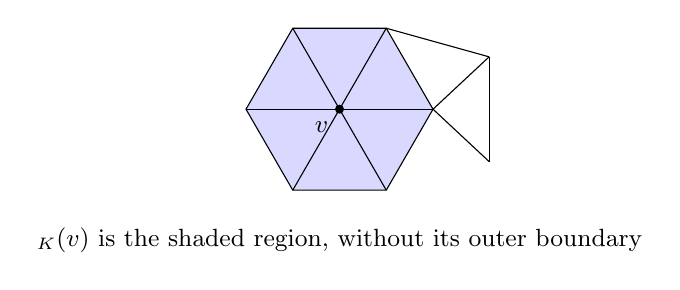
\begin{tikzpicture}[scale=0.95]
	\coordinate (v) at (0,0);
	\foreach \a in {0,60,...,300} { \coordinate (P\a) at (\a:1.25); }
	\fill[color=blue!15] (P0) -- (P60) -- (P120) -- (P180) -- (P240) -- (P300) -- cycle;
	\foreach \a in {0,60,...,300} { \draw[thin] (v) -- (P\a); }
	\draw[thin] (P0) -- (P60) -- (P120) -- (P180) -- (P240) -- (P300) -- cycle;
	\draw[thin] (P0) -- (2.0,0.7); \draw[thin] (P0) -- (2.0,-0.7); \draw[thin] (2.0,0.7) -- (2.0,-0.7);
	\draw[thin] (P60) -- (2.0,0.7);
	\fill (v) circle (0.06);
	\node[below left] at (-0.02,-0.04) {\small $v$};
	\node at (0.0,-1.75) {\small $\St_K(v)$ is the shaded region, without its outer boundary};
\end{tikzpicture}
\end{center}

\begin{lemma} \label{lem:star}
	Let $K$ be a simplicial complex.
	\begin{enumerate}
		\item If $x \in \sigma^\circ$ for $\sigma \in K$, then $x \in \St_K(v)$ if and only if $v \in V(\sigma)$.
		\item $\St_K(v) = |K| \setminus \bigcup\{\sigma \in K \mid v \notin V(\sigma)\}$, so it is open in $|K|$.
		\item $\{\St_K(v) \mid v \in V(K)\}$ is an open cover of $|K|$.
	\end{enumerate}
\end{lemma}
\begin{proof}
	(i) is immediate from Lemma \ref{lem:unique-open-simplex}. For (ii), by (i) the complement of $\St_K(v)$ consists of the open simplices $\sigma^\circ$ with $v \notin V(\sigma)$; and the union of these equals the union of the corresponding closed simplices, since faces of a simplex not containing $v$ also do not contain $v$. That union is a finite union of compact sets, hence closed. (iii) follows since every $x$ lies in some $\sigma^\circ$, and $\sigma$ has at least one vertex.
\end{proof}

\begin{definition}[Simplicial Approximation]
	Let $K, L$ be simplicial complexes and $f: |K| \to |L|$ continuous. A function $\hat g: V(K) \to V(L)$ is a \vocab{simplicial approximation} to $f$ if
	$$
	f(\St_K(v)) \subseteq \St_L(\hat g(v)) \quad\text{for all } v \in V(K).
	$$
\end{definition}

\begin{theorem} \label{thm:approx-is-simplicial}
	If $\hat g$ is a simplicial approximation to $f: |K|\to|L|$, then $\hat g$ determines a simplicial map $g: K \to L$, and $|g| \simeq f$.
\end{theorem}
\begin{proof}
	Let $\sigma \in K$ and pick $x \in \sigma^\circ$; say $f(x) \in \tau^\circ$ with $\tau \in L$. Since $x \in \St_K(v)$ for every $v \in V(\sigma)$, we get
	$$
	f(x) \in \bigcap_{v \in V(\sigma)} f(\St_K(v)) \subseteq \bigcap_{v\in V(\sigma)}\St_L(\hat g(v)),
	$$
	and by Lemma \ref{lem:star}(i) this says $\hat g(v) \in V(\tau)$ for every $v \in V(\sigma)$. So the affine linear extension $|g|$ maps $\sigma$ into $\tau$, and $|g|(\sigma)$ is a face of $\tau$, hence lies in $L$. So $g$ is simplicial.

	For the homotopy, define $H: |K|\times I \to \R^M$ by $H(x,t) = t|g|(x) + (1-t)f(x)$. This is continuous, and we claim it lands in $|L|$. With $x, \sigma, \tau$ as above, $|g|(x) = \sum_i x_i|g|(v_i) \in \tau$ since each $|g|(v_i) \in V(\tau)$, and $f(x) \in \tau$; as $\tau$ is convex, $H(x,t)\in\tau \subseteq |L|$. So $H$ is a homotopy $f \simeq |g|$ in $|L|$.
\end{proof}

\begin{theorem}[Simplicial Approximation Theorem] \label{thm:sat}
	Let $K, L$ be simplicial complexes and $f: |K| \to |L|$ continuous. Then there exist $r \geq 0$ and a simplicial map $g: \bary^r(K) \to L$ with $|g| \simeq f$.
\end{theorem}
\begin{proof}
	By Lemma \ref{lem:star}, $\{\St_L(w) \mid w \in V(L)\}$ is an open cover of $|L|$, so
	$$
	\{f^{-1}(\St_L(w)) \mid w \in V(L)\}
	$$
	is an open cover of $|K|$. Now $|K|$ is a compact metric space, so the Lebesgue covering lemma gives $\delta > 0$ such that each $B_\delta(x)$ lies in some $f^{-1}(\St_L(w_x))$.

	By Corollary \ref{cor:mesh}, choose $r$ with $\mu(\bary^r(K)) < \delta$ and put $K' = \bary^r(K)$, noting $|K'| = |K|$. If $x \in V(K')$ and $\sigma \in K'$ has $x \in V(\sigma)$ then $\sigma \subseteq B_\delta(x)$, since every point of $\sigma$ is within $\mu(K') < \delta$ of $x$. Hence
	$$
	\St_{K'}(x) \subseteq \bigcup_{\{\sigma \,\mid\, x \in V(\sigma)\}}\sigma \subseteq B_\delta(x),
	$$
	so $f(\St_{K'}(x)) \subseteq f(B_\delta(x)) \subseteq \St_L(w_x)$. Therefore $\hat g(x) = w_x$ defines a simplicial approximation to $f$, and Theorem \ref{thm:approx-is-simplicial} does the rest.
\end{proof}

This is the technical engine of everything to come. Here is a first payoff, which already
does something the fundamental group could not.

\begin{corollary} \label{cor:not-surjective}
	Let $K, L$ be simplicial complexes with $\dim K < \dim L$, and let $f: |K|\to|L|$ be continuous. Then $f \simeq |g|$ for some $|g|$ which is not surjective.
\end{corollary}
\begin{proof}
	Take a simplicial $g: \bary^r(K)\to L$ with $|g|\simeq f$. Simplicial maps do not raise dimension, so $|g|$ has image in $|L_k|$ where $k = \dim\bary^r(K) = \dim K < \dim L$. As $|L_k| \subsetneq |L|$, this is not surjective.
\end{proof}

\begin{theorem} \label{thm:sk-to-sn}
	If $k < n$, every map $S^k \to S^n$ is null-homotopic.
\end{theorem}
\begin{proof}
	We have $S^k \cong |\sS^k|$ and $S^n \cong |\sS^n|$ with $\dim \sS^k = k < n = \dim\sS^n$, so by Corollary \ref{cor:not-surjective}, $f \simeq |g|$ where $|g|$ misses some point $p \in S^n$. But then $|g|$ factors through $S^n\setminus\{p\}\cong\R^n$, which is contractible, so $|g|$ is null-homotopic; hence so is $f$.
\end{proof}

That gives one half of the statement $S^n \simeq S^m \implies n = m$: any map $S^k \to S^n$
with $k < n$ is null-homotopic, whereas we would need $\id_{S^n}$ not to be. To prove
the latter we need homology.

\section{Simplicial Homology}

Here is the idea. Having chopped a space into simplices, we form for each $k$ the free
abelian group on the $k$-simplices, and a boundary homomorphism $d$ taking a simplex to
the (signed) sum of its faces. A $k$-dimensional hole should be a $k$-cycle --- something
with no boundary --- which is not itself the boundary of anything. Measuring how badly
`no boundary' fails to imply `is a boundary' is exactly taking a quotient group, and that
quotient is homology.

\subsection{Chain Complexes}

\begin{definition}[Chain Complex]
	A \vocab{chain complex} $(C_\bullet, d)$ consists of
	\begin{enumerate}
		\item free abelian groups $C_i$ for $i \in \Z$, all but finitely many of which are zero;
		\item homomorphisms $d_i: C_i \to C_{i-1}$;
		\item such that $d_{i-1}\circ d_i = 0$ for all $i$.
	\end{enumerate}
	\[\begin{tikzcd}[column sep=small]
		\cdots \arrow[r] & {C_{i+1}} \arrow[r, "{d_{i+1}}"] & {C_i} \arrow[r, "{d_i}"] & {C_{i-1}} \arrow[r] & \cdots
	\end{tikzcd}\]
\end{definition}

We write $C_\bullet = \bigoplus_i C_i$ and $d = \bigoplus_i d_i$, so that condition (iii)
says exactly $d^2 = 0$.

\begin{definition}
	Let $x \in C_k$. We say $x$ is a \vocab{cycle} if $dx = 0$, and a \vocab{boundary} if $x = dy$ for some $y \in C_{k+1}$.
\end{definition}

Since $d^2 = 0$, every boundary is a cycle: $\operatorname{im}d_{k+1} \subseteq \ker d_k$.
The whole subject consists of measuring the failure of the converse.

Now we build the chain complex of a simplicial complex. Let $K$ be an abstract simplicial
complex in $\Delta^n$.

\begin{definition}[Simplicial Chain Complex]
	The \vocab{reduced chain group} is the free abelian group
	$$
	\widetilde C_k(K) = \genby{e_I \mid e_I \in K, \ |I| = k+1},
	$$
	with boundary map defined on basis elements by
	$$
	d(e_I) = \sum_{j=0}^{k}(-1)^j e_{I_{\hat\jmath}}, \qquad I_{\hat\jmath} = I \setminus \{i_j\},
	$$
	where $I = i_0i_1\cdots i_k$ with $i_0 < \dots < i_k$.
\end{definition}

Note that $\widetilde C_{-1}(K) = \genby{e_\varnothing} \cong \Z$, generated by the empty
face, and $d(e_i) = e_\varnothing$ for each vertex. The \vocab{unreduced} chain complex
$C_\bullet(K)$ is obtained by throwing this away: $C_k(K) = \widetilde C_k(K)$ for
$k \geq 0$ and $C_{-1}(K) = 0$, with the same $d$.

The alternating signs are what makes everything work.

\begin{proposition}
	$d^2 = 0$.
\end{proposition}
\begin{proof}
	It suffices to check this on basis elements. Expanding,
	$$
	d^2(e_I) = \sum_{j < j'} c_{jj'}\, e_{I_{\hat\jmath\hat\jmath'}},
	$$
	where $I_{\hat\jmath\hat\jmath'} = I \setminus \{i_j, i_{j'}\}$. There are two ways to arrive at this term: deleting $i_j$ first and then $i_{j'}$, which now sits in position $j'-1$, contributing $(-1)^j(-1)^{j'-1}$; or deleting $i_{j'}$ first and then $i_j$, still in position $j$, contributing $(-1)^{j'}(-1)^j$. So
	$$
	c_{jj'} = (-1)^{j+j'-1} + (-1)^{j+j'} = 0. \qedhere
	$$
\end{proof}

\begin{example} \label{ex:chain-delta2}
	Take $K = \bDelta^2$, the full triangle. Then
	$$
	\widetilde C_2 = \genby{e_{012}},\quad \widetilde C_1 = \genby{e_{01},e_{02},e_{12}},\quad \widetilde C_0 = \genby{e_0,e_1,e_2},\quad \widetilde C_{-1} = \genby{e_\varnothing},
	$$
	and all other $\widetilde C_i = 0$. The boundary maps are
	$$
	d(e_{012}) = e_{12}-e_{02}+e_{01}, \quad d(e_{01}) = e_1-e_0,\quad d(e_{02}) = e_2 - e_0, \quad d(e_{12}) = e_2 - e_1,
	$$
	and $d(e_i) = e_\varnothing$. As a check,
	$$
	d^2(e_{012}) = (e_2-e_1)-(e_2-e_0)+(e_1-e_0) = 0.
	$$
\end{example}

The signs encode orientations: $e_{01}$ is the edge from $e_0$ to $e_1$, and
$d(e_{012}) = e_{01} - e_{02} + e_{12}$ traverses the boundary of the triangle
consistently anticlockwise.

\begin{center}
\begin{tikzpicture}[scale=1.5]
	\coordinate (A) at (0,0); \coordinate (B) at (1.5,0); \coordinate (C) at (0.75,1.3);
	\draw[thick] (A) -- (B) -- (C) -- cycle;
	\draw[->, very thick, color=blue] ($(A)!0.45!(B)$) -- ($(A)!0.58!(B)$);
	\draw[->, very thick, color=blue] ($(B)!0.45!(C)$) -- ($(B)!0.58!(C)$);
	\draw[->, very thick, color=blue] ($(C)!0.45!(A)$) -- ($(C)!0.58!(A)$);
	\fill (A) circle (0.045); \fill (B) circle (0.045); \fill (C) circle (0.045);
	\node[below left] at (A) {\small $e_0$};
	\node[below right] at (B) {\small $e_1$};
	\node[above] at (C) {\small $e_2$};
	\node[below] at ($(A)!0.25!(B)$) {\small $e_{01}$};
	\node[right] at ($(B)!0.78!(C)$) {\small $e_{12}$};
	\node[left] at ($(A)!0.78!(C)$) {\small $e_{02}$};
	\node at (0.75,0.45) {\small $e_{012}$};
\end{tikzpicture}
\end{center}

\subsection{Homology Groups}

\begin{definition}[Homology]
	Let $(C_\bullet, d)$ be a chain complex. Its \vocab{$k$th homology group} is
	$$
	H_k(C_\bullet) = \frac{\ker d_k}{\operatorname{im} d_{k+1}}.
	$$
	For a simplicial complex $K$ we set $H_k(K) = H_k(C_\bullet(K))$ and
	$\widetilde H_k(K) = H_k(\widetilde C_\bullet(K))$, the \vocab{reduced homology}.
\end{definition}

Homology groups are abelian, being quotients of subgroups of free abelian groups. For
$x \in \ker d$ we write $[x]$ for its class in $H_\bullet$.

\begin{example} \label{ex:homology-delta2}
	Continuing Example \ref{ex:chain-delta2}, let us compute $\widetilde H_\bullet(\bDelta^2)$.
	\begin{itemize}
		\item $d_2$ is injective, so $\ker d_2 = 0$ and $\widetilde H_2 = 0$.
		\item For $x = ae_{01}+be_{12}+ce_{02}$ we have $dx = -(a+c)e_0 + (a-b)e_1 + (b+c)e_2$, so $dx = 0$ iff $a = b = -c$. Hence $\ker d_1 = \genby{e_{01}+e_{12}-e_{02}} = \operatorname{im}d_2$, giving $\widetilde H_1 = 0$.
		\item $\ker d_0 = \{ae_0+be_1+ce_2 \mid a+b+c = 0\}$, which is spanned by $e_1-e_0, e_2-e_0$, and these lie in $\operatorname{im}d_1$. So $\widetilde H_0 = 0$.
		\item $d_0$ is surjective onto $\widetilde C_{-1}$, so $\widetilde H_{-1} = 0$.
	\end{itemize}
	So all the reduced homology of the full triangle vanishes. Passing to unreduced homology only changes degree $0$:
	$$
	H_k(\bDelta^2) = \begin{cases}\Z & k = 0\\ 0 & \text{otherwise.}\end{cases}
	$$
\end{example}

\begin{example} \label{ex:homology-points}
	Let $K = \{e_\varnothing, e_0, \dots, e_r\}$, so $|K|$ is $r+1$ points. Then $\widetilde C_i(K) = 0$ for $i > 0$, and $\ker d_0 = \genby{e_1-e_0,\dots,e_r-e_0} \cong \Z^r$ with $\operatorname{im}d_1 = 0$. So $\widetilde H_0(K) \cong \Z^r$ and $H_0(K) \cong \Z^{r+1}$.
\end{example}

That is a general phenomenon: $H_0$ counts path components, while $\widetilde H_0$ counts
them minus one.

\begin{example}[The Circle] \label{ex:homology-circle}
	Let $T_n$ be the boundary of a convex $n$-gon, realising the abstract complex
	$$
	K = \{e_\varnothing, e_0,\dots,e_{n-1}, e_{01},e_{12},\dots,e_{(n-2)(n-1)}, e_{0(n-1)}\},
	$$
	so that $|K| \cong S^1$. Then $C_1(K)$ is free of rank $n$ and $C_0(K)$ is free of rank $n$, with $d(e_{i(i+1)}) = e_{i+1}-e_i$ and $d(e_{0(n-1)}) = e_{n-1}-e_0$. Setting
	$$
	x = e_{01}+e_{12}+\dots+e_{(n-2)(n-1)} - e_{0(n-1)},
	$$
	we get $dx = 0$, and a short computation shows $\ker d_1 = \genby{x}$. As $C_2 = 0$,
	$$
	H_1(K) = \genby{x} \cong \Z.
	$$
	Also $\ker d_0 = C_0$ and $\operatorname{im}d_1$ is spanned by the $e_{i+1}-e_i$, so $H_0(K) \cong \Z$. Note that the answer does not depend on $n$, even though the complexes do --- as it must not, since all the $|T_n|$ are homeomorphic. That homology depends only on $|K|$ is a theorem we will prove in the next section.
\end{example}

\subsection{Chain Maps}

We want simplicial maps to induce maps on homology, and for that we need the notion of a
map of chain complexes.

\begin{definition}[Chain Map]
	Let $(C_\bullet,d)$ and $(C_\bullet',d')$ be chain complexes. A \vocab{chain map} $f: C_\bullet \to C_\bullet'$ is a collection of homomorphisms $f_i: C_i \to C_i'$ with $f_{i-1}\circ d_i = d_i'\circ f_i$, that is, with $fd = d'f$.
\end{definition}

\begin{proposition} \label{prop:chain-map-induces}
	A chain map $f$ induces a homomorphism $f_*: H_\bullet(C) \to H_\bullet(C')$ by $f_*[x] = [f(x)]$, and $(f\circ g)_* = f_*\circ g_*$.
\end{proposition}
\begin{proof}
	If $dx = 0$ then $d'f(x) = f(dx) = 0$, so $f(\ker d)\subseteq \ker d'$; and if $x = dy$ then $f(x) = d'f(y)$, so $f(\operatorname{im}d)\subseteq\operatorname{im}d'$. Hence $f$ descends to the quotients. Functoriality is immediate.
\end{proof}

Now let $f: K \to L$ be a simplicial map, determined by
$\hat f: \{0,\dots,n\}\to\{0,\dots,m\}$. The obvious guess is to define
$f_\sharp(e_I) = e_{\hat f(I)}$, and this fails for two reasons.

First, if $\hat f$ is not injective on $I$ then $e_{\hat f(I)}$ has smaller dimension than
$e_I$: for $f: \bDelta^1 \to \bDelta^1$ with $e_0, e_1 \mapsto e_0$ we would need
$f_\sharp(e_{01}) = e_0$, which does not preserve grading.

Second, the signs go wrong. For $f: \bDelta^1\to\bDelta^1$ swapping $e_0$ and $e_1$, we
would have $f_\sharp(e_{01}) = e_{01}$, so $d f_\sharp(e_{01}) = e_1-e_0$, while
$f_\sharp d(e_{01}) = f_\sharp(e_1 - e_0) = e_0 - e_1$.

The fix for both is to allow \emph{ordered} index tuples and to build the signs in.

\begin{definition}
	For $I = (i_0,\dots,i_k) \in \{0,\dots,n\}^{k+1}$, define $e_I \in \widetilde C_k(\bDelta^n)$ by
	$$
	e_I = \begin{cases}0 & \text{if $I$ has a repeated entry},\\ (-1)^{S(I)}e_{I'} & \text{otherwise},\end{cases}
	$$
	where $I'$ is the increasing rearrangement of $I$ and $(-1)^{S(I)}$ is the sign of the permutation taking $I$ to $I'$.
\end{definition}

So $e_{102} = -e_{012} = e_{210}$ and $e_{001} = 0$. With this convention the boundary
formula holds in general.

\begin{proposition} \label{prop:d-general}
	For any $I \in \{0,\dots,n\}^{k+1}$ we have $d(e_I) = \sum_{j=0}^k(-1)^je_{I_{\hat\jmath}}$, where $I_{\hat\jmath}$ omits the $j$th entry of the tuple.
\end{proposition}
\begin{proof}
	If $I$ has a repeated entry the claim is a direct check: if the repeat is at positions $j_1 \neq j_2$, all terms $e_{I_{\hat\jmath}}$ with $j \notin \{j_1,j_2\}$ vanish, and the remaining two terms cancel by the sign rule. Otherwise let $\sigma$ take $I$ to $I'$; if $i_j$ sits in position $j'$ in $I'$ then removing it changes the number of inversions by $j - j'$, so $S(I_{\hat\jmath}) \equiv S(I) + j - j' \pmod 2$. Hence
	\begin{align*}
	\sum_j (-1)^je_{I_{\hat\jmath}} &= \sum_j (-1)^{j}(-1)^{S(I)+j-j'}e_{(I')_{\hat\jmath'}} \\
	&= (-1)^{S(I)}\sum_{j'}(-1)^{j'}e_{(I')_{\hat\jmath'}} = (-1)^{S(I)}d(e_{I'}) = d(e_I). \qedhere
	\end{align*}
\end{proof}

\begin{definition}
	For a simplicial map $f: K \to L$ define $f_\sharp: C_k(K) \to C_k(L)$ on basis elements by
	$$
	f_\sharp(e_{i_0\cdots i_k}) = e_{\hat f(i_0)\cdots \hat f(i_k)} .
	$$
\end{definition}

This preserves grading, and collapses degenerate images to zero rather than dropping
dimension.

\begin{proposition}
	$f_\sharp$ is a chain map.
\end{proposition}
\begin{proof}
	Using Proposition \ref{prop:d-general} twice,
	$$
	d(f_\sharp(e_I)) = d(e_{\hat f(I)}) = \sum_{j=0}^k(-1)^je_{(\hat f(I))_{\hat\jmath}} = f_\sharp\left(\sum_{j=0}^k(-1)^je_{I_{\hat\jmath}}\right) = f_\sharp(d(e_I)). \qedhere
	$$
\end{proof}

\begin{example}
	For $f: \bDelta^1\to\bDelta^1$ with $e_0,e_1 \mapsto e_0$ we get $f_\sharp(e_{01}) = e_{00} = 0$, and for $f$ the swap we get $f_\sharp(e_{01}) = e_{10} = -e_{01}$, so $df_\sharp(e_{01}) = -(e_1-e_0) = e_0-e_1 = f_\sharp(d e_{01})$. Both problems are fixed.
\end{example}

We write $f_* : H_\bullet(K)\to H_\bullet(L)$ for the induced map on homology.

\subsection{Chain Homotopies}

Homotopic maps of spaces should induce the same map on homology. The algebraic shadow of
a homotopy is the following.

\begin{definition}[Chain Homotopy]
	Chain maps $f_0, f_1: (C,d)\to(C',d')$ are \vocab{chain homotopic}, written $f_0 \simeq f_1$, if there are homomorphisms $h_i: C_i \to C_{i+1}'$ with
	$$
	d'h + hd = f_0 - f_1 .
	$$
	We call $h$ a \vocab{chain homotopy}.
\end{definition}

The formula looks unmotivated until one draws the picture. If $f_0, f_1: X \to Y$ are
homotopic via $H$, then $H$ sweeps each simplex $\sigma$ out into a prism
$\sigma \times I$, and the boundary of that prism consists of the two ends $f_0(\sigma)$
and $f_1(\sigma)$ together with the prism on $\partial\sigma$. Writing $h$ for `sweep out
into a prism', that reads $dh + hd = f_1 - f_0$, up to signs.

\begin{center}
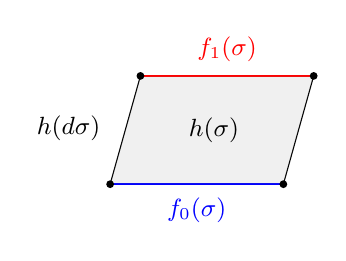
\begin{tikzpicture}[scale=1.1]
	\draw[thick, color=blue] (0,0) -- (2,0);
	\draw[thick, color=red] (0.35,1.25) -- (2.35,1.25);
	\draw[thin] (0,0) -- (0.35,1.25);
	\draw[thin] (2,0) -- (2.35,1.25);
	\fill[color=gray, opacity=0.12] (0,0) -- (2,0) -- (2.35,1.25) -- (0.35,1.25) -- cycle;
	\fill (0,0) circle (0.045); \fill (2,0) circle (0.045);
	\fill (0.35,1.25) circle (0.045); \fill (2.35,1.25) circle (0.045);
	\node[color=blue, below] at (1,-0.05) {\small $f_0(\sigma)$};
	\node[color=red, above] at (1.35,1.3) {\small $f_1(\sigma)$};
	\node at (1.2,0.62) {\small $h(\sigma)$};
	\node[left] at (0.0,0.65) {\small $h(d\sigma)$};
\end{tikzpicture}
\end{center}

\begin{lemma} \label{lem:chain-homotopy}
	If $f_0 \simeq f_1$ then $f_{0*} = f_{1*}: H_\bullet(C)\to H_\bullet(C')$.
\end{lemma}
\begin{proof}
	Let $[x]\in H_\bullet(C)$, so $dx = 0$. Then
	$$
	f_{0*}[x]-f_{1*}[x] = [(f_0-f_1)x] = [(d'h+hd)x] = [d'h(x)] = 0,
	$$
	since $d'h(x) \in \operatorname{im}d'$.
\end{proof}

\begin{definition}
	A chain complex $(C,d)$ is \vocab{contractible} if $\id_C \simeq 0$.
\end{definition}

\begin{lemma} \label{lem:contractible-chain}
	If $(C,d)$ is contractible then $H_\bullet(C) = 0$.
\end{lemma}
\begin{proof}
	$[x] = (\id)_*[x] = 0_*[x] = 0$ for every class.
\end{proof}

The basic example of a contractible chain complex comes from coning off.

\begin{definition}
	Let $K$ be an abstract simplicial complex in $\Delta^n$ not containing the vertex $e_0$. Its \vocab{cone} is $C_{e_0}(K) = K \cup \{e_{0I} \mid e_I \in K\}$, an abstract simplicial complex.
\end{definition}

\begin{proposition} \label{prop:cone-contractible}
	$\widetilde C_\bullet(C_{e_0}(K))$ is contractible, and hence $\widetilde H_\bullet(C_{e_0}(K)) = 0$.
\end{proposition}
\begin{proof}
	Define $h: \widetilde C_k \to \widetilde C_{k+1}$ on basis elements by $h(e_I) = e_{0I}$, noting that this is zero when $0 \in I$. We check $dh + hd = \id$.

	If $0 \notin I$ then by Proposition \ref{prop:d-general},
	$$
	dh(e_I) = d(e_{0I}) = e_I + \sum_{j=0}^{k}(-1)^{j+1}e_{0I_{\hat\jmath}} = e_I - h(d e_I),
	$$
	so $dh(e_I)+hd(e_I) = e_I$. If $0 \in I$, say $I = 0J$ with $0 \notin J$, then $h(e_I) = 0$ so $dh(e_I) = 0$, while
	$$
	hd(e_{0J}) = h\left(e_J - \sum_j (-1)^{j}e_{0J_{\hat\jmath}}\right) = e_{0J} - 0 = e_I,
	$$
	using $h(e_{0J_{\hat\jmath}}) = e_{00J_{\hat\jmath}} = 0$. So $dh+hd = \id$ in both cases.
\end{proof}

\begin{corollary} \label{cor:cone-homology}
	$H_i(C_{e_0}(K)) = \Z$ for $i=0$ and $0$ otherwise. In particular this holds for $\bDelta^n = C_{e_0}(\bDelta^{n}\text{ on } \{1,\dots,n\})$, so a simplex has the homology of a point.
\end{corollary}
\begin{proof}
	Write $(\widetilde C, \widetilde d)$ and $(C,d)$ for the reduced and unreduced complexes. For $i > 0$ we have $\ker \widetilde d_i = \ker d_i$ and $\operatorname{im}\widetilde d_{i+1} = \operatorname{im}d_{i+1}$, so $H_i(C) = \widetilde H_i = 0$. In degree $0$, $\widetilde H_{-1} = 0$ says $\widetilde d_0: \widetilde C_0 \to \genby{e_\varnothing}\cong\Z$ is surjective, and $\widetilde H_0 = 0$ says $\ker\widetilde d_0 = \operatorname{im}\widetilde d_1$. Hence
	$$
	\Z \cong \widetilde C_0/\ker\widetilde d_0 = \widetilde C_0 /\operatorname{im}\widetilde d_1 = C_0/\operatorname{im}d_1 = \ker d_0/\operatorname{im}d_1 = H_0(C). \qedhere
	$$
\end{proof}

\subsection{Exact Sequences}

To compute anything beyond cones we need a way of relating the homology of a space to
that of its pieces. The algebra behind this is the theory of exact sequences.

\begin{definition}[Exact Sequence]
	A sequence of abelian groups and homomorphisms
	\[\begin{tikzcd}[column sep=small]
		\cdots \arrow[r] & {A_{k+1}} \arrow[r, "{f_{k+1}}"] & {A_k} \arrow[r, "{f_k}"] & {A_{k-1}} \arrow[r] & \cdots
	\end{tikzcd}\]
	is \vocab{exact at $A_k$} if $\ker f_k = \operatorname{im}f_{k+1}$, and \vocab{exact} if it is exact everywhere. A \vocab{short exact sequence} is an exact sequence of the form
	\[\begin{tikzcd}[column sep=small]
		0 \arrow[r] & A \arrow[r, "f"] & B \arrow[r, "g"] & C \arrow[r] & 0 .
	\end{tikzcd}\]
\end{definition}

Unwinding: $0 \to A \to B$ is exact at $A$ iff $f$ is injective; $B \to C \to 0$ is exact
at $C$ iff $g$ is surjective; and a short exact sequence says exactly that $f$ is
injective, $g$ is surjective, and $C \cong B/f(A)$.

\begin{definition}
	A \vocab{short exact sequence of chain complexes} is a pair of chain maps
	\[\begin{tikzcd}[column sep=small]
		0 \arrow[r] & {A_\bullet} \arrow[r, "f"] & {B_\bullet} \arrow[r, "g"] & {C_\bullet} \arrow[r] & 0
	\end{tikzcd}\]
	such that $0 \to A_k \to B_k \to C_k \to 0$ is exact for every $k$.
\end{definition}

The following is the engine of every homology computation we will do.

\begin{lemma}[Snake Lemma] \label{lem:snake}
	Given a short exact sequence of chain complexes as above, there are homomorphisms $\partial_k: H_k(C)\to H_{k-1}(A)$, the \vocab{connecting homomorphisms}, such that the sequence
	\[\begin{tikzcd}[column sep=small]
		\cdots \arrow[r] & {H_k(A)} \arrow[r, "{f_*}"] & {H_k(B)} \arrow[r, "{g_*}"] & {H_k(C)} \arrow[r, "{\partial_k}"] & {H_{k-1}(A)} \arrow[r, "{f_*}"] & \cdots
	\end{tikzcd}\]
	is exact. This is the \vocab{long exact sequence} of the short exact sequence.
\end{lemma}
\begin{proof}
	\emph{Construction of $\partial_k$.} Let $[c] \in H_k(C)$, so $dc = 0$.
	\begin{enumerate}
		\item $g$ is surjective, so choose $b \in B_k$ with $g(b) = c$.
		\item $g(db) = d g(b) = dc = 0$, so $db \in \ker g = \operatorname{im}f$; choose $a \in A_{k-1}$ with $f(a) = db$.
		\item $f(da) = d f(a) = d^2 b = 0$, and $f$ is injective, so $da = 0$.
	\end{enumerate}
	We set $\partial_k[c] = [a]$.
	\begin{center}
	\begin{tikzcd}[row sep=large, column sep=small]
		0 \arrow[r] & {A_k} \arrow[r, "f"] \arrow[d, "d"] & {B_k} \arrow[r, "g"] \arrow[d, "d"] & {C_k} \arrow[r] \arrow[d, "d"] \arrow[ld, "{\partial_k}"', dashed, near start] & 0 \\
		0 \arrow[r] & {A_{k-1}} \arrow[r, "f"] & {B_{k-1}} \arrow[r, "g"] & {C_{k-1}} \arrow[r] & 0
	\end{tikzcd}
	\end{center}

	\emph{Well-definedness.} Suppose $g(b') = c$ too. Then $b - b' \in \ker g = \operatorname{im}f$, say $b - b' = f(\alpha)$. Then $f(a) - f(a') = db - db' = f(d\alpha)$, so $a - a' = d\alpha$ by injectivity of $f$, and $[a] = [a']$. Now suppose $[c] = [c']$, so $c - c' = d\gamma$ with $\gamma = g(\beta)$ by surjectivity. Replacing $b$ by $b - d\beta$ we may assume $b$ maps to $c'$, and $d(b - d\beta) = db$, so we get the same $a$.

	\emph{Exactness at $H_k(C)$.} If $\partial_k[c] = 0$ then $a = d\alpha$ for some $\alpha\in A_k$, and then $d(b - f(\alpha)) = db - f(d\alpha) = db - f(a) = 0$, so $[b - f(\alpha)]\in H_k(B)$ and $g_*[b-f(\alpha)] = [g(b)] = [c]$. Conversely if $[c] = g_*[b]$ with $db = 0$ then in the construction we may take $a = 0$.

	\emph{Exactness at $H_k(B)$.} Certainly $g_*f_* = (gf)_* = 0$. Conversely if $g_*[b] = 0$ then $g(b) = d\gamma$ for some $\gamma \in C_{k+1}$, and choosing $\beta$ with $g(\beta) = \gamma$ we get $g(b - d\beta) = 0$, so $b - d\beta = f(\alpha)$ for some $\alpha \in A_k$. Then $f(d\alpha) = d(b-d\beta) = 0$, so $d\alpha = 0$ and $[b] = [b - d\beta] = f_*[\alpha]$.

	\emph{Exactness at $H_{k-1}(A)$.} If $[a] = \partial_k[c]$ then $f_*[a] = [db] = 0$. Conversely if $f_*[a] = 0$ then $f(a) = db$ for some $b \in B_k$, and $dg(b) = g(db) = g(f(a)) = 0$, so $[g(b)] \in H_k(C)$ and by construction $\partial_k[g(b)] = [a]$.
\end{proof}

\subsection{The Mayer--Vietoris Sequence}

Let $K_1, K_2$ be abstract simplicial complexes in $\Delta^n$. Then $K_1\cap K_2$ and
$K_1 \cup K_2$ are also abstract simplicial complexes, and the inclusions give a
commuting square, hence a commuting square of chain maps.

\begin{proposition} \label{prop:mv-ses}
	The sequence
	\[\begin{tikzcd}[column sep=small]
		0 \arrow[r] & {C_\bullet(K_1\cap K_2)} \arrow[r, "i"] & {C_\bullet(K_1)\oplus C_\bullet(K_2)} \arrow[r, "j"] & {C_\bullet(K_1\cup K_2)} \arrow[r] & 0,
	\end{tikzcd}\]
	with $i(x) = (i_{1\sharp}x, i_{2\sharp}x)$ and $j(x,y) = j_{1\sharp}x - j_{2\sharp}y$, is a short exact sequence of chain complexes.
\end{proposition}
\begin{proof}
	Each $C_\bullet(K)$ has as basis the $e_I \in K$, and the maps $i_\sharp, j_\sharp$ send basis elements to basis elements, so we may argue basiswise.

	$i$ is injective since $i_{1\sharp}$ is. Next, $ji = j_{1\sharp}i_{1\sharp} - j_{2\sharp}i_{2\sharp} = 0$ as the square commutes, so $\operatorname{im}i \subseteq \ker j$. Conversely if $j(x,y) = 0$ then $x = y$ as elements of $C_\bullet(K_1\cup K_2)$, so all the simplices occurring lie in both $K_1$ and $K_2$, giving $x = y \in C_\bullet(K_1\cap K_2)$ and $(x,y) = i(x)$.

	Finally, if $e_I \in K_1\cup K_2$ then $e_I \in K_1$ or $e_I \in K_2$, and correspondingly $e_I = j(e_I, 0)$ or $e_I = j(0,-e_I)$. So $j$ is surjective.
\end{proof}

\begin{theorem}[Mayer--Vietoris] \label{thm:mv}
	Let $K_1, K_2$ be abstract simplicial complexes in $\Delta^n$. Then there is a long exact sequence
	\begin{align*}
		\cdots \to H_k(K_1\cap K_2) &\xrightarrow{\ i_*\ } H_k(K_1)\oplus H_k(K_2) \xrightarrow{\ j_*\ } H_k(K_1\cup K_2) \\
		&\xrightarrow{\ \partial_k\ } H_{k-1}(K_1\cap K_2) \xrightarrow{\ i_*\ } H_{k-1}(K_1)\oplus H_{k-1}(K_2) \to \cdots
	\end{align*}
\end{theorem}
\begin{proof}
	Apply the snake lemma to Proposition \ref{prop:mv-ses}.
\end{proof}

\begin{example}[Disjoint Unions] \label{ex:disjoint}
	If $K_1$ and $K_2$ are disjoint complexes inside a common $\Delta^n$, so that $K_1 \cap K_2 = \{e_\varnothing\}$ and hence $C_\bullet(K_1\cap K_2) = 0$, the Mayer--Vietoris sequence degenerates to
	\[\begin{tikzcd}[column sep=small]
		0 \arrow[r] & {H_k(K_1)\oplus H_k(K_2)} \arrow[r] & {H_k(K_1\sqcup K_2)} \arrow[r] & 0,
	\end{tikzcd}\]
	so $H_k(K_1\sqcup K_2) \cong H_k(K_1)\oplus H_k(K_2)$: homology of a disjoint union is the direct sum.
\end{example}

We can already compute the homology of spheres, using nothing but the long exact
sequence.

\begin{theorem} \label{thm:homology-spheres}
	For $n \geq 1$,
	$$
	H_k(\sS^n) = \begin{cases}\Z & k = 0, n\\ 0 & \text{otherwise.}\end{cases}
	$$
\end{theorem}
\begin{proof}
	Recall $\sS^{n} = \bDelta^{n+1}\setminus\{e_{0\cdots(n+1)}\}$ has polyhedron $S^{n}$. We induct on $n$. For $n = 1$ this is Example \ref{ex:homology-circle}, since $|\sS^1|$ is the boundary of a triangle.

	For the inductive step, write $\sS^n = K_1 \cup K_2$ where
	$$
	K_1 = \{e_I \mid I \subseteq \{0,\dots,n\}\}, \qquad K_2 = \{e_I \mid I \subsetneq \{0,\dots,n+1\}, \ I \neq \{0,\dots,n\}\}.
	$$
	Both are downward closed, and their union is all of $\sS^n$. Now $K_1 = \bDelta^n$ is a simplex, while $K_2 = C_{e_{n+1}}(\sS^{n-1})$ is a cone on the vertex $e_{n+1}$, so both have the homology of a point by Corollary \ref{cor:cone-homology}; geometrically these are the two hemispheres. Their intersection is $\{e_I \mid I \subsetneq \{0,\dots,n\}\} = \sS^{n-1}$, the equator. For $k \geq 2$ the Mayer--Vietoris sequence gives
	\[\begin{tikzcd}[column sep=small]
		0 \arrow[r] & {H_k(\sS^n)} \arrow[r, "{\partial_k}"] & {H_{k-1}(\sS^{n-1})} \arrow[r] & 0,
	\end{tikzcd}\]
	using $H_k(K_1) = H_k(K_2) = H_{k-1}(K_1) = H_{k-1}(K_2) = 0$ for $k \geq 2$. So $H_k(\sS^n)\cong H_{k-1}(\sS^{n-1})$, which by induction is $\Z$ if $k = n$ and $0$ otherwise. For $k = 1$ and $n \geq 2$ the sequence reads
	\[\begin{tikzcd}[column sep=small]
		0 \arrow[r] & {H_1(\sS^n)} \arrow[r] & {H_0(\sS^{n-1})} \arrow[r, "{i_*}"] & {H_0(K_1)\oplus H_0(K_2)},
	\end{tikzcd}\]
	and $i_*: \Z \to \Z\oplus\Z$ is injective (it is $x \mapsto (x,x)$), so $H_1(\sS^n) = 0$. Finally $H_0(\sS^n) = \Z$ since $|\sS^n|$ is connected.
\end{proof}

\begin{center}
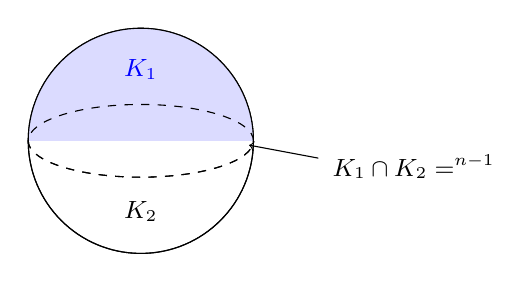
\begin{tikzpicture}[scale=1.1]
	\draw[thin] (0,0) circle (1.3);
	\draw[thin, dashed] (0,0) ellipse (1.3 and 0.42);
	\fill[color=blue!14] (0,0) ++(0:1.3) arc (0:180:1.3) -- cycle;
	\draw[thin] (0,0) circle (1.3);
	\draw[thin, dashed] (0,0) ellipse (1.3 and 0.42);
	\node[color=blue] at (0,0.82) {\small $K_1$};
	\node at (0,-0.82) {\small $K_2$};
	\node at (3.15,-0.3) {\small $K_1\cap K_2 = \sS^{n-1}$};
	\draw[thin, ->] (2.05,-0.2) -- (1.25,-0.05);
\end{tikzpicture}
\end{center}

\section{The Topological Invariance of Homology}

So far homology is an invariant of a \emph{simplicial complex}, not of a space: we have
computed $H_\bullet(K)$, and we noticed in Example \ref{ex:homology-circle} that the
answer for the $n$-gon did not depend on $n$, but we have not shown that this is a
general phenomenon. In this section we show that $H_\bullet(K)$ depends only on the
homotopy type of $|K|$, and that continuous maps induce homomorphisms. The tool is
simplicial approximation.

\subsection{Approximations are Chain Homotopic}

\begin{lemma} \label{lem:two-approximations}
	Let $f_0, f_1: K \to L$ be simplicial approximations to the same continuous map $F: |K|\to|L|$. Then for every $\sigma \in K$ there is a simplex $\tau \in L$ containing $f_0(v)$ and $f_1(v)$ for every vertex $v$ of $\sigma$.
\end{lemma}
\begin{proof}
	Pick $x \in \sigma^\circ$ and let $\tau \in L$ be the unique simplex with $F(x)\in\tau^\circ$. For each vertex $v$ of $\sigma$ we have $x \in \St_K(v)$, so $F(x) \in \St_L(f_i(v))$ for $i = 0,1$; and by Lemma \ref{lem:star}(i) this says $f_i(v) \in V(\tau)$.
\end{proof}

\begin{theorem} \label{thm:approx-chain-homotopic}
	Let $f_0, f_1: K \to L$ be simplicial approximations to the same $F: |K|\to|L|$. Then $f_{0\sharp}\simeq f_{1\sharp}$, and hence $f_{0*} = f_{1*}: H_\bullet(K)\to H_\bullet(L)$.
\end{theorem}
\begin{proof}
	Define the \vocab{prism operator} $h: C_k(K)\to C_{k+1}(L)$ on basis elements by
	$$
	h(e_{i_0\cdots i_k}) = \sum_{j=0}^k (-1)^j\, e_{\hat f_0(i_0)\cdots \hat f_0(i_j)\hat f_1(i_j)\cdots \hat f_1(i_k)} .
	$$
	Each term is a legitimate element of $C_{k+1}(L)$: by Lemma \ref{lem:two-approximations} all the indices appearing lie in the vertex set of a single simplex $\tau\in L$, so the corresponding face of $\tau$ lies in $L$ (or the term is zero, if an index repeats).

	It is now a direct computation with the formula of Proposition \ref{prop:d-general} that
	$$
	dh + hd = f_{1\sharp}-f_{0\sharp}.
	$$
	Indeed, expanding $d h(e_I)$, the terms in which one deletes an index other than the two `middle' ones $\hat f_0(i_j), \hat f_1(i_j)$ are precisely the terms of $-h(d e_I)$, with matching signs. The terms where one of the middle indices is deleted telescope: deleting $\hat f_1(i_j)$ from the $j$th summand cancels against deleting $\hat f_0(i_{j+1})$ from the $(j+1)$st, leaving only the two extreme terms, namely $e_{\hat f_1(i_0)\cdots \hat f_1(i_k)} = f_{1\sharp}(e_I)$ from $j=0$ and $-e_{\hat f_0(i_0)\cdots\hat f_0(i_k)} = -f_{0\sharp}(e_I)$ from $j = k$.

	So $h$ is a chain homotopy, and Lemma \ref{lem:chain-homotopy} gives $f_{0*} = f_{1*}$.
\end{proof}

The picture is the same prism as before: $h(\sigma)$ is the simplicial subdivision of
$\sigma\times I$, with $f_0(\sigma)$ at the bottom and $f_1(\sigma)$ at the top.

\subsection{Induced Maps}

To define $F_*$ for a continuous $F$, we approximate; but the approximation lives on a
subdivision of $K$, so we need to know that subdividing does not change homology.

\begin{theorem} \label{thm:nu}
	Let $K$ be a simplicial complex. Any simplicial approximation $g: \bary(K)\to K$ to the identity map on $|K| = |\bary(K)|$ induces an isomorphism
	$$
	\nu_K = g_*: H_\bullet(\bary(K)) \longrightarrow H_\bullet(K),
	$$
	and $\nu_K$ does not depend on the choice of $g$.
\end{theorem}
\begin{proof}[Proof sketch]
	Independence of the choice is Theorem \ref{thm:approx-chain-homotopic}, since any two such $g$ are simplicial approximations to the same map $\id$. (Note that such a $g$ exists: for each vertex $w$ of $\bary(K)$ we have $w \in \sigma^\circ$ for a unique $\sigma\in K$, and we may take $\hat g(w)$ to be any vertex of $\sigma$.)

	For the isomorphism, one induces on the skeleta of $K$. For $K$ a single simplex both $H_\bullet(\bary(K))$ and $H_\bullet(K)$ are the homology of a point, by Corollary \ref{cor:cone-homology}, and $g_*$ is easily checked to be an isomorphism there. For the inductive step one writes $K$ as the union of its $(n-1)$-skeleton and its $n$-simplices, compares the two Mayer--Vietoris sequences using the fact that $g$ is compatible with the decomposition, and applies the five lemma.
\end{proof}

Writing $\nu_{K,r}: H_\bullet(\bary^r(K))\to H_\bullet(K)$ for the composite
$\nu_K \circ \nu_{\bary(K)}\circ\cdots$, we can now make the key definition.

\begin{definition} \label{def:induced-homology}
	Let $F: |K|\to|L|$ be continuous. By the simplicial approximation theorem there is a simplicial $f: \bary^r(K)\to L$ with $|f|\simeq F$. Define
	$$
	F_* = f_* \circ \nu_{K,r}^{-1}: H_\bullet(K) \longrightarrow H_\bullet(L).
	$$
\end{definition}

\begin{theorem} \label{thm:functorial-homology}
	$F_*$ is well-defined, independent of the choice of $r$ and $f$. Moreover $(\id)_* = \id$ and $(F\circ G)_* = F_*\circ G_*$.
\end{theorem}
\begin{proof}[Proof sketch]
	If $f: \bary^r(K)\to L$ and $f': \bary^{r'}(K)\to L$ are two simplicial approximations to $F$, with $r \leq r'$ say, choose a simplicial approximation $g: \bary^{r'}(K)\to\bary^r(K)$ to the identity. Then $f\circ g$ and $f'$ are both simplicial approximations to $F$, so $f_*g_* = f'_*$ by Theorem \ref{thm:approx-chain-homotopic}; and $g_* = \nu_{\bary^r(K), r'-r}$, so $f'_*\nu_{K,r'}^{-1} = f_*\nu_{K,r}^{-1}$.

	Functoriality follows similarly: if $f$ approximates $F$ and $g$ approximates $G$ (after enough subdivision that the composite makes sense), then $f\circ g$ approximates $F \circ G$.
\end{proof}

\begin{theorem}[Homotopy Invariance] \label{thm:homotopy-invariance}
	If $F_0, F_1: |K|\to|L|$ are continuous with $F_0 \simeq F_1$, then $F_{0*} = F_{1*}$.
\end{theorem}
\begin{proof}[Proof sketch]
	Let $H: |K|\times I \to |L|$ be a homotopy. Triangulate $|K|\times I$, which is the polyhedron of a simplicial complex $M$ containing two copies $K^0, K^1$ of $K$ at the ends. Applying simplicial approximation to $H$ gives a simplicial map $\bary^r(M)\to L$ restricting on the two ends to approximations of $F_0$ and $F_1$; the inclusions of the ends are homotopy equivalences onto $|M|$ inducing the same map on homology, by the argument of Theorem \ref{thm:approx-chain-homotopic} applied to the prism. Hence $F_{0*} = F_{1*}$.
\end{proof}

\begin{corollary} \label{cor:homotopy-invariance}
	If $|K| \simeq |L|$ then $H_\bullet(K)\cong H_\bullet(L)$.
\end{corollary}
\begin{proof}
	Let $F: |K|\to|L|$ and $G: |L|\to|K|$ with $F\circ G \simeq \id$ and $G \circ F \simeq \id$. Then by Theorems \ref{thm:functorial-homology} and \ref{thm:homotopy-invariance}, $F_*G_* = \id$ and $G_*F_* = \id$, so $F_*$ is an isomorphism.
\end{proof}

\begin{definition}
	A space $X$ is \vocab{triangulable} if $X \cong |K|$ for some simplicial complex $K$. In that case we define $H_\bullet(X) = H_\bullet(K)$, which by Corollary \ref{cor:homotopy-invariance} is well-defined.
\end{definition}

Not every space is triangulable, or even homotopy equivalent to a triangulable space --- the
infinite wedge $\bigvee_{i=1}^\infty S^1$ is an example --- but every compact manifold and
every CW complex we shall meet is.

\subsection{First Consequences}

\begin{proposition} \label{prop:h0}
	If $|K|$ is path connected then $H_0(K)\cong\Z$. In general $H_0(K)\cong\Z^k$ where $k$ is the number of path components of $|K|$.
\end{proposition}
\begin{proof}
	$C_0(K)$ is free on the vertices $e_i$, and every $e_i$ is a cycle. For vertices $e_i, e_j$, let $F_i: \Delta^0 \to |K|$ be the map hitting $e_i$; then $F_{i*}[e_0] = [e_i]$. If $|K|$ is path connected then $F_i \simeq F_j$, so $[e_i] = [e_j]$ by homotopy invariance. Hence $H_0(K)$ is generated by the single class $[e_0]$. It is non-trivial: the homomorphism $C_0(K)\to\Z$ sending each $e_i \mapsto 1$ kills $\operatorname{im}d_1$ (as $d(e_{ij}) = e_j - e_i$), so it descends to a surjection $H_0(K)\to\Z$. Hence $H_0(K)\cong\Z$.

	In general $|K|$ is the disjoint union of its path components, each of which is the polyhedron of a subcomplex, and Example \ref{ex:disjoint} gives the direct sum decomposition.
\end{proof}

\begin{theorem} \label{thm:sphere-homology-space}
	For $n \geq 1$,
	$$
	H_k(S^n) = \begin{cases}\Z & k = 0, n\\ 0 & \text{otherwise},\end{cases}
	$$
	and $H_k(D^n) = \Z$ for $k = 0$, zero otherwise. Consequently $S^n \simeq S^m$ implies $n = m$.
\end{theorem}
\begin{proof}
	We have $S^n \cong |\sS^n|$ and $D^n \cong |\bDelta^n|$, so this is Theorem \ref{thm:homology-spheres} and Corollary \ref{cor:cone-homology}. If $S^n \simeq S^m$ with $n \neq m$, comparing $H_n$ gives $\Z \cong 0$ (taking $n \geq 1$; the case $n = 0$ is clear as $S^0$ is disconnected).
\end{proof}

\begin{corollary}[Invariance of Dimension]
	If $\R^n \cong \R^m$ then $n = m$.
\end{corollary}
\begin{proof}
	Take $n, m \geq 1$. A homeomorphism $f: \R^n \to \R^m$ restricts to a homeomorphism $\R^n\setminus\{0\}\to\R^m\setminus\{f(0)\}$. By Example \ref{ex:sdr-sphere} these are homotopy equivalent to $S^{n-1}$ and $S^{m-1}$ respectively, so $S^{n-1}\simeq S^{m-1}$ and hence $n = m$ by Theorem \ref{thm:sphere-homology-space}.
\end{proof}

\begin{corollary} \label{cor:no-retraction}
	For $n \geq 1$ there is no retraction $r: D^n \to S^{n-1}$.
\end{corollary}
\begin{proof}
	Let $j: S^{n-1}\hookrightarrow D^n$ be the inclusion. If $r$ were a retraction then $r\circ j = \id$, so $r_*j_* = \id$ on $H_{n-1}(S^{n-1})$. For $n \geq 2$ this is $\Z$, while $H_{n-1}(D^n) = 0$, so the identity on $\Z$ factors through $0$, which is absurd. For $n = 1$ use $H_0$: $H_0(S^0) = \Z^2$ and $H_0(D^1) = \Z$, and $\Z^2 \to \Z \to \Z^2$ cannot compose to the identity.
\end{proof}

\begin{theorem}[Brouwer Fixed Point Theorem] \label{thm:brouwer}
	Every continuous $F: D^n \to D^n$ has a fixed point.
\end{theorem}
\begin{proof}
	Suppose not, so $F(x)\neq x$ for all $x$. Define $G: D^n \to S^{n-1}$ by letting $G(x)$ be the point where the ray from $F(x)$ through $x$ meets $S^{n-1}$; we must check this is continuous.

	For $p \in D^n$ and $v\in S^{n-1}$, the ray $\{p+tv \mid t \geq 0\}$ meets $S^{n-1}$ where $\norm{p+tv}^2 = 1$, that is
	$$
	t^2 + 2t\langle p,v\rangle + \norm{p}^2 - 1 = 0, \qquad t = -\langle p,v\rangle \pm \sqrt{\langle p,v\rangle^2+1-\norm{p}^2},
	$$
	and the discriminant is non-negative since $\norm{p}\leq 1$. Taking the larger root,
	$$
	\tau(p,v) = -\langle p,v\rangle + \sqrt{\langle p,v\rangle^2+1-\norm{p}^2}
	$$
	is continuous in $(p,v)$, and so is $P(p,v) = p + \tau(p,v)v$. Hence
	$$
	G(x) = P\left(F(x), \frac{x-F(x)}{\norm{x-F(x)}}\right)
	$$
	is continuous, using $x \neq F(x)$. If $x \in S^{n-1}$ then $x$ itself lies on the ray and on the sphere with $t > 0$, so $G(x) = x$. Thus $G$ is a retraction $D^n \to S^{n-1}$, contradicting Corollary \ref{cor:no-retraction}.
\end{proof}

\section{Homology Calculations and Applications}

We now have a working invariant. In this final section we put it to work: we define the
degree of a map of spheres, compute the homology of all the closed surfaces, and
establish the Euler characteristic and the Lefschetz fixed point theorem.

\subsection{Degree}

Since $H_n(S^n)\cong\Z$ for $n \geq 1$, any map $f: S^n \to S^n$ induces a homomorphism
$\Z\to\Z$, which is multiplication by an integer.

\begin{definition}[Degree]
	For $n \geq 1$ and $f: S^n \to S^n$, the \vocab{degree} $\deg f \in \Z$ is defined by
	$$
	f_*(x) = (\deg f)\, x \quad \text{for all } x \in H_n(S^n)\cong\Z.
	$$
\end{definition}

Note that this is independent of the choice of generator, since $-1$ times a generator
gives the same multiplier.

\begin{proposition} \label{prop:degree-props}
	For maps $f, g: S^n \to S^n$:
	\begin{enumerate}
		\item $\deg\id = 1$ and $\deg(g\circ f) = \deg g \cdot \deg f$;
		\item if $f \simeq g$ then $\deg f = \deg g$;
		\item if $f$ is constant then $\deg f = 0$;
		\item if $f$ is a homotopy equivalence then $\deg f = \pm 1$.
	\end{enumerate}
\end{proposition}
\begin{proof}
	(i) is functoriality (Theorem \ref{thm:functorial-homology}) and (ii) is homotopy invariance (Theorem \ref{thm:homotopy-invariance}). For (iii), a constant map factors through a point, and $H_n(*) = 0$ for $n \geq 1$. For (iv), if $g$ is a homotopy inverse then $\deg g \deg f = \deg\id = 1$ in $\Z$.
\end{proof}

\begin{corollary}
	$\id_{S^n}$ is not null-homotopic, so $S^n$ is not contractible.
\end{corollary}
\begin{proof}
	$\deg \id = 1 \neq 0 = \deg(\text{constant})$.
\end{proof}

Together with Theorem \ref{thm:sk-to-sn} this completes the story we began in Section
\ref{sec:simplicial}: for $k < n$ every map $S^k \to S^n$ is null-homotopic, whereas
$\id_{S^n}$ is not, so $S^k \not\simeq S^n$.

For $n = 1$ this notion of degree agrees with the one we defined via $\pi_1$ in
Section 2, since both are computed by the winding number of the image loop --- for
instance, $z \mapsto z^m$ has degree $m$ in both senses.

\begin{example}
	Let $r: S^n \to S^n$ be the reflection $(x_0,\dots,x_n)\mapsto(-x_0,x_1,\dots,x_n)$. Then $\deg r = -1$. To see this, triangulate $S^n$ as $|\sS^n|$ so that $r$ is simplicial and swaps two vertices $e_0 \leftrightarrow e_1$, fixing the rest; then $r_\sharp$ acts on the top cycle by transposing two indices, hence by $-1$. Consequently the antipodal map $a = (-1)^{\text{all coordinates}}$, being a composite of $n+1$ reflections, has $\deg a = (-1)^{n+1}$.
\end{example}

\subsection{The Homology of Surfaces}

We first record a splitting lemma, which lets us read off answers from short exact
sequences.

\begin{proposition} \label{prop:splitting}
	If $0 \to A \to B \to \Z^r \to 0$ is exact, then $B \cong A \oplus \Z^r$.
\end{proposition}
\begin{proof}
	Choose $b_i \in B$ mapping to the standard basis vectors of $\Z^r$; this defines a homomorphism $s: \Z^r \to B$ splitting the surjection, since $\Z^r$ is free. Then $b \mapsto (b - s(g(b)), g(b))$ is an isomorphism $B \to A \oplus \Z^r$.
\end{proof}

\begin{example}[The Torus] \label{ex:torus-homology}
	Triangulate $T^2$ as $|K|$ and write $K = K_1 \cup K_2$, where $|K_1|$ and $|K_2|$ are the two cylinders obtained by cutting the torus along two parallel circles. Then $|K_i|\simeq S^1$ and $|K_1\cap K_2| \cong S^1 \sqcup S^1$.

	Both inclusions $S^1 \hookrightarrow |K_i|$ of the two boundary circles are homotopy equivalences, and they are homotopic to each other. So on $H_1$, writing $c_1, c_2$ for the classes of the two circles of the intersection, the map $\alpha_1 = i_*$ has matrix
	$$
	\alpha_1 = \begin{pmatrix}1&1\\1&1\end{pmatrix}: \Z^2 \to \Z^2 ,
	$$
	and the same is true of $\alpha_0$ on $H_0$. Hence $\ker\alpha_k \cong \Z$ and $\coker\alpha_k\cong\Z$ for $k = 0,1$.

	Since $H_2(K_i) = H_2(S^1) = 0$, the Mayer--Vietoris sequence
	\begin{align*}
		0 \to H_2(K) &\xrightarrow{\ \partial\ } H_1(K_1\cap K_2) \xrightarrow{\ \alpha_1\ } H_1(K_1)\oplus H_1(K_2) \to H_1(K)\\
		&\xrightarrow{\ \partial\ } H_0(K_1\cap K_2) \xrightarrow{\ \alpha_0\ } H_0(K_1)\oplus H_0(K_2) \to H_0(K) \to 0
	\end{align*}
	breaks into short exact sequences
	\begin{align*}
		&0 \to H_2(K)\to\ker\alpha_1\to 0, \qquad 0\to\coker\alpha_0\to H_0(K)\to0,\\
		&0 \to \coker\alpha_1 \to H_1(K)\to\ker\alpha_0\to0.
	\end{align*}
	Therefore $H_2(T^2)\cong\Z$, and $H_1(T^2)\cong\Z\oplus\Z$ by Proposition \ref{prop:splitting}, and $H_0(T^2)\cong\Z$. In summary
	$$
	H_k(T^2) = \begin{cases}\Z & k = 0,2\\ \Z^2 & k=1\\ 0&\text{otherwise.}\end{cases}
	$$
\end{example}

\begin{center}
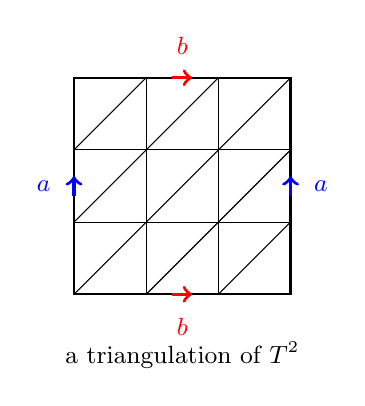
\begin{tikzpicture}[scale=1.25]
	\draw[thick] (0,0) rectangle (2.2,2.2);
	\draw[thin] (0,0) -- (2.2,2.2);
	\draw[thin] (0,0.7333) -- (1.4667,2.2);
	\draw[thin] (0,1.4667) -- (0.7333,2.2);
	\draw[thin] (0.7333,0) -- (2.2,1.4667);
	\draw[thin] (1.4667,0) -- (2.2,0.7333);
	\foreach \x in {0.7333,1.4667} { \draw[thin] (\x,0) -- (\x,2.2); }
	\foreach \y in {0.7333,1.4667} { \draw[thin] (0,\y) -- (2.2,\y); }
	\draw[->, very thick, color=blue] (0,1.0) -- (0,1.2);
	\draw[->, very thick, color=blue] (2.2,1.0) -- (2.2,1.2);
	\draw[->, very thick, color=red] (1.0,0) -- (1.2,0);
	\draw[->, very thick, color=red] (1.0,2.2) -- (1.2,2.2);
	\node[color=blue, left] at (-0.14,1.1) {\small $a$};
	\node[color=blue, right] at (2.34,1.1) {\small $a$};
	\node[color=red, below] at (1.1,-0.14) {\small $b$};
	\node[color=red, above] at (1.1,2.34) {\small $b$};
	\node at (1.1,-0.62) {\small a triangulation of $T^2$};
\end{tikzpicture}
\end{center}

For higher genus it is cleanest to build the surface out of a wedge of circles and a
single disc, exactly as in Example \ref{ex:genus-g}. Write $\Sigma_{g,1}$ for the surface
$\Sigma_g$ with an open disc removed.

\begin{lemma} \label{lem:punctured-surface}
	$\Sigma_{g,1} \simeq \bigvee_{i=1}^{2g}S^1$, and hence
	$$
	H_k(\Sigma_{g,1}) = \begin{cases}\Z & k=0\\ \Z^{2g} & k=1\\ 0 & \text{otherwise.}\end{cases}
	$$
\end{lemma}
\begin{proof}
	Realise $\Sigma_g$ as a $4g$-gon with its boundary identified, and remove an open disc from the interior. What is left deformation retracts radially onto the boundary of the polygon, which after the identifications is $\bigvee_{i=1}^{2g}S^1$. The homology of a wedge of $m$ circles is $H_0 = \Z$, $H_1 = \Z^m$ and $0$ above --- by induction on $m$ using Mayer--Vietoris with $K_1$ the first circle and $K_2$ the rest (thickened slightly so as to intersect in a contractible set).
\end{proof}

\begin{theorem} \label{thm:genus-homology}
	For the closed orientable surface of genus $g \geq 0$,
	$$
	H_k(\Sigma_g) = \begin{cases}\Z & k = 0, 2\\ \Z^{2g} & k = 1\\ 0 & \text{otherwise.}\end{cases}
	$$
\end{theorem}
\begin{proof}
	Write $\Sigma_g = K_1 \cup K_2$ with $|K_1| = \Sigma_{g,1}$ and $|K_2| = D^2$ the disc we removed, so $|K_1\cap K_2| \cong S^1$. Mayer--Vietoris gives
	\begin{align*}
		0 \to H_2(\Sigma_g) &\xrightarrow{\ \partial\ } H_1(S^1) \xrightarrow{\ \iota_*\ } H_1(\Sigma_{g,1}) \to H_1(\Sigma_g)\\
		&\xrightarrow{\ \partial\ } H_0(S^1) \xrightarrow{\ \alpha_0\ } H_0(K_1)\oplus H_0(K_2),
	\end{align*}
	using $H_2(K_i) = 0$ from Lemma \ref{lem:punctured-surface} and Corollary \ref{cor:cone-homology}.

	The key point is that $\iota_*: \Z\to\Z^{2g}$ is the zero map. Under the identification of Lemma \ref{lem:punctured-surface}, the boundary circle is the loop
	$$
	a_1b_1a_1^{-1}b_1^{-1}\cdots a_gb_ga_g^{-1}b_g^{-1},
	$$
	whose class in $H_1(\bigvee S^1) = \Z^{2g}$ is obtained by adding up the signed number of times it traverses each circle. Each generator occurs once forwards and once backwards, so the total is $0$.

	Hence $\partial: H_2(\Sigma_g)\to\Z$ is an isomorphism onto $\ker\iota_* = \Z$, giving $H_2(\Sigma_g)\cong\Z$. Also $\Z^{2g} = \coker\iota_* \hookrightarrow H_1(\Sigma_g)$, and $\alpha_0: \Z\to\Z^2$ is injective (both components send a point to a point), so $\partial = 0$ on $H_1$ and the map $\Z^{2g}\to H_1(\Sigma_g)$ is onto. So $H_1(\Sigma_g)\cong\Z^{2g}$. Finally $H_0(\Sigma_g)\cong\Z$ by connectedness. For $g = 0$ this reduces to $H_\bullet(S^2)$, as it should.
\end{proof}

The same argument handles the non-orientable surfaces. Let $N_r$ be the closed surface
obtained from a $2r$-gon by identifying the edges according to the word
$a_1^2a_2^2\cdots a_r^2$; equivalently, $N_r$ is the connected sum of $r$ copies of
$\RP^2$. So $N_1 = \RP^2$ and $N_2 = K$, the Klein bottle, and $N_{r,1}$, the surface with
an open disc removed, is homotopy equivalent to $\bigvee_{i=1}^r S^1$. For $r = 1$ the
punctured surface $N_{1,1}$ is the M\"obius band, and its boundary circle wraps
\emph{twice} around the core.

\begin{center}
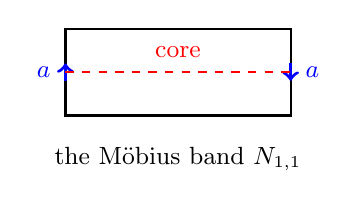
\begin{tikzpicture}[scale=1.1]
	\draw[thick] (0,0) rectangle (2.6,1.0);
	\draw[->, very thick, color=blue] (0,0.4) -- (0,0.6);
	\draw[->, very thick, color=blue] (2.6,0.6) -- (2.6,0.4);
	\node[color=blue, left] at (-0.06,0.5) {\small $a$};
	\node[color=blue, right] at (2.66,0.5) {\small $a$};
	\draw[thick, dashed, color=red] (0,0.5) -- (2.6,0.5);
	\node[color=red, above] at (1.3,0.55) {\small core};
	\node at (1.3,-0.5) {\small the M\"obius band $N_{1,1}$};
\end{tikzpicture}
\end{center}

\begin{theorem} \label{thm:nonorientable-homology}
	For $r \geq 1$,
	$$
	H_k(N_r) = \begin{cases}\Z & k = 0\\ \Z^{r-1}\oplus \Z/2\Z & k = 1\\ 0 & \text{otherwise.}\end{cases}
	$$
	In particular $H_2(N_r) = 0$ and $H_1(\RP^2) = \Z/2\Z$.
\end{theorem}
\begin{proof}
	As before, $N_r = N_{r,1}\cup D^2$ with $N_{r,1}\simeq\bigvee_{i=1}^rS^1$ and intersection $S^1$. This time the attaching loop is $a_1^2\cdots a_r^2$, whose class in $H_1 = \Z^r$ is $(2,2,\dots,2)$. So $\iota_*: \Z\to\Z^r$ is injective, whence $H_2(N_r) = \ker\iota_* = 0$, and
	$$
	H_1(N_r) \cong \coker\iota_* = \Z^r/\genby{(2,\dots,2)}.
	$$
	Changing basis to $u_1 = e_1+\dots+e_r$, $u_2 = e_2,\dots,u_r = e_r$, this is $\Z^r/\genby{2u_1}\cong \Z/2\Z\oplus\Z^{r-1}$, as claimed. (As in the orientable case, $\alpha_0$ is injective so the sequence terminates correctly.)
\end{proof}

Notice that homology detects non-orientability through torsion, and through the vanishing
of $H_2$: a closed orientable surface has a fundamental class in $H_2$, and a
non-orientable one does not. In particular the $\Sigma_g$ and $N_r$ are pairwise
non-homotopy-equivalent, which together with the classification of surfaces says that
homology is a complete invariant for closed surfaces.

\subsection{The Euler Characteristic}

\begin{definition}[Euler Characteristic]
	Let $K$ be a simplicial complex. Its \vocab{Euler characteristic} is
	$$
	\chi(K) = \sum_k(-1)^k \operatorname{rank}C_k(K),
	$$
	the alternating sum of the numbers of simplices in each dimension.
\end{definition}

For a two-dimensional complex this is `vertices $-$ edges $+$ faces', the classical Euler
formula. It is not at all obvious from the definition that this depends only on $|K|$,
but homology makes it so.

\begin{theorem} \label{thm:euler}
	$\displaystyle \chi(K) = \sum_k(-1)^k\operatorname{rank}H_k(K)$. In particular $\chi(K)$ depends only on the homotopy type of $|K|$.
\end{theorem}
\begin{proof}
	Write $Z_k = \ker d_k$ and $B_k = \operatorname{im}d_{k+1}$, both subgroups of the free abelian group $C_k$, hence free. Rank-nullity applied to $d_k: C_k \to C_{k-1}$, whose image is $B_{k-1}$, gives
	$$
	\operatorname{rank}C_k = \operatorname{rank}Z_k + \operatorname{rank}B_{k-1},
	$$
	and $H_k = Z_k/B_k$ gives $\operatorname{rank}Z_k = \operatorname{rank}H_k + \operatorname{rank}B_k$. Hence
	$$
	\sum_k(-1)^k\operatorname{rank}C_k = \sum_k(-1)^k(\operatorname{rank}H_k + \operatorname{rank}B_k + \operatorname{rank}B_{k-1}),
	$$
	and the $B$ terms cancel in pairs, leaving $\sum_k(-1)^k\operatorname{rank}H_k$.
\end{proof}

\begin{example}
	From Theorems \ref{thm:genus-homology} and \ref{thm:nonorientable-homology},
	$$
	\chi(\Sigma_g) = 1 - 2g + 1 = 2-2g, \qquad \chi(N_r) = 1 - (r-1) + 0 = 2 - r,
	$$
	using that $\Z/2\Z$ has rank $0$. So $\chi(S^2) = 2$, $\chi(T^2) = 0$, $\chi(\RP^2) = 1$ and $\chi(K) = 0$ for the Klein bottle. Also $\chi(S^n) = 1+(-1)^n$.
\end{example}

\subsection{The Lefschetz Fixed Point Theorem}

Brouwer's theorem said that a self-map of a disc has a fixed point. There is a beautiful
generalisation, which computes an obstruction to being fixed-point-free out of the
induced maps on homology. For this it is convenient to work with rational coefficients:
replacing each $C_k(K) \cong \Z^{n_k}$ by $\Q^{n_k}$ with the same boundary matrices gives
a chain complex of $\Q$-vector spaces, and all the theory goes through verbatim, with
$H_k(K;\Q)$ a vector space of dimension $\operatorname{rank}H_k(K)$.

\begin{definition}[Lefschetz Number]
	Let $f: C \to C$ be a chain map of a finitely generated chain complex of $\Q$-vector spaces. Its \vocab{Lefschetz number} is
	$$
	L(f) = \sum_k (-1)^k \tr(f_k: C_k \to C_k),
	$$
	and likewise $L(f_*) = \sum_k(-1)^k\tr(f_{k*}: H_k(C)\to H_k(C))$.
\end{definition}

\begin{proposition} \label{prop:lefschetz-trace}
	$L(f) = L(f_*)$.
\end{proposition}
\begin{proof}
	Write $U_k = \operatorname{im}d_{k+1}\subseteq \ker d_k\subseteq C_k$, and choose complements so that $\ker d_k = U_k\oplus V_k$ and $C_k = U_k\oplus V_k\oplus U_k'$. Then $d$ maps $U_k'$ isomorphically onto $U_{k-1}$ and kills $U_k\oplus V_k$, so in block form
	$$
	d = \begin{pmatrix}0&0&I\\0&0&0\\0&0&0\end{pmatrix}.
	$$
	Since $f$ is a chain map it preserves $\ker d$ and $\operatorname{im}d$, so
	$$
	f_k = \begin{pmatrix}A_k & X_k & *\\ 0 & B_k & *\\ 0&0&A_k'\end{pmatrix},
	$$
	and comparing $df = fd$ in the top-right block gives $A_{k-1} = A_k'$. Now $H_k(C) = (U_k\oplus V_k)/U_k \cong V_k$, on which $f_{k*}$ acts by $B_k$. Hence
	$$
	L(f) = \sum_k(-1)^k(\tr A_k + \tr B_k + \tr A_{k-1}) = \sum_k(-1)^k\tr B_k = L(f_*),
	$$
	because the $A$ terms cancel in consecutive pairs.
\end{proof}

\begin{corollary}
	$\chi(K) = L(\id) = L(\id_{H_\bullet})$, recovering Theorem \ref{thm:euler}.
\end{corollary}

\begin{definition}
	For a continuous $F: |K|\to|K|$, its \vocab{Lefschetz number} is $L(F) = L(F_*)$, where $F_*: H_\bullet(K;\Q)\to H_\bullet(K;\Q)$.
\end{definition}

\begin{theorem}[Lefschetz Fixed Point Theorem] \label{thm:lefschetz}
	Let $K$ be a simplicial complex and $F: |K|\to|K|$ continuous. If $L(F)\neq 0$ then $F$ has a fixed point.
\end{theorem}
\begin{proof}[Proof sketch]
	Suppose $F$ has no fixed point. As $|K|$ is compact and $x \mapsto \norm{F(x)-x}$ is continuous and positive, there is $\varepsilon>0$ with $\norm{F(x)-x}\geq\varepsilon$ for all $x$.

	Subdivide until $\mu(\bary^r K) < \varepsilon/3$, and take a simplicial approximation $f: \bary^{r+s}(K)\to\bary^r(K)$ to $F$ for suitable $s$. Then for each simplex $\sigma$ of $\bary^{r+s}(K)$, the image $f(\sigma)$ is at distance at least $\varepsilon/3$ from $\sigma$, so $f(\sigma)\neq\sigma$; that is, no basis element of the chain complex is sent to a multiple of itself. Hence every diagonal entry of every matrix $f_k$ vanishes, so $L(f) = 0$, and by Proposition \ref{prop:lefschetz-trace} and the identification of $f_*$ with $F_*$ we get $L(F) = 0$.
\end{proof}

\begin{example}
	If $|K|$ is contractible then $H_0 = \Q$ and $H_k = 0$ for $k > 0$, and $F_{0*} = \id$ on $H_0$ since $|K|$ is connected. So $L(F) = 1 \neq 0$ for every $F$, and every self-map of a contractible polyhedron has a fixed point. Taking $|K| = D^n$ recovers the Brouwer fixed point theorem.
\end{example}

\begin{example}
	Let $F: S^n \to S^n$. Then $L(F) = 1 + (-1)^n\deg F$. So if $\deg F \neq (-1)^{n+1}$ then $F$ has a fixed point. In particular any map $S^n \to S^n$ without a fixed point has the degree of the antipodal map, and any map of $S^{2n}$ of degree $1$ --- for instance any orientation-preserving homeomorphism --- has a fixed point.
\end{example}

\begin{example}
	Let $F: \Sigma_g \to \Sigma_g$ with $g \geq 2$, and suppose $F$ acts as the identity on $H_1$. Then
	$$
	L(F) = 1 - 2g + \tr(F_{2*}),
	$$
	where $F_{2*}$ is multiplication by the degree $d$ of $F$. So $L(F) = 1-2g+d$, and $F$ has a fixed point unless $d$ happens to equal $2g-1$. For example, any such $F$ of degree $1$ has a fixed point once $g \geq 2$.
\end{example}

We finish with a remark on where all this goes. Simplicial homology is concrete, and that
is its virtue for a first course, but the price is the enormous labour of the invariance
theorems: we had to subdivide, approximate, and compare, simply to know that
$H_\bullet(K)$ depends only on $|K|$. \emph{Singular} homology, in which one takes the
free abelian group on \emph{all} continuous maps $\Delta^n \to X$, is manifestly a
topological invariant and is defined for every space; the price there is that the chain
groups are enormous and nothing can be computed directly. The two theories agree on
triangulable spaces, and the modern approach is to use singular homology for the theory
and simplicial (or cellular) homology for the computations --- which is, in effect, what
we have been doing all along.

